\documentclass[DIV=14,parskip=full,pointednumbers]{scrartcl}
%\setcounter{equation}{0}
\usepackage[utf8]{inputenc}
\setkomafont{sectioning}{\rmfamily\bfseries}

\usepackage{amsmath,amsfonts,amssymb,mathtools}
\usepackage{amsthm}
%\usepackage{halloweenmath}
\usepackage{xstring,verbatim}
\usepackage{bm}

\usepackage{stmaryrd}

\usepackage{old-arrows}
\usepackage{pgf,tikz}
\usetikzlibrary{positioning,arrows,calc}
\usepackage[shortlabels]{enumitem}
\setlist[description]{font={\bfseries\rmfamily}}

\usepackage[english]{babel}
\usetikzlibrary{calc}
\usepackage{subcaption}

\usepackage[colorlinks=true,linkcolor=blue]{hyperref}

\renewcommand{\phi}{\varphi}
\title{Algebraic Geometry 0.5 (a.k.a. Algebra I)}
\author{Nicholas Schwab \&\ Ferdinand Wagner}
\date{Sommersemester 2017}

\newenvironment{alphanumerate}{\begin{enumerate}[label={$(\alph*)$},ref=\curthm]}{\end{enumerate}}       
%\newenvironment{rmnumerate}{\begin{enumerate}[label={\upshape(\roman*)},ref=\curthm]}{\end{enumerate}}   
\renewenvironment{itemize}{\begin{enumerate}[label={$\bullet$},ref=\curthm]}{\end{enumerate}}
\newenvironment{diagram}{\begin{center}\begin{tikzpicture}}{\end{tikzpicture}\end{center}}  

\def\newnewtheorem#1#2[#3]{\newtheorem{#1}{#2}[#3]\expandafter\def\csname thmcaption#1\endcsname{#2}}%erstellt zusätzlich ein Makro, das den Umgebungsnamen enthält                               

\newtheoremstyle{cthm}
{12pt}
{0pt}
{\itshape}
{}
{\bfseries}
{.}
{ }
{\thmname{#1}\thmnumber{ \IfBeginWith{#2}{\thesubsection.}{\StrBehind{#2}{\thesubsection.}}{#2}}\thmnote{ \textmd{(#3)}}\xdef\curthm{#2}}

\newtheoremstyle{cvarthm}
{12pt}
{0pt}
{\itshape}
{}
{\bfseries}
{.}
{ }
{\edef\curthmnumber{\csname the\thmenv\endcsname}\thmname{\csname thmcaption\thmenv\endcsname}\thmnumber{ \IfBeginWith{\curthmnumber}{\thesubsection.}{\StrBehind{\curthmnumber a}{\thesubsection.}}{\curthmnumber a}}\thmnote{ \textmd{(#3)}}\xdef\curthm{\curthmnumber a}}%für Varianten von Theoremen

\newtheoremstyle{cdef}
{12pt}
{0pt}
{}
{}
{\bfseries}
{.}
{ }
{\thmname{#1}\thmnumber{ \IfBeginWith{#2}{\thesubsection.}{\StrBehind{#2}{\thesubsection.}}{#2}}\thmnote{ \textmd{(#3)}}\xdef\curthm{#2}}

\theoremstyle{cthm}
\newnewtheorem{thm}{Theorem}[]
\newnewtheorem{lem}{Lemma}[subsection]
\newnewtheorem{sat}{Satz}[subsection]
\newnewtheorem{exc}{Exercise}[subsection]
\newnewtheorem{cor}{Corollary}[subsection]
\newnewtheorem{prop}{Proposition}[subsection]

\theoremstyle{cvarthm}
\newtheorem{varthmcontainer}{May differ}
\renewcommand{\thevarthmcontainer}{\csname the\thmenv\endcsname a}

\newenvironment{varthm}[1]{\gdef\thmenv{#1}\begin{varthmcontainer}}{\end{varthmcontainer}}

\renewenvironment{proof}[1][\proofname]
{\pushQED{\qed}\topsep0pt \partopsep0pt\trivlist\item[\hskip\labelsep\itshape #1.] }{\popQED\endtrivlist\addvspace{6pt plus 6pt}}

\theoremstyle{cdef}
\newtheorem{defi}{Definition}[subsection]
\newtheorem*{defi*}{Definition}
\newtheorem{example}{Example}[subsection]
\newtheorem{example*}{Example}
\newtheorem{rem}{Remark}[subsection]
\newtheorem*{rem*}{Remark}
\newtheorem{fact}{Fact}[subsection]
\newtheorem*{fact*}{Fact}


\newcommand{\lbl}[1]{
	\label{#1}
	\ifmmode
	\expandafter\xdef\csname eqsubsec#1\endcsname{\thesubsection}
	\fi
}

%\newcommand{\reff}[1]{%
%	\edef\temp{\getrefnumber{#1}}%
%	\StrBehind{\temp}{\thesubsection.}[\tempcropped]%
%	\IfBeginWith{\temp}{\thesubsection}{\hyperref[#1]{\tempcropped}}{\hyperref[#1]{\temp}}%
%}

\newcommand{\reff}[1]{%
	\edef\pretemp{\getrefnumber{#1}}%this is an
	\StrLeft{\pretemp}{1}[\dummy]%incredibly nasty
	\IfInteger{\dummy}{\def\temp{\pretemp}}{\def\temp{\detokenize\pretemp}}%kinda
	\StrBehind{\temp}{\thesubsection.}[\tempcropped]%hacky workaround
	\IfBeginWith{\temp}{\thesubsection}{\hyperref[#1]{\tempcropped}} {\hyperref[#1]{\temp}}%for some seriously weird bug
}

\newcommand{\eqreff}[1]{%
	\edef\temp{\csname eqsubsec#1\endcsname}%
	\IfBeginWith{\temp}{\thesubsection}{\hyperref[#1]{\upshape(\getrefnumber{#1})}}{\hyperref[#1]{\upshape(\temp .\getrefnumber{#1})}}%	
}

\newcommand{\Aa}{\mathcal{A}}
\newcommand{\Bb}{\mathcal{B}}
\newcommand{\Cc}{\mathcal{C}}
\newcommand{\Ll}{\mathcal{L}}
\newcommand{\Oo}{\mathcal{O}}
\newcommand{\Gg}{\mathcal{G}}

\newcommand{\IN}{\mathbb{N}}
\newcommand{\IZ}{\mathbb{Z}}
\newcommand{\IP}{\mathbb{P}}
\newcommand{\IQ}{\mathbb{Q}}
\newcommand{\IR}{\mathbb{R}}
\newcommand{\IC}{\mathbb{C}}

\renewcommand{\AA}{\mathfrak A}
\newcommand{\BB}{\mathfrak B}
\newcommand{\CC}{\mathfrak C}
\newcommand{\KK}{\mathfrak K}
\newcommand{\MM}{\mathfrak{M}}
\newcommand{\XX}{\mathfrak{X}}

\renewcommand{\aa}{\mathfrak{a}}
\newcommand{\bb}{\mathfrak{b}}
\newcommand{\kk}{\mathfrak{k}}
\newcommand{\mm}{\mathfrak{m}}
\newcommand{\nn}{\mathfrak{n}}
\newcommand{\pp}{\mathfrak{p}}
\newcommand{\qq}{\mathfrak{q}}
\newcommand{\rr}{\mathfrak{r}}

\renewcommand{\AA}{\mathfrak A}

\newcommand{\newoperator}[1]{\expandafter\def\csname #1\endcsname{\operatorname{#1}}}

\newcommand{\Hom}{\operatorname{Hom}}
\newcommand{\Ann}{\operatorname{Ann}}
\newcommand{\End}{\operatorname{End}}
\newcommand{\Aut}{\operatorname{Aut}}
\newcommand{\Gal}{\operatorname{Gal}}
\newcommand{\codim}{\operatorname{codim}}
\newcommand{\Spec}{\operatorname{Spec}}
\newoperator{sep}
\newcommand{\tr}{\operatorname{tr}}
%\newoperator{ht}
%\newoperator{char}
\newcommand{\id}{\operatorname{id}}
\newcommand{\cha}{\operatorname{char}}
\newcommand{\hoehe}{\operatorname{ht}}
\newoperator{Ob}
\newoperator{lcm}
\newcommand{\op}{^{\operatorname{op}}}
\newcommand{\mSpec}{\mm\operatorname{-Spec}}
%\newcommand{\multiline}[1]{#1}
\newcommand{\longto}{\longrightarrow}
\newcommand{\longot}{\longleftarrow}
\newcommand{\ov}{\overline}
\newcommand{\snake}[1]{\widetilde{#1}\vphantom{\overrightarrow{#1}}}%space adjusting hack
\newcommand{\isomorphism}{
	\tikz[baseline=(a.base)] \node (a) at (0,0) {$\longrightarrow$} node[above=-0.25ex] {\tiny $\sim$};}
\newcommand{\lisomorphism}{
	\tikz[baseline=(a.base)] \node (a) at (0,0) {$\longleftarrow$} node[above=-0.25ex] {\tiny $\sim$};}
\newcommand{\morphism}[1][]{\overset{#1}{\longto}}
\newcommand{\lmorphism}[1][]{\overset{#1}{\longot}}
\newcommand{\lrmorphism}[1][]{\overset{#1}{\leftrightarrow}}

\newcommand{\ldotspam}{,\ldots,}
\newcommand{\ordinalst}{^{\text{st}}}
\newcommand{\ordinalrd}{^{\text{rd}}}
\newcommand{\ordinalth}{^{\text{th}}}
\newcommand{\st}{\ \middle|\ }
%\newcommand{\dashed}{dash pattern = on 2pt off 2pt}

\renewcommand{\phi}{\varphi}
\renewcommand{\epsilon}{\varepsilon}
\renewcommand{\qedsymbol}{\textit{q.e.d.}}

%nice sqrt
\LetLtxMacro{\oldsqrt}{\sqrt} 
\renewcommand{\sqrt}[1][\ ]{%
	\def\DHLindex{#1}\mathpalette\DHLhksqrt}
\def\DHLhksqrt#1#2{%
	\setbox0=\hbox{$#1\oldsqrt[\DHLindex]{#2\,}$}\dimen0=\ht0
	\advance\dimen0-0.2\ht0
	\setbox2=\hbox{\vrule height\ht0 depth -\dimen0}%
	{\box0\lower0.71pt\box2}}
\begin{document}
	
	\maketitle
	This text consists of notes of the lecture Algebra I taught at the University of Bonn by Professor Jens Franke in the summer term (Sommersemester) 2017. 
	
	Professor Franke dropped some hints regarding the exam. They may be found \hyperref[rem:examHints]{here}.
	\tableofcontents
	
	% start 2017-04-20
	% organizational spam
	\section{The Hilbert Basis- and Nullstellensatz}
	\subsection{Noetherian Rings}
	\begin{defi}\lbl{def:generatedIdeal}
		Let $R$ be a ring, and $f_1,\ldots, f_n\in R$ , then  the \emph{ideal generated by the $f_i$} is
		\begin{align*}\left( f_1,\ldots,  f_n\right)_R = \left\{\sum\lambda_i f_i\st\lambda_i \in R\right\} = \bigcap_{f_1,\ldots,f_n\in I\text{ ideal}} I\;.
		\end{align*}
		The $f_i$ are called a \emph{basis} or \emph{generators} of $I$. 
	\end{defi}
	\begin{rem}
		If $I$ is not necessarily finite, 
		\begin{align*}
		\left( f_i\st i\in I\right)_R = \left\{\sum_{i\in I} \lambda_i f_i \st\lambda_i = 0 \text{ for all but finitely many } i\right\} = \bigcap_{(f_i)_{i\in I}\subseteq I} I\;.
		\end{align*}
	\end{rem}
	\begin{defi}\lbl{def:zeroOfIdeal}
		Let $k$ be a field, $I\subseteq k[X_1,\ldots, X_n]$ an ideal, $\ell$ a field extension of $k$. Call $x\in \ell^n$ a \emph{zero} of $I$ iff $f(x_1,\ldots,x_n) = 0$ for all $f\in I$. 
	\end{defi}
	\begin{rem}
		An element $x$ is a common zero of the $f_i\in k[X_1,\ldots,X_n]$ iff it is a zero of the ideal generated by the $f_i$.
	\end{rem}
	\begin{prop}\lbl{prop:Noetherian}
		For a ring $R$ the following conditions are equivalent:
		\begin{alphanumerate}
			\item Every ideal has a finite set of generators (i.e. is finitely generated).
			\item Every ascending chain $I_0 \subseteq I_1 \subseteq \ldots$ of ideals in $R$ terminates after finitely many steps, i.e. there is some $N\in\IN$ such that $I_n=I_N$ for all $n\geq N$.
			\item Every non-empty set $\mathfrak{M}$ of ideals in $R$ has an $\subseteq$-maximal element $I$. 
		\end{alphanumerate}
	\end{prop}
	
	
	\begin{defi}\lbl{def:Noetherian}
		A ring with these properties is called \emph{Noetherian}.
	\end{defi}
	\begin{example}
		Fields and principal ideal domains are Noetherian. 
	\end{example}
	\begin{thm}[Hilbert's Basissatz]\lbl{thm:Basissatz}
		If $R$ is Noetherian, so is $R[X_1,\ldots,X_n]$.
	\end{thm}
	\begin{cor}[of the Basissatz]
		Every polynomial system of equations in finitely many variables over a field has finite subsystem with the same set of solutions.
	\end{cor}
	\begin{thm}[Hilbert's Nullstellensatz] \lbl{thm:Nullstellensatz}
		Let $k$ be a algebraically closed field and $I$ be a proper ideal of $k[X_1,\ldots,X_n]$. Then $I$ has a zero $x\in k^n$.
	\end{thm}
	Both Hilbert's Nullstellensatz and Hilbert's Basissatz will be proved later on.
	\subsection{Modules over rings}
	\begin{defi}\lbl{def:module}
		An $R$-Module (where $R$ is a ring) is an abelian group $(M,+)$ with an operation
		\begin{align*}
		\cdot: R\times M \longto M\;,\quad  (r,m) \longmapsto r\cdot m
		\end{align*}
		such that for all $r,s\in R$ and $m,n\in M$
		\begin{align*}
		r\cdot(s\cdot m) &= (r\cdot s)\cdot m & (r+s)\cdot m &= r\cdot m + s\cdot m\\
		1\cdot m &= m & r\cdot(m+n)&= r\cdot m +r\cdot n\;. 
		\end{align*}
		A \emph{morphism} of $R$-Modules is a map $M \overset{f}{\longto} N$ which is a homomorphism of abelian groups compatible with $\cdot$.
		A \emph{submodule} of $M$ is a subgroup $X\subseteq M$ of $(M,+)$ such that $R\cdot X \subseteq X$. 
	\end{defi}
	\begin{example} The $R$-submodules of $R$ are the ideals in $R$.
	\end{example}
	\begin{prop} If $N\subseteq M$ is a $R$-submodule of the $R$-module $M$ the quotient group $M/N$ has a unique structure of an $R$-submodule such that the projection $M\overset{\pi}{\longto} M/N$ is a morphism of $R$-modules, and for arbitrary $R$-modules $T$ the map  
		\begin{align*}
		\Hom_R(M/N, T) &\longto \left\{\tau\in \Hom_R(M,T)\st \tau|_N = 0\right\}\\
		t &\longmapsto \tau = t \circ \pi
		\end{align*}
		is bijective, where $t$ is surjective iff $\tau$ is and $t$ is injective iff $\ker(\tau)$ equals $N$.
	\end{prop}
	\begin{cor}
		Let $N,L\subseteq M$ be submodules of some $R$-Module $M$.~
		\begin{alphanumerate}
			\item There is a unique isomorphism $L/(N\cap L)\isomorphism (N+L)/N$ such that the following diagram commutes:
			\begin{diagram}
				\node (a) at (0,1.5) {$L$};
				\node (b) at (3,1.5) {$N+L$};
				\node (c) at (0,0) {$L/(N\cap L)$};
				\node (d) at (3,0) {$(N+L)/N$};
				\scriptsize
				\draw[right hook->] (a) -- (b);
				\draw[->] (a) -- (c) node[left,pos=0.5] {$\pi_{L/(N\cap L)}$};
				\draw[->] (b) -- (d) node[right,pos=0.5] {$\pi_{(N+L)/N}$};
				\draw[->, dashed] (c) -- (d) node[pos=0.5, above] {$\sim$};
			\end{diagram}
			\item If further $L\subseteq N$, there is a unique isomorphism  	 $M/N\isomorphism(M/L)/(N/L)$ such that the following diagram commutes:
			\begin{diagram}
				\node (a) at (0,1.5) {$M$};
				\node (b) at (3,1.5) {$M/L$};
				\node (c) at (0,0) {$M/N$};
				\node (d) at (3,0) {$(M/L)/(N/L)$};
				\scriptsize
				\draw[->] (a) -- (b) node[pos=0.5, above] {$\pi_{M/L}$};
				\draw[->] (a) -- (c) node[pos=0.5, left] {$\pi_{M/N}$};
				\draw[->] (b) -- (d) node[pos=0.5, right] {$\pi_{(M/L)/(N/L)}$};
				\draw[->, dashed] (c) -- (d) node[pos=0.5, above] {$\sim$};
			\end{diagram}
		\end{alphanumerate}
	\end{cor}
	\begin{defi}
		If $M$ and $N$ are $R$-modules, $M\oplus N = M\times N$ equipped with component-by-component addition and scalar multiplication. This can be generalized to finitely many summands.
	\end{defi}
	\begin{example} $R^n =\left\{(r_i)_{i=1}^n\st r_i\in R\right\}$ is an $R$-module.
	\end{example}
	\begin{defi}\lbl{def:generatedModule}
		If $M$ is an $R$-module and $m_1,\ldots,m_k\in M$, then the \emph{submodule generated by $\{m_1\ldotspam m_k\}$ is}
		\begin{align*}
		\left\langle m_1\ldotspam m_k\right\rangle_R=Rm_1+\ldots+Rm_k=\left\{\sum r_i\cdot m_i\st r_i\in R\right\} = \bigcap_{m_1,\ldots,m_k\in X\text{ submodule}} X\;.
		\end{align*}
		As was the case for Definition~\reff{def:generatedIdeal}, this can be generalized to infinitely many generators. $M$ is \emph{finitely generated} iff there are $m_1,\ldots,m_k\in M$ such that the submodules of $M$ generated by the $m_i$ equals $M$.
	\end{defi}
	\begin{prop} \lbl{prop:finitelyGeneratedSubmodules}
		Consider an exact sequence
		\begin{align*}
		0\longto N\longto M\longto L\longto 0
		\end{align*}
		of $R$-modules.
		\begin{alphanumerate}
			\item If $M$ is finitely generated, then so is $L$.
			\item If $N$ and $L$ are finitely generated, then so is $M$.
		\end{alphanumerate}
	\end{prop}
	
	\begin{cor}
		$M\oplus N$ is finitely generated iff $M$ and $N$ are. 
	\end{cor}
	\begin{prop}\lbl{prop:NoetherianModule}
		Let $M$ be an $R$-module. The following properties are equivalent:
		\begin{alphanumerate}
			\item Every submodule $N\subseteq M$ of $M$ is finitely generated.
			\item Every ascending sequence $N_0\subseteq N_1\subseteq \ldots$ of submodules of $N$ terminates.
			\item Every non-empty set $\mathfrak{M}$ of $R$-submodules of $M$ has a $\subseteq$-maximal element.
		\end{alphanumerate}
	\end{prop}
	\begin{proof}
		\begin{description}
			\item [$(a)\to(b)$] Let $N_\infty = \bigcup_{i=0}^\infty N_i$, then this is a submodule, hence finitely generated by a). Let $n_1,\ldots, n_k$ generate $N_\infty$. Choose $\ell_i$ such that $n_i\in N_{\ell_i}$ and let $\ell = \max_{i\leq k}\ell_i$, then $N_\ell = N_\infty$.
			\item [$(b)\to (c)$] From (b) we conclude, that in the $\subseteq$-ordered set $\mathfrak{M}$ every ascending chain has an upper bound in $\mathfrak{M}$, namely the ideal, that terminates the chain. Therefore by Zorn's Lemma there is $\subseteq$-maximal element in $\mathfrak{M}$.
			\item[$(c)\to (a)$] Let $\mathfrak{M}$ be the set of finitely generated submodules of $N$. Since $\{0\}\subseteq N$ is a module, this set is not empty. Therefore there is a $\subseteq$-maximal submodule $P$ in $\mathfrak{M}$ generated by $p_1,\ldots, p_n$. Therefore there is no $f\in N\setminus P$ such that $\langle p_1,\ldots, p_n, f\rangle_R$ is a submodule of $N$ since this would be a superset of $P$. Hence we have $N=P$ is finitely generated.
		\end{description}
	\end{proof}
	
	% end 2017-04-20
	% start 2017-04-24
	\begin{defi}\lbl{def:NoetherianModule}
		A module over a ring $R$ is \emph{Noetherian} iff the equivalent conditions above are fulfilled.
	\end{defi}
	\begin{rem}\lbl{rem:subQuotientNoetherian}
		Sub- and quotient modules of Noetherian rings are Noetherian. If $N$ is a submodule of $M$ and if $N$ and $M/N$ are Noetherian, then $M$ is Noetherian.
	\end{rem}
	\begin{proof}
		The first assertion follows easily from Proposition~\reff{prop:finitelyGeneratedSubmodules} and the characterization of \emph{Noetherian modules} by Proposition~\reff{prop:NoetherianModule}(a). For the second assertion let $N$ and $M/N$ be Noetherian and $X\subseteq M$ be a submodule. Since both $(X\cap N)\subseteq N$ and $X/(X\cap N)\simeq(X+N)/N\subseteq M/N$ are finitely generated as submodules of $N$, $M/N$ respectively, we obtain the exact sequence 
		\begin{align*}
		0\longto X\cap N\longto X\longto X/(X\cap N)\longto 0\;,
		\end{align*}
		proving that $X$ is finitely generated by Proposition~\reff{prop:finitelyGeneratedSubmodules}. 
	\end{proof}
	\begin{rem}
		Any Noetherian module is finitely generated.
	\end{rem}
	\begin{prop}\lbl{prop:ringNoetherianModule}
		Let $R$ be a Noetherian ring. Then any finitely generated $R$-module is Noetherian.
	\end{prop}
	\begin{proof}
		We proceed by induction on the number of generators of $M$. The case of only one generator is immediate. Now let $M=Rm_1+\ldots+Rm_k$ and any $R$y -module with less than $k$ generators be Noetherian. In particular, $N=Rm_1+\ldots+Rm_{k-1}$ is Noetherian. The map $R\to M/N$ sending $r\in R$ to $rm_k+N$ is surjective, hence $M/N$ is isomorphic to some quotient of $R$ and thus Noetherian by Remark~\reff{rem:subQuotientNoetherian}. Then, again by Remark~\reff{rem:subQuotientNoetherian}, $M$ is Noetherian.\end{proof}
	\begin{defi}\lbl{def:annihilator}
		For a module $M$ over a ring $R$, define 
		\begin{align*}
		\Ann(M)=\{r\in R\mid r\cdot M = \{0\}\} = \{r\in R\mid r\cdot m = 0\ \forall m\in M\}\;.
		\end{align*}
		It is called the \emph{annihilator} or \emph{annulator} of $M$.
	\end{defi}
	\begin{prop}
		A module $M$ over a ring $R$ is Noetherian iff it is finitely generated and $R/\Ann(M)$ is a Noetherian ring.
	\end{prop}
	
\subsection{Proof of the Hilbert Basissatz}\lbl{sec:HilbertBasisProof}
	\begin{proof}\lbl{proof:HilbertBasis}
		Let $R$ be a Noetherian ring and $I\subseteq R[T]$ be an ideal. Let $R[T]_{\leq n}$ be the set of polynomials over $R$ of degree smaller or equal to $n$. This is isomorphic to $R^{n+1}$ ($1,\ldots, T^n$ being free generators) as $R$-modules, thus Noetherian (Proposition~\reff{prop:ringNoetherianModule}) which implies that $I_{\leq n} = I \cap R[T]_{\leq n}$ is a finitely generated $R$-module. Let $I_n$ be the set of all $a_n\in R$, such that $a_0+a_1T+\ldots+a_nT^n\in I$ for some $a_0,\ldots,a_{n-1}\in R$. This is an ideal ($R$-submodule) of $R$, being the image of $I_{\leq n} \to R$ sending $a_0+a_1T+\ldots+a_nT^n\in I_{\leq n}$ to $a_n$. We have $I_n\subseteq I_{n+1}$ as $T\cdot I_{\leq n}\subseteq I_{\leq n+1}$. As $R$ is Noetherian, this chain terminates at some $N\in\IN$ with $I_n = I_N$ for $n\geq N$. Let $f_1,\ldots, f_k$ be generators of $I_{\leq N}$ as an $R$-module. We claim that they generate $I$ as an $R[T]$-module. Since they generate $I_{\leq N}$ as an $R$-module, their $N$-th coefficients $f_N^{(i)}$, where $i\leq k$, generate $I_n = I_N$, for $n\geq N$, as an $R$-module.
		
		We show by induction on $n$, that any $g\in I_{\leq n}$ belongs to $\left(f_1,\ldots,f_k\right)_{R[T]}$, thus establishing $I= \left(f_1,\ldots, f_k\right)_{R[T]}$. For $n\leq k$ we have $g\in I_{\leq N}$ and the assertion is obvious. Let $n>N$ let the assertion be valid for all $h \in I_{\leq n-1}$. Let $g=\sum_{i=1}^n g_iT^i$, $g_n = \sum_{i=1}^k \gamma_i f_N^{(i)}$ and $h = g-\sum_{i=1}^k\gamma_i T^{n-N} f_i$, then $h\in I_{\leq n-1}$ as the coefficient of $T^n$ cancels. Thus, $h = \sum_{i=1}^k\rho_i f_i$ with $\rho_i\in R[T]$ by the induction assumption and
		\begin{align*}
		g=\sum_{i=1}^k(\gamma_i T^{n-k} +\rho_i) f_i \in \left( f_1,\ldots,f_k\right)_{R[T]}
		\end{align*}
		as claimed. This shows that $I$ is finitely $R[T]$-generated, hence $R[T]$ is Noetherian.
	\end{proof}
	\begin{cor}\lbl{cor:NoetherianPolynomial}
		If $R$ is a Noetherian ring, so is $R[X_1,\ldots,X_n]$ for all $n\in\IN$.
	\end{cor}
	\subsection{Finiteness properties of \texorpdfstring{$R$}{R}-algebras}
	\begin{defi}
		Let $R$ be a ring. An \emph{$R$-algebra} is a ring $A$ (commutative, with 1) together with a ring homomorphism $R\overset{\alpha}{\longto} A$. Then $A$ becomes an $R$-module via $r\cdot a \coloneqq \alpha(r) \cdot a$. We call $A$ \emph{finite over $R$} (or \emph{finite as an $R$-algebra}) if it is finitely generated as an $R$-module. We call $A$ of \emph{finite type over $R$} if it is finitely generated as an $R$-algebra in the sense that there are $f_1,\ldots, f_k\in A$, $k\in \IN$, such that any $R$-subalgebra $B\subseteq A$ (i.e. any subring $B\subseteq A$ which is also a $R$-submodule, or, equivalently, a subring containing the image of $\alpha$) containing the $f_i$ must equal $A$.
	\end{defi}
	\begin{rem}\lbl{rem:generatedSubalgebra}
		If $A$ is an $R$-algebra and $f_1,\ldots,f_k\in A$, the following subsets of $A$ coincide:
		\begin{itemize}
			\item $\left\{\sum_{\alpha\in\IN_0^k} r_\alpha f_1^{\alpha_1}\cdot\ldots\cdot f_k^{\alpha_k}\st r_\alpha\in R, r_\alpha\neq 0 \text{ only for finitely many } \alpha\right\}$
			\item The image of the ring homomorphism $R[X_1,\ldots,X_k]\to A$ sending $p\in R[X_1,\ldots, X_k]$ to $p(f_1,\ldots,f_k)$.
			\item The intersection of all $R$-subalgebras of $A$ containing the $f_i$.
		\end{itemize}
		Thus, an $R$-algebra $A$ is of finite type iff it is isomorphic to a quotient of $R[X_1,\ldots, X_k]$ by some ideal $I$ for finite $k$.
	\end{rem}
	\begin{rem}
		\begin{alphanumerate}
			\item Obviously, if $f_1,\ldots, f_i\in A$ generate $A$ as an $R$-module, they generate it as an $R$-algebra. Thus any finite $R$-algebra is of finite type. On the other side, when $R\neq \{0\}$ and and $n>0$, $R[X_1, \ldots, X_n]$ is an $R$-algebra of finite type that is not finitely generated as an $R$-module.
			\item Obviously, if $L/K$ is a field extension then $L$ is a finite $K$-algebra iff the field extension is finite. The fact that this still holds if $L$ is a $K$-algebra of finite type turns out to be essentially equivalent to the Nullstellensatz.
		\end{alphanumerate}
		
	\end{rem}
	
	
	\begin{prop}\lbl{prop:1.4.1}
		Let $R$ be a ring, $A$ an $R$-algebra. Any $A$-algebra $B$ becomes an $R$-algebra via the composition $R\to A\to B$.
		\begin{alphanumerate}
			\item If $A$ is finite over $R$, it is of finite type over $R$.
			\item (transitivity of finiteness) If $B$ is finite over $A$ and $A$ finite over $R$, then $B$ is finite over $R$.
			\item If $B$ over $A$ and $A$ over $R$ are of finite type, then $B$ is of finite type over $R$.
			\item An algebra of finite type over a Noetherian ring is a Noetherian ring.
		\end{alphanumerate}
		
	\end{prop}
	%end 2017-04-24
	%start 2017-04-27
	\begin{proof}
		\begin{alphanumerate}
			\item Trivial.
			\item If $b_1,\ldots,b_m$ generate $B$ as an $A$-module and $a_1,\ldots,a_n$ generate $A$ as an $R$-module, the $\beta_{i,j} = a_j\cdot b_i$ generate $B$ as an $R$-module: Indeed, let $b\in B$, then $b = \sum_{i=1}^m \alpha_i b_i$ (with $\alpha_i\in A$) and each $\alpha_i$ can be written as $\alpha_i = \sum_{j=1}^n r_{i,j}a_j$. Then $b = \sum_{i=1}^m \sum_{j=1}^n r_{i,j} \beta_{i,j}$.
			\item By Remark~\reff{rem:generatedSubalgebra}, we obtain surjective homomorphisms $A[Y_1,\ldots,Y_m]\morphism[\beta]B$ (as $A$-algebras, hence also as $R$-algebras) and $R[X_1,\ldots,X_n]\morphism[\alpha]A$ (as $R$-algebras). Lifting the latter to a surjective homomorphism $R[X_1,\ldots,X_n,Y_1,\ldots,Y_m]\to A[Y_1,\ldots,Y_m]$ and composing them provides us with a surjective homomorphism
			\begin{align*}
			R[X_1,\ldots,X_n,Y_1,\ldots,Y_m]\longto B\;,
			\end{align*}
			proving that $B$ is of finite type over $R$. In particular, if $b_1,\ldots,b_m$ generate $B$ as an $A$-algebra and $a_1,\ldots,a_n$ generate $A$ as an $R$-algebra, then $B$ is generated by $a_1,\ldots, a_n, b_1,\ldots, b_m$ as an $R$-algebra.
			\item Note that the quotient of a Noetherian ring by an ideal stays Noetherian: The preimage of an infinitely ascending chain of ideals of the quotient ring would be an infinitely ascending chain of ideals of the original ring. Now if $a_1\ldotspam a_m\in A$ generate $A$ as an $R$-algebra, then
			\begin{align*}
			R[X_1\ldotspam X_m] &\longto A\\
			p&\longmapsto p(a_1\ldotspam a_m)
			\end{align*}
			is surjective and $A$ is isomorphic to a quotient of $R[X_1\ldotspam X_m]$, which by the Basissatz is Noetherian if $R$ is.
		\end{alphanumerate}
	\end{proof}
	
	\begin{prop}[Artin-Tate]\lbl{prop:artinTate}
		Let $R$ be a Noetherian ring, $A$ an $R$-algebra of finite type and $B\subseteq A$ an $R$-subalgebra such that $A$ is finite over $B$. Then $B$ is an $R$-algebra of finite type.
	\end{prop}
	\begin{proof}
		Let $a_1,\ldots,a_m$ generate $A$ as an $R$-algebra and let $\alpha_1,\ldots,\alpha_n$ generate it as a $B$-module. We have expressions
		
		\begin{align}
		a_i =\sum_{j=1}^n b_{i,j} \alpha_j\quad\text{and}\quad
		\alpha_k\cdot \alpha_k = \sum_{j=1}^n \beta_{j,k,l} \alpha_j\;.\tag{$*$}\lbl{eq:Prop142*}
		\end{align}
		Let $\snake B\subseteq B$ be the $R$-algebra generated by the $b_{i,j}$ and the $\beta_{j,k,l}$. It is of finite type over $R$ thus Noetherian by Proposition~\reff{prop:1.4.1}(d). Let $\snake A \subseteq A$ be the $\snake B$-submodule generated by $\alpha_1,\ldots,\alpha_n$. Note that by  \eqreff{eq:Prop142*}, $\snake A$ is a subring and contains the $a_i$, hence $\snake A$ is an $R$-algebra because $\snake B$ is. Then $\snake A=A$ and $A$ is finite over $\snake B$, hence so is it's $\snake B$-submodule $B\subseteq A$ ($\snake B$ being Noetherian). Therefore $B$ is of finite type over $\snake B$ (Proposition~\reff{prop:1.4.1}(a)) and thus also over $R$ (Proposition~\reff{prop:1.4.1}(c)).
	\end{proof}
	\begin{prop}[Eakin-Nagata]\lbl{prop:eakinNagata}
		Let $A$ be a Noetherian ring and $B\subseteq A$ be a subring such that $A$ is finite over $B$. Then $B$ is Noetherian.
	\end{prop}
	\begin{rem}
		See Matsumura, CRT, for Eakin-Nagata.
	\end{rem}
	\subsection{The notion of integrity and the Noether Normalization Theorem}
	Remark of the author: It's called integrity not entireness ...
	\begin{defi}\lbl{def:integrity}
		Let $A\subseteq B$ be a ring extension. We call $b\in B$ \emph{integral} over $A$ if it satisfies an equation
		\begin{align*}
		b^n +a_{n-1}b^{n-1}+\ldots+a_1b+a_0 =0
		\end{align*}
		with $a_0,\ldots,a_{n-1}\in A$. We call $B$ over $A$ \emph{integral}, if every element of $B$ is integral.
	\end{defi}
	\begin{rem}
		It is not really necessary to assume $A\to B$ to be injective.
	\end{rem}
	\begin{prop}
		\begin{alphanumerate}\relax
			\item An element $b\in B$ is integral over $A$ iff there is an intermediate ring $A\subseteq C\subseteq B$ containing $b$ which is finite over $A$. If $b_1\ldotspam b_n$ are finitely many integral elements of $B$, there is an $A$-subalgebra $A\subseteq C\subseteq B$ containing all $b_i$ which is finite over $A$.\lbl{prop:integralStuff}%\lbl{prop:integralStuff} % This is some dumb latex issue...
			\item The elements of $B$ which are integral over $A$ form a subring of $B$, the \emph{integral closure} of $A$ in $B$.
			\item If $C/B$ and $B/A$ are integral, so is $C/A$.
			\item Let $B/A$ be integral (where it is essential that $A$ is a subring of $B$). If $B$ is a field, then so is $A$.
		\end{alphanumerate}
		
	\end{prop}
	
	%\refff{prop:integralStuff}\refff{prop:eakinNagata}
	\begin{proof}
		\begin{alphanumerate}
			\item Let $b_1\ldotspam b_n$ be integral over $A$. Each $b_i$ satisfies an equation
			\begin{align*}
			b_j^{d_i}=\sum_{i=0}^{d_i-1}a_{i,j}b_j^i\quad\text{where }a_{i,j}\in A\;.
			\end{align*}
			Then the subring $C=A[b_1,\ldots,b_n]$ is generated by all $b_1^{k_1}\cdots b_n^{k_n}$ where $0\leq k_i<d_i$, hence it is finite over $A$. The first assertion of (a) follows as a special case.
			
			For the other direction let $C\subseteq B$ be an $A$-subalgebra which is finitely generated as an $A$-module, say, by $\gamma_1,\ldots,\gamma_n$. Let $b\in C$ and choose $m_{i,j}\in A$ such that
			\begin{align*}
			b\gamma_j=\sum_{i=1}^n m_{i,j} \gamma_j\;.
			\end{align*}
			The matrix $M=(m_{i,j})_{i,j=1}^n$ satisfies its own characteristic equation by Cayley-Hamilton theorem: $M^n = p_0+p_1M+\ldots+p_{n-1}M^{n-1}$ for suitable $p_0,\ldots,p_{n-1}\in A$. Since $b^j$ in $C$ can be expressed by $M^j$ (in the sense that 
			\begin{diagram}
				\node (a) at (0,1.5) {$A^n$};
				\node (b) at (2,1.5) {$A^n$};
				\node (c) at (0,0) {$C$};
				\node (d) at (2,0) {$C$};
				\scriptsize
				\draw[->] (a) -- (b) node[pos=0.5,above] {$M^j\cdot$};
				\draw[->>] (a) -- (c) node[pos=0.5, left] {$\gamma$};
				\draw[->>] (b) -- (d) node[pos=0.5,right] {$\gamma$};
				\draw[->] (c) -- (d) node[pos=0.5, above] {$\cdot b^j$};
				\footnotesize
				\node (a1) at (-1.5,1.5) {$(a_1,\ldots,a_n)$};
				\node (c1) at (-1.5,0) {$\sum a_i\gamma_i$};
				\draw[|->] (a1) -- (c1);
				\node (b1) at (3.5,1.5) {$(a_1,\ldots,a_n)$};
				\node (d1) at (3.5,0) {$\sum a_i\gamma_i$};
				\draw[|->] (b1) -- (d1);
			\end{diagram}
			commutes) it follows, that $b^n \cdot c = p_0c+p_1bc+\ldots+p_{n-1}b^{n-1}c$ (first for $c=\gamma_i$, then all $c\in C$). Taking $c=1$ shows that $b$ is indeed integral over $A$.
			\item If $C$ is as in $A$ and contains $b_1, b_2$, then it contains $b_1\pm b_2$ and $b_1\cdot b_2$, showing that these are integral over $A$. 
			\item Let, more generally, $B/A$ be integral and $c\in C$ integral over $B$. It satisfies an equation $c^d = \beta_0+\beta_1c+\ldots+\beta_{d-1}c^{d-1}$ with $\beta_i\in B$. By (a), there is an $A$-subalgebra $\snake B\subseteq B$ which is finite over $A$ and contains the $\beta_i$. Then $c$ is integral over $\snake B$, hence by (a) there is a $\snake B$-subalgebra $\snake C\subseteq C$ containing $c$ and finite over $\snake B$. Now $\snake C/A$ is finite by Proposition~\reff{prop:1.4.1}(b), hence $c$ is integral over $A$ by (a).
			
			\item Suppose that $B$ is a field and let $a\in A \setminus\{0\}$. Since $B/A$ is integral, we can find $\alpha_0\ldotspam \alpha_{n-1}\in A$ such that 
			\begin{align*}
			\left(a^{-1}\right)^n+\sum_{i=0}^{n-1}\alpha_i\cdot\left(a^{-1}\right)^i = 0\;.
			\end{align*}
			But then 
			\begin{align*}
			a^{-1} = a^{n-1}\left(a^{-1}\right)^n = -\sum_{i=0}^{n-1} \alpha_i\cdot a^{n-1} \in A\;.
			\end{align*}
			So every element of $A\setminus\{0\}$ is an unit and $A$ a field.
		\end{alphanumerate}
		
		
	\end{proof}
	%end 2017-04-27
	%start 2017-05-4
	\begin{rem}
		Cayley-Hamilton (similar to other determinant identities) can be derived from the case of algebraically closed fields by embedding integer domains into the algebraic closures of their quotient fields. Fir arbitrary rings $R$ (possibly with zero divisors) one may consider the surjective ring homomorphism
		\begin{align*}
		\IZ[X_r: r\in R] &\longto R\\
		X_r &\longmapsto r
		\end{align*}
		and then reduce to the case of integer domains which was done above.
		
	\end{rem}
	
	\begin{cor}
		A ring extension is finite iff it is integral and of finite type.
	\end{cor}
	\begin{rem}
		Algebraic independence over $k$ means that
		\begin{align*}
		\sum_{\alpha\in \IN_0^n} \lambda_{\alpha_1\ldotspam \alpha_n} a_1^{\alpha_1}\cdot\ldots\cdot a_n^{\alpha_n}=0
		\end{align*}
		implies that each $\lambda_{\alpha_1\ldotspam \alpha_n}=0$. Equivalently, the ring homomorphism 
		\begin{align*}
		k[X_1,\ldots, X_n]&\longto k[a_1,\ldots, a_n]\\
		X_i&\longmapsto a_i
		\end{align*}
		is injective, hence $k[X_1,\ldots, X_n]\simeq k[a_1,\ldots, a_n]$ as $k$-algebras.
	\end{rem}
	
	\begin{thm}[Noether Normalization Theorem]\lbl{thm:NoetherNormalization}
		Let $k$ be a field, $A$ a $k$-algebra of finite type over $k$. Then there are $k$-algebraically independent $a_1\ldotspam a_n\in A$ such that $A/k[a_1\ldotspam a_n]$ is integral.
	\end{thm}
	\begin{proof}
		Since $A$ is of finite type over $k$, we can choose $a_1,\ldots, a_n$ such that $A$ is integral over $k[a_1,\ldots, a_n]$ (e.g. choose the $a_i$ as generators of $A$ as a $k$-algebra). We may choose a minimal $n$ such that this is possible. We claim 
		\begin{quote}
			Let $x_1,\ldots, x_n\in A$ such that $A$ is integral over $k[x_1,\ldots,x_n]$ and $n$ is minimal having this property that such $x_i$ exist. Then the $x_i$ are algebraically independent over $k$.
		\end{quote}
		We write $x^\alpha = \prod_{i=1}^n x_i^{\alpha_i}$ for short. Suppose that
		\begin{align*}
		\sum_{\alpha\in\IN_0^n} \lambda_\alpha \cdot x^\alpha =0\lbl{eq:1.5.1a}\tag{$*$}
		\end{align*}
		where 
		\begin{align*}
		S\coloneqq \left\{\alpha\in\IN_0^n\st\lambda_\alpha\neq 0\right\}
		\end{align*}
		is finite but not empty. Let $y_1=x_1$ and $y_k = x_k +y_1^{d_k}$ (the $d_i$ will be chosen later on). Since the $x_i$ can be recovered from the $y_i$, we have $k[x_1,\ldots,x_n] = k[y_1,\ldots,y_n]$. The idea is to choose the $d_i$ such that $y_1$ is integral over $k[y_2,\ldots,y_n]$. Then $A$ is integral over $k[y_2,\ldots,y_n]$, contradicting the minimality of $n$. 
		
		Let $\omega_d(\alpha) =\alpha_1 +\sum_{i=2}^nd_i\cdot \alpha_i$. The summands can be expressed as 
		\begin{align*}
		\lambda_\alpha x^\alpha = \lambda_\alpha y_1^{\alpha_1} \cdot\prod_{i=2}^n \left(y_i - y_1^{d_i}\right)^{\alpha_i}= \pm \lambda_\alpha y_1^{\omega_d(\alpha)} + \sum_{j=0}^{\omega_d(\alpha)-1} Q_{\alpha,j}(y_2,\ldots, y_n) y_1^j
		\end{align*}
		if all $d_k$ are positive. Here $Q_{\alpha, j}$ denotes some polynomial. 
		
		If $d_2,\ldots, d_n$ can be chosen in such a way that $\omega_d: S\to \IN$ has a unique maximum $\alpha^\ast \in S$, the relation \eqreff{eq:1.5.1a} becomes
		\begin{align*}
		0 = \lambda_{\alpha^\ast} y_1^{\omega_d(\alpha^\ast)} +\sum_{j=0}^{\omega_d(\alpha^\ast)-1} Q_j(y_2,\ldots,y_n)y_1^j\;,
		\end{align*}
		proving that $y_1$ is integral over $k[y_2,\ldots,y_n]$. 
		
		To obtain this, $d_2,\ldots,d_n$ can be chosen in several ways. For example, take
		\begin{align*}
		A = \max\left\{l\in\IN\st\text{ there is }\alpha\in S \text{ such that } l =\alpha_i \text{ for some } i\right\}
		\end{align*}
		and chose $d_i = (A+1)^{i-1}$. Then $\omega_d$ is injective since the $(A+1)$-adic representation of an integer is unique.
	\end{proof}
	
	
	\subsection{Proof of the Nullstellensatz and some consequences}\lbl{sec:ProofNullstellensatz}
	\begin{thm}\lbl{thm:fieldExtensionOfFiniteTypeIsFinite}
		Let $L/K$ be a field extension such that $L$ is a $K$-algebra of finite type. Then $L/K$ is finite.
	\end{thm}
	\begin{proof}
		By Noether's Normalization Theorem (Theorem~\reff{thm:NoetherNormalization})  there are $y_1, \ldots, y_n\in L$ algebraically independent over $K$ such that $L$ is integral over $K[y_1,\ldots,y_n]$. By Proposition~\reff{prop:integralStuff}(d), $K[y_1,\ldots,y_n]$ is a field. But as $y_1,\ldots, y_n$ are algebraically independent, $K[y_1,\ldots, y_n]$ is isomorphic to the polynomial ring $K[X_1,\ldots,X_n]$, which is only a field for $n=0$. Thus $L/K$ is integral (i.e. algebraic) and since the extension is finitely generated it must be finite. 
	\end{proof}
	\begin{rem}
		When $K$ is uncountable and $\lambda\in L$ non-algebraic over $K$, the subfield $K(\lambda)$ is isomorphic to $K(X)$, the field of rational functions over $K$, which has uncountable dimension as a $K$-vector space as the $\frac{1}{X-\gamma}$, $\gamma\in K$, are linearly independent. But the dimension (as a $K$-vector space) of a $K$-algebra must be countable, as there are only countable many monomials in finitely many elements.
	\end{rem}
	\begin{cor}\lbl{cor:residueFieldofPolynomialRingExtendsFieldFinitely}
		Let $k$ be a field and let $\mathfrak{m}\subseteq k[X_1,\ldots,X_n]$ a maximal ideal, then it's residue field $k[X_1,\ldots,X_n]/\mathfrak{m}$ is a finite field extension of $k$.
	\end{cor}
	\begin{proof}
		Indeed, it is generated by $X_1+\mathfrak{m},\ldots, X_n+\mathfrak{m}$ and thus finite over $k$.
	\end{proof}
	%end 2017-04-27
	
	\begin{rem}
		In particular, it $L/K$ is algebraic and $L=K$ if $L$ is algebraically closed.
	\end{rem}
	\begin{rem}
		\begin{itemize}
			\item A ring $R$ is a \emph{domain} if $0\neq 1$ and from $a\cdot b =0$ follows $a=0$ or $b=0$.
			\item  A field is a domain in which every $x\neq 0$ is invertible.
			\item An ideal $\mathfrak{p}\subseteq R$ is a \emph{prime ideal}, iff $1\not\in\mathfrak{p}$ and $ab\in \mathfrak{p}$ implies $a\in \mathfrak{p}$ or $b\in \mathfrak{p}$. This is equivalent to $R/\mathfrak{p}$ being a domain.
			
			It is \emph{maximal} if $\mathfrak{p}\subsetneq R$ and there is no ideal $I$ with $\mathfrak{p}\subsetneq I\subsetneq R$. This is equivalent to $R/\mathfrak{p}$ being a field.
			\item An element $p\in R$ of a domain is called \emph{prime} if $p\neq 0$ and $p\cdot R$ is a prime ideal.
			
			It is called \emph{irreducible} if $p\not\in R^\times$ and $p=ab$ implies $a\in R^\times$ or $b\in R^\times$.
		\end{itemize}
		
	\end{rem}
	
	\begin{varthm}{thm}[Hilbert's Nullstellensatz]\lbl{thm:NullstellensatzApplication1}
		If $I\subsetneq k[X_1,\ldots, X_n]$ is a proper ideal in the polynomial ring over a field, it has a zero in $l^n$ where $l/k$ is some finite field extension. In particular, when $k$ is algebraically closed, it has a zero in $k^n$.
	\end{varthm}
	\begin{proof}
		Let $\mm\supseteq I$ be a maximal ideal of $R=k[X_1,\ldots,X_n]$ and $l=R/\mm$. It is finite because of Corollary~\reff{cor:residueFieldofPolynomialRingExtendsFieldFinitely}. Let $x_i\in l$ be the image of $X_i\in R$ under $R\longto R/\mm$. Then $(x_1,\ldots,x_n)$ is a zero of $I$ in $l^n$.
	\end{proof}
	
	\begin{prop}\lbl{prop:bijectionZerosMaximalIdeals}
		If $k$ is algebraically closed, there is a bijection between $k^n$ and maximal ideals $\mm\subset R\coloneqq k[X_1,\ldots,X_n]$
		\begin{align*}
		x\in k^n &\longmapsto \mm_x =\left\{f\in R\st f(x) =0\right\}\\
		\text{\emph{the only zero of }}\mm &\longmapsfrom \mm
		\end{align*}
		
	\end{prop}
	
	\begin{proof}
		Obviously, $\mm_x$ is an ideal and
		\begin{align*}
		R/\mm_x &\longto k\\
		(f\mod \mm_x) &\longmapsto f(x)
		\end{align*}
		is an isomorphism. Thus $R/\mm_x$ is a field and $\mm_x$ is a maximal ideal. Moreover $x$ is the only zero of $\mm_x$: If $\xi$ is a different zero (say $\xi_i\neq x_i$), then $f(\xi)\neq 0$ for $f(X) = X_i-x_i$.
		
		Let $\mm$ be any maximal ideal and $x$ a zero of $\mm$, then $\mm\subseteq\mm_x$, hence $\mm=\mm_x$ by its maximality. By the previous remark $x$ is the only zero of $\mm$.
	\end{proof}
	\begin{rem}
		\begin{alphanumerate}
			\item If $k\neq\overline{k}$, the bijection is between $\Aut(\overline{k}/k)$-orbits on $\overline{k}^n$ and maximal ideals in $R=k[X_1,\ldots,X_n]$. If $k$ has no separable extensions (i.e., $k$ is \emph{separably closed}, $k=k^{\sep}$), then the bijection is between $\overline{k}^n$ and $\mm$-$\operatorname{Spec}(R)$, the set of maximal ideals of $R$.
			\item For arbitrary $R$, Grothendieck takes arbitrary prime ideals (which the lecturer thinks was also proposed by Krull, who, however, was a \emph{n00b} compared to Grothendieck) and turns $\operatorname{Spec} R$, the set of prime ideals of $R$, into a geometric object.
		\end{alphanumerate}
		
	\end{rem}
	
	
\subsection{Some operations on ideals}\lbl{sec:operationsOnIdeals}
	\begin{defi}\lbl{def:variety}
		For $k=\overline{k}$ and $I\subseteq R = k[X_1,\ldots,X_n]$ we denote the of zeros of $I$ by $V(I)$ called the \emph{variety} of $I$. If $I=(f_1,\ldots,f_k)_R$ we write $V(f_1,\ldots,f_k)$ for $V(I)$.
	\end{defi}
	
	\begin{rem}\lbl{rem:variety}
		By definition, $I\supseteq J$ implies $V(I)\subseteq V(J)$.
	\end{rem}
	\begin{defi}\lbl{def:sumOfIdeals}
		For ideals $I,J$ of $R$ let $I+J =\left\{f+g\st f\in I, g\in J\right\}$. Here, $R$ may be any ring.
	\end{defi}
	\begin{rem}\lbl{rem:sumOfIdeals}
		For $R=k[X_1,\ldots,X_n]$ we have $V(I+J) = V(I)\cap V(J)$.
	\end{rem}
	\begin{defi}\lbl{def:infiniteSumOfIdeals}
		We can sum arbitrary many ideals $I_\lambda\in R$:
		\begin{align*}
		\sum_{\lambda\in\Lambda}I_\lambda = \left\{\sum_{\lambda\in\Lambda} i_\lambda \st i_\lambda \neq 0 \text{ only for finitely many }\lambda\right\}\;.
		\end{align*}
		
	\end{defi}
	\begin{rem}\lbl{rem:infiniteSumOfIdeals}
		If $R=k[X_1,\ldots,X_n]$ then 
		\begin{align*}
		V\bigg(\sum_{\lambda\in \Lambda} I_\lambda\bigg) = \bigcap_{\lambda\in\Lambda} V(I_\lambda)\;.
		\end{align*}
	\end{rem}
	
	\begin{defi}\lbl{def:productOfIdeals}
		For any ideals $I,J\subseteq R$ of some ring $R$, their \emph{product} is defined as
		\begin{align*}
		I\cdot J = \left\{\sum_{k=1}^n f_k\cdot g_k\st f_k\in I, g_k\in J\right\}\;.
		\end{align*}
		
	\end{defi}
	\begin{rem}\lbl{rem:productOfIdeals}
		If $R=k[X_1,\ldots,X_n]$ then $V(I\cdot J) = V(I\cap J) = V(I)\cup V(J)$.
	\end{rem}
	\begin{proof}
		By Remark~\reff{rem:variety} 
		\begin{align*}
		V(I\cdot J) \supseteq V(I\cap J) \supseteq V(I)\;.
		\end{align*}
		Thus
		\begin{align*}
		V(I)\cap V(J) \subseteq V(I\cap J) \subseteq V(I\cdot J)
		\end{align*}
		and the latter is $\subseteq V(I)\cup V(J)$, implying equality. Indeed, let $x\in k^n\setminus (V(I)\cup V(J))$. Then there are are $f\in I$, $g\in J$ with $f(x)\neq 0$ and $g(x)\neq 0$. Then $f\cdot g\in (I\cdot J)$ and $(f\cdot g)(x) \neq 0$.
	\end{proof}
	\begin{rem}\lbl{rem:infiniteIntersectionOfIdeals}
		For infinite intersections the inclusion 
		\begin{align*}
		\bigcup_{\lambda\in \Lambda} V(I_\lambda) \subseteq V\bigg(\bigcap_{\lambda\in\Lambda} I_\lambda\bigg) 
		\end{align*}
		may be proper.
		
	\end{rem}
	
	\begin{defi}\lbl{def:radical}
		If $I\subset R$ is an ideal of the ring $R$, it's \emph{radical} is the ideal
		\begin{align*}
		\sqrt{I} = \left\{f\in R\st f^n\in I \text{ for some }n\in \IN\right\} = \left\{f\in R\st \text{the image of } f\text{ in } R/I \text{ is nilpotent }\right\}\;.
		\end{align*}
	\end{defi}
	
	\begin{rem*}
		\begin{alphanumerate}
			\item The set $\sqrt{\{0\}}$ of the nilpotent elements of $R$ is called the \emph{nil-radical} of $R$.
			\item If $f\in \sqrt{I}$, $g\in\sqrt{I}$ then $f^k\in I$ and $g^l\in I$ for $k,l\in \IN$ then
			\begin{align*}
			(f+g)^{k+l} =\sum_{i+j=k+l} \binom{k+l}{i} f^i\cdot g^{j}\in I\;,
			\end{align*}
			from which it can be easily deduced that $\sqrt I$ is indeed an ideal again.
			\item $\sqrt{\sqrt{I}}  = \sqrt{I}$
		\end{alphanumerate}
		
	\end{rem*}
	
	\begin{prop}\lbl{prop:varietyOfRadical}
		If $k$ is algebraically closed and $I$ an ideal in $R=k[X_1,\ldots,X_n]$ then 
		\begin{align*}
			\sqrt{I} = \left\{f\in R\st f(x) = 0 \text{ for all } x\in V(I)\right\}\;.
		\end{align*}
	\end{prop}
	\begin{proof}
		Is is clear that an element of $\sqrt{I}$ must vanish at all zeros of $I$. Conversely, let $f$ vanish on $V(I)$. Consider the ideal $J\subseteq S = k[X_1,\ldots, X_n, T]$ generated by the elements of $I$ and by 
		\begin{align*}
		g(X_1,\ldots, X_n, T) = 1-T\cdot f(X_1,\ldots,X_n)\;. 
		\end{align*}
		If $(x,t) = (x_1,\ldots,x_n,t)$ was a zero of $J$, $x$ would be a zero of $I$, thus $f(x)=0$, thus $g(x,t) = 1-t\cdot f(x) = 1\neq 0$, a contradiction. By the Nullstellensatz $J=S$, hence there is an expression
		\begin{align*}
		1 = \left(\sum_{i=1}^K h_i(X_iT)\cdot \phi_i(X)\right) +
		\gamma (X,T) \cdot g(X,T)\;,
		\end{align*}
		where $\gamma,h_i\in S$ and $\phi_i\in I$. Taking $T=f(X)^{-1}$ one has $g(X,f(X)^{-1}) = 0$ and obtains the identity
		\begin{align*}
		1 = \sum_{i=1}^K h_i(X,f(X)^{-1})\phi_i(X)
		\end{align*}
		in $k(X_1,\ldots, X_n)$. Let $T^\alpha$ be the largest power of $T$ occurring in any monomial of any $h_i$. Multiplying the previous equation by $f(X)^\alpha$ we obtain
		\begin{align*}
		f(X)^\alpha = \sum_{i=1}^K \left(h_i\left(X,f(X)^{-1}\right) f(X)^\alpha\right) \phi_i(X) = \sum_{i=1}^K n_i(X) \cdot \phi_i(X)\;,
		\end{align*}
		where $n_i(X) = h_i\left(X,f(X)^{-1}\right)f(x)^\alpha = \sum_{j=0}^\alpha h_{i,j}(X) f(X)^{\alpha-j}$ in $R$, thus $f^\alpha\in I$.
	\end{proof}
	\begin{rem*}
		Taking $f=1$ one obtains Theorem~\reff{thm:Nullstellensatz}.
	\end{rem*}
	\begin{rem}
		We have the following rather obvious relations between these operations on ideals
		\begin{align}
		J \cdot \sum_{\lambda\in\Lambda} I_\lambda &= \sum_{\lambda\in \Lambda}J\cdot I_\lambda\\
		\sqrt{I\cap J}& = \sqrt{I\cdot J} = \sqrt{I}\cdot \sqrt{J}\;.
		\end{align}
		For infinite $\Lambda$ we have $\sqrt{\bigcap_{\lambda\in\Lambda}I_\lambda} \subseteq \bigcap_{\lambda\in\Lambda} \sqrt{I_\lambda}$ but equality may fail (e.g. $R=K[T]$, $\Lambda = \IN$, $I_\lambda = T^\lambda \cdot R$). Moreover we have the inclusions 
		\begin{align}
		\sqrt{I+J}&\supseteq \sqrt{I}+\sqrt{J}\\
		(I+J)\cap K &\supseteq I\cap K +J\cap K\;.
		\end{align}
		
	\end{rem}
	
\section{Quasi-affine algebraic varieties and their dimension}

\subsection{The Zariski topology on \texorpdfstring{$k^n$}{kn}} \label{sec:ZariskiOnk^n}
	Let $k$ be an algebraically closed field.
	\begin{defi}\lbl{def:Zariski}
		A subset $M$ of $k^n$ is \emph{Zariski-closed} iff it can be written as $M=V(I)$ where $I\subseteq k[X_1,\ldots,X_n]$ is some ideal.
	\end{defi}
	\begin{example}
		Consider $X$ a metric space and $I\subseteq C(X)$ an ideal in the ring of continues functions on $X$. Then the set of zeroes $V(I) = \left\{ x\in X\st f(x) = 0 \text{ for all } f\in I\right\} = \bigcap_{f\in I} V(f)$ is an closed subset and any closed subset $M\subseteq X$ is $V(f)$ with $f(x) = d_X(x,M) = \inf\left\{d_X(x,m)\st m\in M\right\}$.
	\end{example}
	\begin{example}
		Let $n=1$. Any ideal $I\subseteq k[X]$ is principal $I=\big(\prod_{i=1}^m (X-\xi_i)^{a_i}\big)_{k[X]}$ and $V(I) = \left\{\xi_1,\ldots, \xi_n\right\}$ unless $I=0$, $V(I) = k$. Thus the Zariski-closed subsets of $k$ are $k$ and the finite subsets and the open subsets are $\emptyset$ and the cofinite subsets (i.e. the subsets $U$ with $k\setminus U$ being finite). In particular the intersection of two non-empty open subsets is in turn non-empty.
	\end{example}
	\begin{example}\lbl{exm:ZariskiClosedInK^2}
		Let $n=2$. We will see at the end of this chapter that the Zariski-closed subsets of $k^2$, besides $k^2$, are the subsets of the form $C\cup F$ where $C=\left\{x\in k^2\st P(x) = 0\right\}$ (for some $P\in k[X_1,X_2]\setminus\{0\}$, $C$ is a \emph{curve}) and $F\subseteq k^2$ is finite.
	\end{example}
	\begin{rem}\lbl{rem:ZariskiBijectiveToRadicals}
		By the results of Section \ref{sec:operationsOnIdeals}, there is a bijection% between the Zariski-closed subset of $k^n$ and the ideals in $R=k[X_1,\ldots, X_n]$ with $I\sqrt{I}$.
		\begin{align*}
		\left\{\text{Zariski-closed subsets of }k^n\right\}&\isomorphism\left\{\text{ideals }I\subseteq R=k[X_1,\ldots,X_n]\text{ such that }I=\sqrt I\right\}\\
		M=V(I) &\longmapsfrom I\\
		M&\longmapsto I = \left\{f\in R\st M\subseteq V(f)\right\}
		\end{align*}
		which is anti-monotonic (in the sense that from $I\subseteq J$ follows $V(I)\supseteq V(J)$) and it sends $\bigcap_{\lambda\in\Lambda} M_\lambda$ to $\sqrt{\sum_{\lambda\in\Lambda}I_\lambda}$ and $M_1\cup M_2$ to $I_1\cap I_2$. In particular, the Zariski-closed subsets are indeed the closed subsets for some topology on $k^n$.
	\end{rem}
	\begin{rem*}
		A \emph{topology} $\tau$ on a set $T$ is a set of subsets of $T$ (the \emph{open} subsets of $T$) containing $\emptyset$ and $T$ and with the property, that the union of arbitrarily many open subsets and the intersection of finitely many open subsets is in turn open. The complements of the open subsets are called \emph{closed}. The union of finitely many and the intersection of arbitrarily many closed subsets is closed. The topological space $(T,\tau)$ may or may not have the following separation properties for which the following is required for arbitrary $x\neq y\in T$.
		\begin{description}
			\item [T0.] There is an open subset $U$ with $x\in U$, $y\not\in U$ or $x\not\in U$, $y\in U$.
			\item[T1.] There is an open subset $U$ with $x\in U$, $y\not\in U$.
			\item[T2.](Hausdorff) There are open subsets $U,V\in\tau$ with $U\cap V =\emptyset$ and $x\in U$, $y\in V$. 
		\end{description}
		$T$ is called \emph{quasi-compact} if every open covering of $T$ has a finite sub-covering. It is \emph{compact} if it is quasi-compact and Hausdorff. The \emph{induced topology} on a subset $X\subseteq T$ is $\left\{X\cap U\st U\in\tau\right\}$. A subset $X$ of $T$ is dense if it intersects any non-empty open subset. A map $T\to S$ is \emph{continuous} if the following equivalent properties hold:
		\begin{alphanumerate}
			\item The preimage of any open subset of $S$ is open in $T$.
			\item The preimage of any closed subset of $S$ is closed in $T$.
		\end{alphanumerate}
		$T$ is \emph{connected} if the following equivalent properties hold:
		\begin{alphanumerate}
			\item If $U\subseteq T$ is both open and closed, then $U = \emptyset$ or $U=T$. 
			\item If $T=U\cup V$ with $U,V\in\tau$ and $U\cap V=\emptyset$ then $U=\emptyset$ and $U= T$ or $U= T$ and $V=\emptyset$.
			\item If $T\morphism[f] \IR$ is continuous and the real numbers $a<b$ are in $f(T)$, then $[a,b]$ is contained in $f(T)$.
		\end{alphanumerate}
		
	\end{rem*}
	
	
	\begin{defi}\lbl{def:topologicalNoetherian}
		A topological space $T$ is \emph{Noetherian} if it satisfies the following equivalent properties:
		\begin{alphanumerate}
			\item There is no infinite properly descending sequence of closed subsets $T\supseteq M_0 \supsetneq M_1 \supsetneq\ldots $.
			\item Any set $\mathfrak{X}\neq \emptyset$ of closed subsets of $T$ contains a $\subseteq$-minimal element.
			\item Any open subset of $T$ is quasi-compact.
		\end{alphanumerate}
	\end{defi}
	\begin{proof}
		\begin{description}
			\item [$(a)\to (b)$] Otherwise, select $M_1\in \XX$, $M_2\subsetneq M_1$, if $M_1$ is not yet minimal and so on.
			\item[$(b)\to (c)$] Let $U\subseteq T$ be open, $U = \bigcup_{\lambda\in\Lambda}(T\setminus M_\lambda)$ with $M_\lambda$ closed, $M_\lambda\supseteq T\setminus U$. Consider $\XX = \left\{\bigcap_{\lambda\in F} M_\lambda\st |F|<\infty\right\}$. It has a minimal element $N$ which equals $T\setminus U$. because every $u\in U$ is not in $M_\lambda$ for some $\lambda$ and $N\cap M_\lambda\subsetneq M_\lambda$ contradicting minimality. If $N= \bigcap_{\lambda \in F}M_\lambda$ then $U= \bigcup_{\lambda \in F} (T\setminus M_\lambda)$.
			\item[$(c)\to (a)$] Otherwise, $U = T\setminus M_\infty$ with $M_\infty = \bigcap_{i=1}^\infty M_i$ is covered by the $T\setminus M_i$ without finite sub-covering.
		\end{description}
		
	\end{proof}
	\begin{cor}[to Remark~\reff{rem:ZariskiBijectiveToRadicals}]
		The space $k^n$ with the Zariski topology is a Noetherian topological space, as an infinite descending chain $M_1\supsetneq M_2\supsetneq\ldots$ of closed subsets would yield an infinite ascending chain of ideals by applying the correspondence from Remark~\reff{rem:ZariskiBijectiveToRadicals}.
	\end{cor}
	
	\begin{defi}\lbl{def:topologicalIrreducible}
		A non-empty topological space $X$ is called \emph{irreducible},  if the following equivalent conditions hold:
		\begin{alphanumerate}
			\item If $X=A\cup B$ where $A$ and $B$ are closed subsets of $X$, then $X=A$ or $X=B$. 
			\item Two arbitrary non-empty open subsets of $X$ have non-empty intersection.
			\item Any non-empty open subset of $X$ is dense.
		\end{alphanumerate}
		A closed subset of $X$ is called irreducible if it is irreducible as a topological subspace.
	\end{defi}
	\begin{rem}[a.k.a. Remark 4]
		For the sake of simplicity ``irreducible subset of $X$" will be used as as a substitute of ``irreducible closed subset of $X$".
	\end{rem}
	
	\begin{prop}[a.k.a. Proposition 2]\lbl{prop:irreducibleComponents}
		In a Noetherian topological space $X$, any closed subset $Y$ is Noetherian and can be expressed as a finite union $Y= \bigcup_{i=1}^k Y_i$ of irreducible subsets $Y_i$ where $Y_i\subseteq Y_j$ implies $i=j$. Moreover the $Y_i$ are unique up to permutation of their order and $\{Y_1,\ldots, Y_k\}$ can be characterized as:
		\begin{itemize}
			\item The set of irreducible closed subsets of $Y$ containing a non-empty open subset of $Y$.
			\item The set of $\subseteq$-maximal irreducible subsets of $Y$.
		\end{itemize}
		The $(Y_i)_{i=1}^k$ are called the \emph{irreducible components} of $Y$.
	\end{prop}
	\begin{proof}
		The first assertion, $Y$ being Noetherian, is trivial. For the existence of a finite decomposition into irreducible subsets, let $\XX$ be the set of closed subsets $Y\subseteq X$ without such a representation. As $X$ is Noetherian $\XX$ has $\subseteq $-minimal element $Y$. We have $Y\neq \emptyset$, because $\emptyset$ can be written as the empty subset and it is not irreducible because it would be the union $\{Y\}$ of irreducible subsets otherwise. Thus $Y= Y_1\cup Y_2$ with $Y_1\subsetneq Y$ and $Y_2\subsetneq Y$. By the induction assumption ($Y\in \XX$ being minimal) $Y_1$ and $Y_2$ can be written as finite unions of irreducible subsets of $X$. Hence $Y$ is a finite union of irreducible subsets, a contradiction. Let $Y=\bigcup_{i=1}^k Y_i$ where $Y_i$ is irreducible and $k$ is minimal. If $Y_i\subseteq Y_j$ and $i\neq j$, then $Y_i$ could be removed from the list and $k$ would not be minimal. Thus all our claims in the existence assumption are satisfied.
		
		Generally let $Y=\bigcup_{i=1}^kY_i$, $Y_i$ irreducible and $Y_i\not\subseteq Y_j$ for $i\neq j$. Then $Y_i\not\subseteq \bigcup_{j\not=i}Y_j$ because otherwise $Y_i$ being irreducible and
		\begin{align*}
			Y_i=\bigcup_{j\not=i}(Y_j\cap Y_i)
		\end{align*}
		would imply $Y_i=Y_j\cap Y_i$, i.e. $Y_i\subseteq Y_j$ for some $j\not=i$. Now let $A$ be any irreducible subset of $Y$ containing a non-empty subset $U$ of $Y$. If $U\cap Y_i\neq \emptyset$ then $U$ is dense in $Y_i$ as $Y_i$ is irreducible. As $A\supseteq U$ and $A$ is closed, $A\supseteq Y_i = \ov U$. Hence $A=Y_i$ otherwise we had a non-trivial composition of $A$ given by 
		\begin{align*}
		A= Y_i \cup \bigg(\bigcup_{j\not=i} A\cap Y_j\bigg)
		\end{align*}
		and $A$ would fail to be irreducible, or $A=A\cap Y_j$ for some $j\not=i$, but then $Y_i\subseteq A\subseteq Y_j$. Hence $\left\{ Y_i\st 1\leq i \leq k\right\}$ contains all irreducible subsets containing a non-empty open subset of $Y$. Conversely, $U_i = Y\setminus \bigcup_{j=1, j\neq i}^k Y_j$, then $U_i$ is open in $Y$ and non-empty since $Y_i$ is no subset of the subtracted union and $U_i\subseteq Y_i$. Thus $Y_i$ is an irreducible subset of $Y$ which contains a non-empty open subset. This establishes uniqueness and the first characterization. The second characterization is left as an exercise.
	\end{proof}
	
	\begin{example}
		\begin{alphanumerate}
			\item Every point is irreducible.\lbl{ex:SomeIrreducibleSets}
			\item Every irreducible topological space is connected.
			\item $k\times\{0\}\cup \{0\} \times k \subseteq k^2$ turns out to be Zariski-closed ( $=V(XY)$) and connected (as we will see) but \emph{not} irreducible, as it is $V(XY) =V(X)\cup V(Y)$.
		\end{alphanumerate}
		
	\end{example}
	\begin{prop}[a.k.a. Proposition 3]\lbl{prop:primeIdealIrreducibleZeros}
		Let $I$ be an ideal in $R=k[X_1,\ldots, X_n]$ then $V(I)$ is irreducible iff $\sqrt{I}$ is a prime ideal.
	\end{prop}
	\begin{proof}
		Without loss of generality we may assume $\sqrt{I}=I$ (as $\sqrt{\sqrt{I}} = \sqrt{I}$ and $V(\sqrt{I}) = V(I)$). If $Y=V(I)$ is irreducible, then $Y\neq \emptyset$, hence $1\neq I$. If $f,g\in R$ and $fg\in I$, then $Y\subseteq V(fg) = V(f)\cup V(g)$ and 
		\begin{align*}
		Y= (Y\cap V(f))\cup (Y\cap V(g))
		\end{align*}
		where the two members are closed. As $Y$ is irreducible, at least one member equals $Y$, corresponding to $Y\subseteq V(f)$ or $Y\subseteq V(g)$ which, by the Nullstellensatz as Proposition~\reff{prop:varietyOfRadical} implies $f\in I$ or $g\in I$. Hence $I$ is a prime ideal.
		
		Let $I$ be a prime ideal. Then $I\subsetneq R$ hence $Y=V(I)$ is not empty by the Nullstellensatz. Assume $Y=Y_1\cup Y_2$ a proper decomposition. In particular $Y_1\not \subseteq Y_2$ and $Y_1\not\supseteq Y_2$. Let $J_k\subseteq R$ be the ideal of polynomials vanishing on $Y_k$. Then $J_1\not \subseteq J_2$ and $J_1\not \supseteq J_2$ by Remark~\reff{rem:ZariskiBijectiveToRadicals}. Let $f\in J_1\setminus J_2$ and $g\in J_2\setminus J_1$, then $f_1$ vanishes on $Y_1$ but not on $Y_2$ and $g$ vanishes on $Y_2$ but not on $Y_1$, $fg\in I$ (by Proposition~\reff{prop:varietyOfRadical}, as it vanishes on $Y$ and $I=\sqrt{I}$) but $f\not \in I$ as it does not vanish identically on $Y_2$ and $g\not\in I$ as it does not vanish on $Y_1$. So $I$ is not prime.
	\end{proof}
	\begin{rem*}
		In $R=k[X,Y]$, $(X)=X\cdot R$ and $(Y)=Y\cdot R$ are prime ideals because e.g. $R/(Y)\simeq k[X]$ which is a domain. Hence $k\times\{0\}$ and $\{0\}\times k$ are indeed irreducible as was claimed in Example~\reff{ex:SomeIrreducibleSets}. In particular, they are connected and since they have a non-empty intersection, their union is connected as well.
	\end{rem*}
	\begin{example}
		We have $k^n = V(\{0\})$ is irreducible as $R$ is a domain, hence $\{0\}\subseteq R$ is prime.
	\end{example}
	\begin{cor}\lbl{cor:irreducibleSetsAnsPolynomials}
		If $f\in R = k[X_1,\ldots, X_n]$ is an irreducible polynomial, then $V(f)$ is an irreducible closed subset of $k^n$, $R$ being a unique factorization domain.
	\end{cor}
	\begin{defi}\lbl{def:dimension}
		Let $M$ be an irreducible subset of the Noetherian topological space $X$. The \emph{codimension} $\codim(M,X)$ of $M$ in $X$ is the (possible infinite) supremum of the set of integers $k$ such that there is a strictly ascending chain $M=M_0\subsetneq M_1\subsetneq \ldots \subsetneq M_k\subseteq X$ of irreducible subsets of $X$. The \emph{dimension} of $X$ is the (possibly infinite) supremum of the codimensions of all irreducible subsets of $X$.
	\end{defi}
	\begin{rem*}
		This notion of dimension seems to go back to W. Krull.
	\end{rem*}
	\newcounter{temp}
	\setcounter{temp}{\theequation}
	\setcounter{equation}{0}
	\begin{rem}[a.k.a. Remark 5]
		\begin{alphanumerate}
			\item Let $X$ be Noetherian and $A\supseteq B\supseteq C$ are irreducible, then
			\begin{align}\lbl{eq:codimIneqs}
			\begin{split}
			\codim(C,B) +\codim(B,A) &\leq \codim(C,A) \\
			\dim(A) + \codim(A,X) &\leq \dim(X)
			\end{split}\;.
			\end{align}\lbl{rem:codimIneqs}
			\item Let $Y$ be irreducible and $U\subseteq X$ open such that $Y\cap U\neq\emptyset$. Then there is a bijection% between the irreducible subsets $A$ of $X$ with $A\supseteq Y$ and the irreducible subsets $M$ of $U$ with $M\supseteq U\cap Y$
			\begin{align*}
			\left\{\begin{array}{c}
			\text{irreducible subsets }A\text{ of } X\\\text{such that }A\supseteq Y
			\end{array}\right\}&\isomorphism\left\{\begin{array}{c}
			\text{irreducible subsets }M\text{ of } U\\
			\text{such that }M\supseteq U\cap Y
			\end{array}
			\right\}\\
			A &\longmapsto M = A\cap U\\
			\overline{M}&\longmapsfrom M
			\end{align*}
			(which is merely a tedious calculation similar to problem 4 on exercise sheet \#6). This implies the \emph{locality of codimension}:
			\begin{align}\lbl{eq:localityOfCodim}
				\codim(Y,X) = \codim(Y\cap U, U) \;.
			\end{align}
			\item A noetherian topological space is called \emph{catenary} if, for arbitrary $X\supseteq A\supseteq B\supseteq C$ equality holds in the first line of \eqreff{eq:codimIneqs}.
		\end{alphanumerate}
		\setcounter{equation}{\thetemp}
		
	\end{rem}
	\begin{thm}\lbl{thm:k^nIsCatenary}
		For $X=k^n$ with the Zariski-topology, $\dim(X) = n$ and equality occurs in \eqreff{eq:codimIneqs}. In particular, $X$ is catenary.
	\end{thm}
	\begin{rem}[a.k.a. Remark 5]\label{rem:chainOfIrreducibles}
		Obviously $\codim(\{0\}^n, k^n) \geq n$ because of the chain 
		\begin{align*}
				\{0\}^n\subsetneq k\times \{0\}^{n-1}\subsetneq k^2\times\{0\}^{n-2}\subsetneq \ldots \subsetneq k^{n-1}\times\{0\} \subsetneq k^n\;.
		\end{align*}
	The subsets here are irreducible because they are homeomorphic to $k^i$ which is irreducible by Proposition~\reff{prop:primeIdealIrreducibleZeros} as $k[X_1,\ldots,X_i]$ is a domain (i.e. $\{0\}$ is prime). Similarly, $\codim(\{x\}, X) \geq n$ for any $x\in X =k^n$.
	\end{rem}
	
	\begin{rem*}
		\begin{alphanumerate}
			\item Even the finiteness of $\dim(k^n)$ is not trivial. 
			\item In topology, the fact that no open subset $U\subseteq \IR^n$, $U\neq \emptyset$ is homeomorphic to any open $V\subseteq \IR^k$ for $k\neq n$ is not trivial. Among the first proofs are by Brouwer and Lebesgue (Pflastersatz, Lebesgue covering theorem).
			\item For $\Spec R$ with $R$ Noetherian, $\codim(A,B)$ is finite for irreducible $A\subseteq B$ (quite hard, probably Krull (even though Krull was a \emph{n00b} compared to Grothendieck)) but there are examples where $\Spec R$ is infinite-dimensional (relatively easy), there are closed points of differing codimensions (quite easy) and $\Spec R$ may fail to be catenary (very hard, Nagata) but the $R$ encountered "in free nature" are catenary.
		\end{alphanumerate}
		
	\end{rem*}
	\begin{lem}\lbl{lem:primeInPrimeIdeal}
		Let $R$ be a factorial domain. If $\pp\subseteq R$ is a non-zero prime ideal, then $\pp$ contains a prime element.
	\end{lem}
	\begin{proof}
		Let $f\in \pp \setminus \{0\}$ and $f = \prod_{i=1}^n p_i$ (note $n\neq 0$ as $f\not \in R^\times$, as $\pp$ is prime) be it's decomposition into prime factors, then one of the $p_i$ must be in $\pp$, since $\pp$ is prime.
	\end{proof}
	\begin{prop}[a.k.a. Proposition 4, formerly known as Proposition 1, srsly get your shit together]\lbl{prop:primesHaveCodim1}
		Let $p\in R=k[X_1,\ldots, X_n]$ be an irreducible polynomial. Then $V(p)$ (irreducible by Corollary~\reff{cor:irreducibleSetsAnsPolynomials}) is of codimension 1 in $k^n$ and all subsets of $k^n$ with codimension 1 can be obtained in this way.
	\end{prop}
	\begin{proof}
		Let $p$ be as required, then the principal ideal $\pp = (p)$ is prime. If $X=V(\pp)$ had codimension 0, it would equal $k^n$ (which is irreducible by Proposition~\reff{prop:primeIdealIrreducibleZeros} and $\pp=0$ and $p=0$, a contradiction. If $\codim(X,k^n) >1$, there is a irreducible subset $Y=V(\qq)$ strictly between $X$ and $k^n$, where $\qq$ may be assumed prime (Remark~\reff{rem:ZariskiBijectiveToRadicals} and Proposition~\reff{prop:primeIdealIrreducibleZeros}) and $\qq\subsetneq \pp$ by Remark~\reff{rem:ZariskiBijectiveToRadicals}. We have $\qq \neq \{0\}$ because $Y=k^n$ otherwise. By Lemma~\reff{lem:primeInPrimeIdeal}, $\qq$ contains a prime element $q$. But $q\in\pp=(p)$ must be divisible by $p$, hence $q=up$ with $u\in R^\times$ a unit. Then $\pp=(p)=(q)\subseteq\qq$, contradicting $\qq\subsetneq\pp$. Thus, the codimension is 1 in this case (a special case of Krull's principal ideal theorem). 
		
		On the other hand, let $V(\pp)$ be irreducible and of codimension 1. By Proposition~\reff{prop:primeIdealIrreducibleZeros} we may assume $\pp\subseteq R$ to be a prime ideal. If $p\in\pp$ is a prime (provided by Lemma~\reff{lem:primeInPrimeIdeal}), then $V(\pp)\subseteq V(p)\subsetneq k^n$, proving that $V(\pp)=V(p)$. In fact, we even get $\sqrt{\pp}=\sqrt{(p)}$ and thus $\pp=(p)$, since prime ideals coincide with their radicals.
	\end{proof}
	
	\begin{rem*} [on Example~\reff{exm:ZariskiClosedInK^2}]
		If Theorem \ref{thm:k^nIsCatenary} is assumed, $\dim(k^2) = 2$ and the irreducible subsets are of codimension 2 (points), of codimension 1 ($V(f)$ for irreducible $f$), and 0 ($k^2$).
	\end{rem*}
	
	\subsection{Quasi-affine algebraic varieties}\lbl{sec:quasiAffineVarieties}
	Let the algebraically closed field $k$ be fixed.
	\begin{defi}\lbl{def:affineVariety}
		An \emph{affine algebraic variety} is (for our purposes) an irreducible (Zariski-closed) subset $Z\subseteq k^n$, for some $n$. A \emph{quasi-affine algebraic variety} is a non-empty Zariski-open subset of an affine algebraic variety.
	\end{defi}
	\begin{rem}
		Any subset of a Noetherian space is Noetherian with it's induced subspace topology. Indeed, if $X$ is Noetherian, $\Omega\subseteq X$ a subset and $M_0\supseteq M_1\supseteq \ldots$ an infinite properly descending chain of closed subsets of $\Omega$, then so is $\ov M_0\supsetneq\ov M_1\subsetneq\ldots$ (the closures being taken in $X$), as any closed subset $M\subseteq\Omega$ is of the form $M=C\cap\Omega$ with $C\subseteq X$ closed, and -- of course -- $C$ may be taken to be $\ov M$. In particular, affine and quasi-affine varieties are Noetherian.
	\end{rem}
	\begin{defi}\lbl{def:regularFunctions}
		Let $Z\subseteq k^n$ be a quasi-affine algebraic variety and $f: Z\to k$ a $k$-valued function on it. We call $f$ \emph{regular at $x$} if there is a neighbourhood $U\subseteq Z$ of $x$ and polynomials $p,q\in k[X_1,\ldots,X_n]$ such that $V(q) \cap U = \emptyset$ and such that $f(y) = \frac{p(y)}{q(y)}$ for all $y\in U$. We call $f$ \emph{regular} on $Z$ if it is regular at every point of $Z$. Denote the ring of regular functions by $\Oo(Z)$ and put $\Oo(\emptyset)=\{\text{empty function}\}$.
	\end{defi}
	The association $Z\to \Oo(Z)$ is part of the structure of a \emph{sheaf} (which is, in fact, a \emph{structure sheaf}).
	\begin{defi}\lbl{def:sheaf}
		Let $X$ be a topological space. A \emph{sheaf} $\Gg$ (of sets, (abelian) groups or rings) on $X$ associates:
		\begin{itemize}
			\item To each open subset $U\subseteq X$ an object $\Gg(U)$.
			\item To each inclusion $V\subseteq U$ of open subsets for $X$, a morphism
			\begin{align*}
			\Gg(U) &\longto\Gg(V)\\
			f&\longmapsto f|_V
			\end{align*}
		\end{itemize}
		(note that $f|_V$ is just notation and does not necessarily mean the restriction to $V$) such that the following conditions hold:
		\begin{itemize}
			\item[$(\alpha)$] $f|_U = f$ when $f\in \Gg(U)$
			\item[$(\beta)$] $(f|_V)|_W = f|_W$ for $f\in \Gg(U)$ and inclusions $W\subseteq V\subseteq U$ of open subsets.
			\item[$(\gamma)$] If $U = \bigcup_{\lambda\in\Lambda} U_\lambda$ is a covering of an open subset $U\subseteq X$ by open subsets $U_\lambda \subseteq U$, then the map
			\begin{align*}\lbl{eq:sheafGamma}
			\Gg(U) &\longto \left\{(f_\lambda)\in \prod_{\lambda\in\Lambda} \Gg (U_\lambda)\st f_\lambda|_{U_\lambda\cap U_\vartheta} = f_\vartheta|_{U_\lambda\cap U_\vartheta} \text{ for }\lambda,\vartheta\in \Lambda\right\}\tag{$*$}\\
			f &\longmapsto (f|_{U_\lambda})_{\lambda\in\Lambda}
			\end{align*}
			is bijective.
		\end{itemize}
	\end{defi}
	\begin{rem*}
		\begin{alphanumerate}
			\item If only $(\alpha)$ and $(\beta)$ are satisfied, then $\Gg$ is called a \emph{presheaf}. If in addition \eqreff{eq:sheafGamma} is injective it is called a \emph{separated presheaf}.
			\item If $f_\lambda = f|_{U_\lambda}$ then $f_\lambda|_{U_\lambda\cap U_\vartheta} = f|_{U_\lambda}|_{U_\vartheta} = f|_{U_\lambda\cap U_\vartheta} = f|_{U_\vartheta}|_{U_\lambda} = f_\vartheta|_{U_\lambda\cap U_\vartheta}$ by $\beta$. Hence \eqreff{eq:sheafGamma} is well-defined and only bijectivity may be violated for some presheaves.
			\item Condition $(\gamma)$ is called the \emph{sheaf axiom} and has interesting consequences if $\Lambda=\emptyset$ (hence $U=\emptyset$). Then the product on the right-hand side of \eqreff{eq:sheafGamma} is the empty product (containing just one element), the condition
			\begin{align*}
			\forall \lambda, \vartheta\in \Lambda\colon f_\lambda|_{U_\lambda\cap U_\vartheta} = f_\vartheta|_{U_\lambda\cap U_\vartheta}
			\end{align*}
			is trivially satisfied and it follows that $\Gg(\emptyset)$ is the object with just one element (i.e. the trivial group, the zero ring etc.).
			\item If $R$ is an object and $\Gg(U) = \left\{\text{functions } U\to R\right\}$ and $f|_U$ is the ordinary restriction then $\Gg$ is a sheaf of these objects, where the group/ring operations on $\Gg(U)$ are defined pointwise:
			\begin{align*}
			(f* g)(x) = f(x)* g(x)
			\end{align*}
			where $*$ is $+$ or $\cdot$.
			\item If $R$ has a topology such that the group/ring operations are continuous (as maps $R\times R \to R$, $R\times R$ carrying the product topology) then $C^0(U)\subseteq \Gg(U)$, the subset of continuous functions, form a subsheaf. The same happens with $C^\infty$ functions if $R=\IR$ or $R=\IC$ and $X=\IR^n$ (or a $C^\infty$-manifold) or with holomorphic functions if $R= \IC$ and $X=\IC^n$ (or a holomorphic manifold).
			\item It is clear from Definition~\reff{def:regularFunctions} that $U\mapsto \Oo(U)$ defines a sheaf of rings on a quasi-affine algebraic variety.
			\item The elements of $\Gg(U)$ are called \emph{sections} of $\Gg$ on $U$
		\end{alphanumerate}
	\end{rem*}
	\begin{example}
		\begin{alphanumerate}
			\item If $f\in k[X_1,\ldots,X_n]$ then $f|_Z\in \Oo(Z)$ (put $U=Z$, $p=f$ and $q=1$ in Definition~\reff{def:regularFunctions}).
			\item If $f\in \Oo(Z)$ and $V(f) = \left\{z\in Z\st f(z) = 0\right\}$ is empty, then $\frac{1}{f}\in \Oo(Z)$.
			\item We call $\Oo=\Oo_Z\colon U\mapsto \Oo(U)$ the \emph{structure sheaf} of $Z$.
		\end{alphanumerate}
		
	\end{example}
	
	\begin{prop} \lbl{prop:vectorOfRegularFunctionsContinuous}
		Let $z\in Z$. If $f_1,\ldots,f_m$ are functions $Z\to k$ which are regular at $z\in Z$ then
		\begin{align*}
		Z&\longto k^m\\
		\zeta &\longmapsto (f_1(\zeta),\ldots, f_m(\zeta))
		\end{align*}
		is Zariski-continuous on some neighbourhood of $z$.
	\end{prop}
	\begin{proof}
		This will follow easily from the fact that the following classes of maps are Zariski-continuous:
		\begin{alphanumerate}
			\item $f\colon Z\to k^m$ where $f=(f_1,\ldots,f_m)$ with $f_i\in S=k[X_1,\ldots,X_n]$. Indeed, if $A\subseteq k^m$ is Zariski-closed, then $A=V(I)$ with the ideal $I\subseteq R$ being generated by $I=(g_1,\ldots,g_\ell)_R$, where $R=k[X_1,\ldots,X_m]$. Then
			\begin{align*}
				f^{-1}(A)=V\big(g_1(f(-)),\ldots,g_\ell(f(-))\big)\;,
			\end{align*} 
			where $g_i(f(-))=g_i\big(f_1(X_1,\ldots,X_n),\ldots,f_m(X_1,\ldots,X_n)\big)\in S$.
			\item The map
			\begin{align*}
				\Omega=k^m\times(k^\times)^m&\morphism[q]k^m\\
				(x_1,\ldots,x_m,y_1,\ldots,y_m)&\longmapsto \left(\frac{x_1}{y_1},\ldots,\frac{x_m}{y_m}\right)
			\end{align*}
			is continuous. Indeed, let $A\subseteq k^m$, $A=V(g_1,\ldots,g_\ell)$ be Zariski-closed. If $N$ is the maximum total degree of the $g_i$, then $h_1,\ldots,h_\ell$ defined by 
			\begin{align*}
				h_i(X_1,\ldots,X_m,Y_1,\ldots,Y_m)=(Y_1\cdots Y_m)^Ng_i\left(\frac{X_1}{Y_1},\ldots,\frac{X_m}{Y_m}\right)\in k[X_1,\ldots,X_m,Y_1,\ldots,Y_m]
			\end{align*}
			are polynomials and $q^{-1}(A)=\Omega\cap V(h_1,\ldots,h_\ell)$, as the factor $(Y_1\cdots Y_m)^N$ vanishes nowhere on $\Omega$.
		\end{alphanumerate}
		If now $f$ is as in the formulation above, then there are $p_i,q_i\in k[X_1,\ldots,X_n]$ such that in some neighbourhood $U\ni z$ in $Z$ none of the $q_i$ has zeros and $f_i=\frac{p_i}{q_i}$. Then $f|_U$ is equal to the composition of continuous maps
		\begin{align*}
			U\xrightarrow{(p_1,\ldots,p_m,q_1,\ldots,q_m)}k^m\times(k^\times)^m\morphism[q]k^m
		\end{align*}
		and thus continuous itself.
	\end{proof}
	\begin{cor}\lbl{cor:VofFClosed}
		If $f\in \Oo(Z)$ then $V(f)=\left\{z\in Z\st f(z)=0\right\}$ is a closed subset of $Z$.
	\end{cor}
	\begin{proof}
		By Proposition~\reff{prop:vectorOfRegularFunctionsContinuous}, $Z\morphism[f]k$ is continuous. Since $\{0\}\subseteq k$ is Zariski-closed, so is it's preimage $V(f)$.
	\end{proof}
	\begin{thm}\lbl{thm:quotienFieldOfRegularFunctions}
		If $X$ is a quasi-affine algebraic variety, $K$ the quotient field of $\Oo(X)$ (the field of rational functions on $X$) then $\dim(X) = \deg\tr(K/k)$ and equality always occurs in equation \eqreff{eq:codimIneqs}. In particular, $X$ is catenary.
	\end{thm}
	\begin{rem*}
		\begin{alphanumerate}
			\item If $K/k$ is a field extension, then there is a subset $B\subseteq K$ (a \emph{transcendence base}) which is algebraically independent over $k$ and such that $K$ is algebraic over the subfield generated by $B$ and $k$. The cardinality of $B$ only depends on $K/k$ and is called \emph{transcendence degree} $\deg\tr(K/k)$ of $K/k$. 
			\item If $\emptyset\not=U\subseteq X$ is open, then $\Oo(X)\to\Oo(U),f\mapsto f|_U$ is an injective homomorphism (by Corollary~\reff{cor:VofFClosed} and irreducibility of $X$) which can be seen to induce an isomorphism of quotient fields $K(X)\isomorphism K(U)$.
			\item If $X=k^n$, then $\Oo(X)=k[X_1,\ldots,X_n]$ by the following Proposition~\reff{prop:primeIdealIso} and $K=k(X_1,\ldots,X_n)$ for which $\{X_1,\ldots,X_n\}$ is a transcendence base over $k$. Thus, Theorem~\reff{thm:k^nIsCatenary} is a special case of Theorem~\reff{thm:quotienFieldOfRegularFunctions}.
		\end{alphanumerate}		
	\end{rem*}
	\begin{prop}\lbl{prop:primeIdealIso}
		If $\pp\subseteq R=k[X_1,\ldots,X_n]$ is a prime ideal and $X=V(\pp)$, then
		\begin{align*}
			R/\pp&\longto \Oo(X)\\
			f\mod \pp &\longmapsto f|_X
		\end{align*}
		is an isomorphism.
	\end{prop}
	\begin{rem*}\begin{alphanumerate}
			\item The subset $X\subseteq k^n$ occurring here are precisely the affine algebraic varieties in $k^n$.
			\item In particular, the ring extension $\Oo(X)/k$ is of finite type for such $X$.
			\item If $X$ is a quasi-affine algebraic variety, $\Oo(X)/k$ may fail to be of finite type (see Nagata (the Lord of the Rings), \emph{Lectures on Hilberts 13$^{\text{th}}$ problem}).
		\end{alphanumerate}
	\end{rem*}
	\begin{proof}[Proof of Proposition~\reff{prop:primeIdealIso}]
		For some reason, the proof given in the lecture contained a completely unnecessary technical step which we will avoid here.
		
		Well-definedness is immediate. To see injectivity, note that $f\in R$ vanishes on $X=V(\pp)$ iff $f\in\sqrt{\pp}=\pp$ by Proposition~\reff{prop:varietyOfRadical}. So the tricky part will be surjectivity. Let $f\in \Oo(X)$. Let $U_1,\ldots,U_n\subseteq X$ be open subsets for which there are polynomials $p_i,q_i\in R$ such that $V(q_i)\cap U_i=\emptyset$ and $f=\frac{p_i}{q_i}$ on $U_i$ for $i=1,\ldots,n$. We may choose the $U_i$ such that $X=\bigcup_{i=1}^nU_i$. Indeed, by  Definition~\reff{def:regularFunctions}, any $\xi\in X$ has an open neighbourhood $U_\xi\ni\xi$ in $X$ on which $f$ is the quotient of two polynomials and we may choose $U_1,\ldots,U_n$ to be a finite subcovering of $X=\bigcup_{\xi\in X}U_\xi$ (recall that $X$ is Noetherian and an open subset of itself, hence quasicompact by Definition~\reff{def:topologicalNoetherian}(c)). 
		
		Any open subset of $X$ is dense, $X$ being irreducible. For any $i,j\leq n$ we therefore have $\frac{p_i}{q_i}=\frac{p_j}{q_j}$, hence $p_i q_j=p_j q_i$ on the (open and thus) dense subset $U_i\cap U_j\subseteq X$ (which is nonempty since $U_i$ and $U_j$ are dense). But then we must have
		 \begin{align*}\lbl{eq:prodEqualOnX}
		 	p_iq_j=p_j q_i\quad(\text{on }X)\;,\tag{$*$}
		 \end{align*}
		 because $V(p_iq_j-p_j q_i)$ is closed and dense in $X$.
		 
		 Since $X=\bigcup_{i=1}^nU_i$ and $V(q_i)\cap X\subseteq X\setminus U_i$ we have $\emptyset=X\cap\bigcap_{i=1}^nV(q_i)=V(\qq)\cap\bigcap_{i=1}^nV(q_i)$. But the latter coincides with the vanishing set of the ideal $I=(q_1)+\ldots+(q_n)+\pp\subseteq R$, which then, by Hilbert's Nullstellensatz, must equal $R$, because otherwise it's vanishing set couldn't be empty. In particular, $1\in I$, hence there must be $a_1,\ldots,a_n\in R$ such that
		 \begin{align}\lbl{eq:partitionOf1}
		 	\sum_{i=1}^na_iq_i\equiv 1\mod \pp\;,\quad\text{thus}\quad\sum_{i=1}^na_iq_i=1\quad(\text{on }X)\;.\tag{\#}
		 \end{align}
		 Put $\phi=\sum_{i=1}^na_ip_i\in R$. We claim that $\phi|_X=f$. Indeed, if $x\in X$, there is some $j\leq n$ such that $x\in U_j$, hence $f(x)=\frac{p_j(x)}{q_j(x)}$ and therefore
		  \begin{align*}
			  q_j(x)f(x)&=p_j(x)\overset{\text{\eqreff{eq:partitionOf1}}}{=}q_j(x)\sum_{i=1}^{\ell}p_j(x)\big(a_i(x)p_i(x)\big)\overset{\text{\eqreff{eq:prodEqualOnX}}}{=}\sum_{i=1}^{\ell}p_i(x)q_j(x)a_i(x)=q_j(x)\sum_{i=1}^{\ell}p_i(x)a_i(x)\\
			  &=q_j(x)\phi(x)\;,
		  \end{align*}
		  which yields $f(x)=\phi(x)$ since $q_j(x)\not=0$.
	\end{proof}
	
	\begin{cor}\lbl{cor:correspondenceClosedIdeals}
	 In the situation of Proposition, we have a bijection between the closed subsets of $X$ and the ideals $I$ of $\Oo(X)$ such that $I=\sqrt{I}$
	 \begin{align*}
	 	\left\{\text{closed subsets of } X\right\}&\isomorphism\left\{	 	\text{ideals }I\subseteq\Oo(X)\text{ such that }I=\sqrt{I}
	 	\right\}\\
	   A\subseteq X &\longmapsto \left\{f\in\Oo(X)\st f|_A =0\right\}\\
	   V(I) &\longmapsfrom I
	 \end{align*}
	 Under this correspondence, the irreducible subsets correspond to the prime ideals and the points correspond to the maximal ideals.
	\end{cor}
	\begin{proof}
	 It is known from Section \ref{sec:ZariskiOnk^n} that we have a correspondence between the closed subsets of $k^n$ and the ideals $J\subseteq R=  k[X_1,\ldots,X_n]$ such that $J=\sqrt{J}$
	 \begin{align*}\lbl{eq:correspondenceClosedIdeals}
	 \begin{split}
	 \left\{\text{Zariski-closed subsets of }k^n\right\}&\isomorphism\left\{\text{ideals }J\subseteq R=k[X_1,\ldots,X_n]\text{ such that }J=\sqrt J\right\}\\
	 A\subseteq X &\longmapsto \left\{f\in R\st f|_A =0\right\}\\
	 V(J) &\longmapsfrom J 
	 \end{split}\tag{$*$} 
	 \end{align*}
	 with the stated behaviour for points/irreducible subsets and maximal/prime ideals. We show that in \eqreff{eq:correspondenceClosedIdeals},
	 \begin{align*}\lbl{eq:cor2.2.2+}
	   A\subseteq X \Longleftrightarrow J\supseteq \pp \tag{$+$}
	 \end{align*}
	 Then the bijection between the ideals $I$ in $R/\pp$ and the ideals $J$ in $R$ such that $J\supseteq \pp$ 
	 \begin{align*}
	 \left\{\text{ideals }I\subseteq R/\pp\right\}&\isomorphism\left\{\text{ideals }J\subseteq R\text{ such that }J\supseteq\pp\right\}\\
	 I&\longmapsto \text{preimage of }I\text{ under }R\to R/\pp\\
	 J/\pp &\longmapsfrom J
	 \end{align*}
	 (which maps maximal ideals, prime ideals, and ideals coinciding with their radicals on both sides to each other) composed with \eqreff{eq:correspondenceClosedIdeals} gives the desired bijection. By one of the versions of the Nullstellensatz (i.e. \eqreff{eq:correspondenceClosedIdeals} with $J=\pp$ and $A=X$) we have $\pp =\left\{f\in R\st f|_X =0\right\}$ such that $J\supseteq \pp$ implies $V(J)\subseteq V(\pp) = X$ and vice versa, which shows \eqreff{eq:cor2.2.2+}.
	\end{proof}
	\begin{fact}\lbl{fact:complemntOfVarietiesFormBase}
	 Let $X$ be a quasi-affine algebraic variety in $k^n$. The open subsets of the form $X\setminus V(f)$ with $f\in\Oo(X)$ form a base of the topology on $X$.
	\end{fact}
	\begin{proof}
	 We have $X\subseteq \overline{X}$ where $\overline{X}\in k^n$ is irreducible. Let $U\subseteq X$ and $x\in U$, then we must find $f\in \Oo(X)$ such that $f(x)\neq 0$ and $X\setminus V(f)\subseteq U$. If suffices to find $f\in \Oo(\overline{X})$ such that $f(x)\neq 0$ and such that $\overline{X}\setminus V(f)\subseteq U$. By Corollary~\reff{cor:correspondenceClosedIdeals} applied to $\overline{X}$ such $f$ exists because otherwise $x\in V\left(\left\{f\in \Oo(\overline{X})\st f|_{\overline{X}\setminus U}=0\right\}\right ) =\overline{X}\setminus U$.
	\end{proof}
	\begin{defi}\lbl{def:varietymorphism}
	 Let $X\subseteq k^m$ and $Y\subseteq k^n$ be quasi-affine varieties. A \emph{morphism} $X\morphism[f] Y$ is a continuous map such that the following equivalent conditions hold:
	 \begin{alphanumerate}
	  \item $f= (f_1,\ldots,f_n)$ where $f_i\in\Oo_X(X)$.
	  \item If $U\subseteq Y$ is open and $\phi\in \Oo_Y(U)$ then $f^*\phi(x)\coloneqq \phi(f(x))$ defines an element of $\Oo_X(f^{-1}(U))$.
	 \end{alphanumerate}

	\end{defi}
	\begin{proof}[Proof (yes, we do prove a definition)]
	 \begin{description}
	  \item [$(b)\to (a)$] We have $f_i(x) = X_i(f(x))$ where $Y\morphism[X_i] k$ is the projection to the $i\ordinalth$ coordinate.
	  \item[$(a)\to (b)$] Let $x\in f^{-1}(U)$. By definition of $\Oo_Y(U)$ there are $p,q\in k[X_1,\ldots, X_n] \eqqcolon S$ and a neighbourhood $V$ of $f(x)$ such that $q$ does not vanish on $V$ and $\phi(y) = \frac{p(y)}{q(y)}$ on $V$. We have $\phi(f(\xi)) = \frac{p(f(\xi))}{q(f(\xi))}$ on $f^{-1}(V)$. By (a), we have a neighbourhood $W$ of $x$ in $X$ and $a_i,b_i\in k[X_1,\ldots, X_m]\eqqcolon R$ such that $f_i(\xi) = \frac{a_i(\xi)}{b_i(\xi)}$ on $W$. Replacing $W$ by $W\cap f_i^{-1}(V)$ and replacing the $b_i$ by a common denominator and changing $a_i$ accordingly, we may assume that $W\subseteq f^{-1}(V)$ and $b_1=\ldots = b_n = b$. Then we have, for $\xi\in W$ 
	  \begin{align*}
	   \phi(f(\xi)) = \frac{p\left(\frac{a_1}{b}(\xi), \ldots, \frac{a_n}{b}(\xi)\right)}{q\left(\frac{a_1}{b}(\xi), \ldots, \frac{a_n}{b}(\xi)\right)}=  \frac{b(\xi)^N p\left(\frac{a_1}{b}(\xi), \ldots, \frac{a_n}{b}(\xi)\right)}{b(\xi)^Nq\left(\frac{a_1}{b}(\xi), \ldots, \frac{a_n}{b}(\xi)\right)}
	  \end{align*}
	  and both parts of the fractions on the right hand side are in $R$ if $N$ is large enough (i.e. $N\geq \max(\deg p, \deg q)$)
	 \end{description}

	\end{proof}
	\begin{rem}
	 \begin{alphanumerate}
	  \item $f\in \Oo(X)$ if and only if $X\morphism[f] k$ is a morphism in this sense.
	  \item Using characterization (b) of morphisms, it is clear, that the composition of morphisms is a morphism and that $\id_X$ is a morphism $X\longto X$. Quasi-affine varieties in some $k^n$ with morphisms as in Definition~\reff{def:varietymorphism} and the ordinary composition of maps therefore form a \emph{category}.
	 \end{alphanumerate}
	\end{rem}
	\begin{defi*}
	 A \emph{category} is a triple $\Aa = (O,M,s,t,\circ)$ consisting of five elements:
	 \begin{enumerate}
	  \item A class of \emph{objects} $O=\Ob(\Aa)$.
	  \item A class $M$ of \emph{morphisms}.
	  \item Maps $O\overset{s}{\longot} M \morphism[t] O$ where we put $\Hom_\Aa(X,Y)$ for $\left\{a\in M\st s(a) = X, \ t(a) = Y\right\}$.
	  \item A \emph{composition}
	  \begin{align*}
	   \circ: \left\{(a,b)\in M\times M \st t(a) = s(b)\right\} &\longto M\\
	   (a,b) &\longmapsto b\circ a         
	        \end{align*}
	        with the following conditions:
	        \begin{alphanumerate}
	        	\item $c\circ(b\circ a) = (c\circ b) \circ a$
	        	\item For every object $X\in O$, there is a unique $\id_X\in \Hom_\Aa(X,X)$ such that $f\circ \id_X = f$ and $\id_X\circ g = g$ for morphisms $X\morphism[f] T$, $S\morphism[g] X$.
	        \end{alphanumerate}
	 \end{enumerate}
	\end{defi*}
	\begin{example*} %The following are categories:
	 \begin{alphanumerate}
	  \item (Abelian) groups, group homomorphisms.
	  \item $k$-vector spaces, their linear maps.
	  \item $R$-modules, morphisms of $R$-modules.
	  \item Sets, maps between sets.
	  \item Rings, ring homomorphisms.
	  \item Affine or quasi-affine varieties. 
	  \item $k$-algebras or $k$-algebras of finite type, with $k$-linear ring homomorphisms as morphisms.
	 \end{alphanumerate}

	\end{example*}
	\begin{rem*}
	 \begin{alphanumerate}
	  \item It is normally assumed, that $\Hom_\Aa(X,Y)$ form a set.
	  \item If the classes of objects and morphisms are sets, the category is called \emph{small}.
	 \end{alphanumerate}
	\end{rem*}
	\begin{prop}\lbl{prop:varietiesIsomAlgebras} For affine algebraic varieties $M\subseteq k^m$ and $N\subseteq k^n$ we have a bijection
		\begin{align*}
			\Hom(M,N)=\left\{\text{Morphisms }M\morphism[f]N\right\}&\isomorphism\left\{\begin{array}{c}
			\text{{Morphisms of }}k\text{-algebras}\\
			\Oo(N)\morphism[\phi]\Oo(M)
			\end{array}\right\}\\
			f&\longmapsto\phi=f^*\quad\text{where }f^*\lambda(x)=\lambda(f(x))\ \forall x\in M\\
			f_\phi=\left(\phi(Y_1),\ldots,\phi(Y_n)\right)&\longmapsfrom\phi\;,
		\end{align*}
		where $N\morphism[Y_k]k,(\nu_1,\ldots,\nu_n)\mapsto\nu_k$ denotes the projection onto the $k\ordinalth$ coordinate.
	\end{prop}
	\begin{rem*}
		Actually the condition on $M$ may be relaxed to $M$ being quasi-affine (as the proof will show). If $N$ is quasi-affine, the map $\to$ is still well-defined, but may fail to be bijective (cf. Example~\reff{ex:nothereyet} below).%to be added!
	\end{rem*}
	\begin{proof}
		It is obvious from Definition~\reff{def:varietymorphism}(b) that $\to$ is well-defined. To show that $\leftarrow$ is well-defined as well, it is sufficient (by Definition~\reff{def:varietymorphism}(a)) to check that $f_\phi(M)\subseteq k^n$ is in fact a subset of $N$. To prove this, let $N=V(\qq)$ for some prime ideal $\qq\in\Spec S$ (with $S=k[Y_1,\ldots,Y_n]$). If $g\in\qq$ and $x\in M$, then
		\begin{align*}
			g\big(f_\phi(x)\big)=g\big(\phi(Y_1)(x),\ldots,\phi(Y_n)(x)\big)=\phi\big(g(Y_1,\ldots,Y_n)\big)(x)=0
		\end{align*}
		as $g(Y_1,\ldots,Y_n)=0$ in $\Oo(N)$ by Proposition~\reff{prop:primeIdealIso}. Thus, $f_\phi(x)\in V(\qq)=N$, as claimed.
		It remains to show that these maps are indeed inverse to each other. We have
		\begin{align*}
			f_{f^*}(x)=\big(f^*Y_1(x),\ldots,f^*Y_n(x)\big)=\left(f_1(x),\ldots,f_n(x)\right)=f(x)\;.
		\end{align*}
		Thus, $f_{f^*}=f$. Conversely,
		\begin{align*}
			f_\phi^*Y_i(x)=i\ordinalth\text{ coordinate of }f_\phi(x)=\phi(Y_i)(x)\;,
		\end{align*}
		hence $f_\phi^*Y_i=\phi(Y_i)$. Since the $Y_i$ generate $\Oo(N)$ as a $k$-algebra (by Proposition~\reff{prop:primeIdealIso}), we have $f_\phi^*=\phi$ on $\Oo(N)$.
	\end{proof}
	\begin{rem*}
		\begin{alphanumerate}
			\item Note that $\Oo(X)$ is a domain when $X$ is (quasi-)affine.
			\item The proposition may be restated (in category theoretical manner) by claiming that
			\begin{align*}
				\left\{\text{affine algebraic varieties}\text{ over }k\right\}&\isomorphism\left\{k\text{-algebras of finite type which are domains}\right\}\\
				X&\longmapsto \Oo(X)\\
				\left(X\morphism[f]Y\right)&\longmapsto \left(\Oo(Y)\morphism[f^*]\Oo(X)\right)
			\end{align*}
			is a (contravariant) \emph{equivalence of categories}.
			\item \textbf{Lots of stuff about categories:} Let $\Aa$ be some category, $X,Y\in\Ob(\Aa)$ be objects of $\Aa$ and $X\morphism[f]Y$ a morphism in $\Aa$. We say that $f$ is an \emph{isomorphism} in $\Aa$ if there is a morphism $g\in\Hom_\Aa(Y,X)$ which is both left- and right-inverse (i.e. $gf=\id_X$ and $fg=\id_Y$).
			
			A \emph{covariant functor} $F\colon\Aa\to\Bb$ between categories consists of a map associating an object $F(X)\in\Ob(\Bb)$ to each $X\in\Ob(\Aa)$ and, for objects $X,Y\in\Ob(\Aa)$, a map $\Hom_\Aa(X,Y)\morphism[F]\Hom_\Bb(F(X),F(Y))$ such that $F(\id_X)=\id_{F(X)}$ and $F(\alpha\circ\beta)=F(\alpha)\circ F(\beta)$ for composable morphisms $X\morphism[\alpha]Y\morphism[\beta]Z$. For a \emph{contravariant functor}, one instead requires that $F$ maps $\Hom_\Aa(X,Y)\morphism[F]\Hom_\Bb(F(Y),F(X))$, $F(\id_X)=\id_{F(X)}$ and $F(\alpha\circ\beta)=F(\beta)\circ F(\alpha)$.
			
			Let $\Aa\op$ (the \emph{dual} or \emph{opposite} category) be $\Aa$ with every morphism reversed, i.e. $\Ob(\Aa\op)=\Ob(\Aa)$ and $\Hom_{\Aa\op}(X,Y)=\Hom_\Aa(Y,X)$ for all $X,Y\in\Ob(\Aa)$ and the composition $\alpha\circ\beta$ in $\Aa\op$ is given by $\beta\circ\alpha$ in $\Aa$ (with $X\morphism[\alpha]Y\morphism[\beta]Z$ in $\Aa$, hence $Z\morphism[\beta]Y\morphism[\alpha]X$ in $\Aa\op$). Then, obviously, each covariant functor $\Aa\to\Bb$ corresponds to a covariant functor $\Aa\op\to\Bb\op$ and a contravariant functor $\Aa\op\to\Bb$. Together with $(\Aa\op)\op=\Aa$, the reader will easily find two sets of each four similar correspondences.
			
			A (co- or contravariant) functor $F\colon\Aa\to\Bb$ is an \emph{equivalence of categories} if it induces bijections $\Hom_\Aa(X,Y)\isomorphism\Hom_\Bb(F(X),F(Y))$ resp. $\Hom_\Bb(F(Y),F(X))$ and if every object $Y\in\Ob(\Bb)$ is $\Bb$-isomorphic to $F(X)$ for some $X\in\Ob(\Aa)$.
			
			A \emph{functormorphism} (or \emph{natural transformation}) between functors $F,G\colon\Aa\to\Bb$ (both co- or both contravariant) is a map $\phi$ associating a morphism $F(X)\morphism[\phi_X]G(X)$ to each $X\in\Ob(\Aa)$ such that for any morphism $X\morphism[\alpha]Y$ in $\Aa$ the diagram
			\begin{center}
				\begin{minipage}{0.35\textwidth}
					\centering
					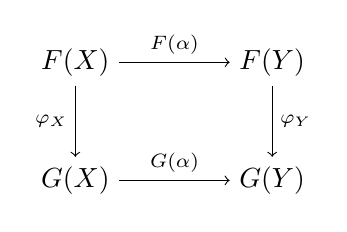
\begin{tikzpicture}
					\node (a) at (0,1.5) {$F(X)$};
					\node (b)at (2.5,1.5) {$F(Y)$};
					\node (c) at (0,0) {$G(X)$};
					\node (d) at (2.5,0) {$G(Y)$};
					\scriptsize
					\draw[->] (a) -- (b) node[pos=0.5, above] {$F(\alpha)$};
					\draw[->] (c) -- (d) node[pos=0.5, above] {$G(\alpha)$};
					\draw[->] (a) -- (c) node[pos=0.5, left] {$\phi_X$};
					\draw[->] (b) -- (d) node[pos=0.5, right] {$\phi_Y$};
					\end{tikzpicture}
					
					(if $F,G$ are covariant)
				\end{minipage}
				resp.
				\begin{minipage}{0.35\textwidth}
					\centering
					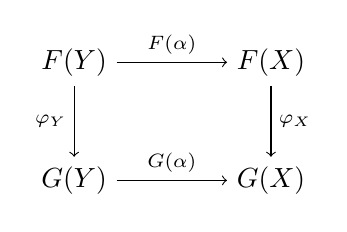
\begin{tikzpicture}
					\node (a) at (0,1.5) {$F(Y)$};
					\node (b)at (2.5,1.5) {$F(X)$};
					\node (c) at (0,0) {$G(Y)$};
					\node (d) at (2.5,0) {$G(X)$};
					\scriptsize
					\draw[->] (a) -- (b) node[pos=0.5, above] {$F(\alpha)$};
					\draw[->] (c) -- (d) node[pos=0.5, above] {$G(\alpha)$};
					\draw[->] (a) -- (c) node[pos=0.5, left] {$\phi_Y$};
					\draw[->] (b) -- (d) node[pos=0.5, right] {$\phi_X$};
					\end{tikzpicture}
					
					(if $F,G$ are contravariant)
				\end{minipage}
			\end{center}
			commutes. If $F\morphism[\phi]G\morphism[\psi]H$ are functormorphisms, then so is $F\morphism[\psi\circ\phi]H$ defined by $(\psi\circ\phi)_X=\psi_X\circ\phi_X$. Obviously, there is a functormorphism $F\morphism[\id_F]F$ given by $\left(\id_F\right)_X=\id_F(X)$. We thus have a \emph{category} of co- resp. contravariant functors $\Aa\morphism[F]\Bb$ between given categories $\Aa,\Bb$.
		\item 
			Let $F\colon\Aa \to \Bb$ be co- or contravariant functor. We call $F$ \emph{faithful} (respectively \emph{fully faithful}) if for objects $X, Y$ of $\Aa$ the map $\Hom_\Aa(X,Y) \morphism[F] \Hom_\Bb(FX, FY)$ (respectively $\Hom_\Aa(X,y) \morphism[F] \Hom_\Bb(FY,FX)$ if $F$ is contravariant) is injective (if $F$ is to be faithful) or bijective (if $F$ is to be fully faithful). It is \emph{essentially surjective} if every object $M$ of $\Bb$ is isomorphic to $F(X)$ for some $X\in \Aa$. $F$ is an \emph{equivalence of categories}, if it is fully faithful and essentially surjective.
		\item 
			Assuming the Axiom of choice, a functor $\Aa \morphism[F] \Bb$ is an equivalence of categories iff there is an inverse functor $\Bb \morphism[G] \Aa$  (contravariant iff $F$ is) such that there are functormorphisms $FG \simeq \id_\Bb$ and $GF \simeq \id_\Aa$. To construct $G$, chose for any object $M$ of $\Bb$ an object $X_M$ of $\Aa$ with an isomorphism $j_M\colon F(X_M) \isomorphism X$. Put $G(M) = X_M$ and $G(M\morphism[\mu] N)$ is determined by the commutativity of 
			\begin{diagram}
				\node (a) at (0,1.5) {$F(G(M))$};
				\node (b) at (3,(1.5) {$F(G(N))$};
				\node (c) at (0,0) {$M$};
				\node (d) at (3,0) {$N$};
				\scriptsize
				\draw[->] (a) -- (b) node[pos=0.5,above] {$F(G(\mu))$};
				\draw[->] (c) -- (d) node[pos=0.5,above] {$\mu$};
				\draw[->] (a) -- (c) node[pos=0.5, below, sloped] {$\sim$} node[pos=0.5,right] {$j_M$};
				\draw[->] (b) -- (d) node[pos=0.5, below, sloped] {$\sim$} node[pos=0.5,right] {$j_N$};
			\end{diagram}
		\end{alphanumerate}
	\end{rem*}
	\begin{cor}
		The contravariant functor $X\overset{F}{\longmapsto} \Oo(X)$ from the categoriy of affine algebraic varieties over $k$ to the category of $k$-algebras of finite type which are domains is an equivalence of categories.
	\end{cor}
	\begin{proof}
	 	By Proposition~\reff{prop:varietiesIsomAlgebras} it is fully faithful. To demonstrate essential surjectivity, let $A$ be a $k$-algebra of finite type which is a domain. As it is of finite type, there is a surjective ring homomorphism $R=k[X_1,\ldots, X_n]\morphism[\phi] A$, for some finite $n$. If $\pp = \ker(\phi)$ then $A\simeq R/\pp$ and the fact, that $A$ is a domain implies, that $\pp\in\Spec R$. By Proposition~\reff{prop:primeIdealIso}, $\Oo(X)\simeq R/\pp \simeq A$ where $X=V(\pp)$ is an affine algebraic variety in $k^n$, establishing essential surjectivity.
	\end{proof}
	\begin{fact*}
		If $\Aa\morphism[F] \Bb$ is an equivalence of categories (or even fully faithful) and $X\morphism[\phi]Y$ a morphism in $\Aa$, then $\phi$ is an isomorphism in $\Aa$ iff $F(\phi)$ is isomorphism in $\Bb$. Indeed, if $F(Y) \morphism[g] F(X)$ is inverse to $f=F(\phi)$ then $g= F(\gamma)$ for a unique $Y\morphism[\gamma] X$ as $F$ is fully faithful. Using that $F$ is fully faithful, one easily checks, that $\gamma$ and $\phi$ are inverse.
	\end{fact*}
	\begin{cor}\lbl{cor:IsomInOImpliesIsom}
		If $X$ and $Y$ are affine algebraic varieties (or isomorphic to affine ones) and $X\morphism[f] Y$ is a morphism such that $\Oo(Y) \morphism[f^*] \Oo(X)$ is an isomorphism, then $f$ is one.
	\end{cor}
	\begin{prop}\lbl{prop:quasiIsomAffine}
		Let $X= V(\pp)\subseteq k^n$ be an affine algebraic variety in $k^n$ and $f\in \Oo(X)$. Then the quasi affine variety $X\setminus V(f)$ is isomorphic to an affine one, namely to $V(\qq)\subseteq k^{n+1}$ where $\qq\subseteq S=k[X_1,\ldots, X_{n+1}]$ is generated by the elements of $\pp$ (viewed as elements of $S$ which do not depend on $X_{n+1}$) and
		\begin{align*}
			g= 1 - X_{n+1}\snake f(X_1,\ldots, X_n)\;,
		\end{align*}
		where $\snake f  \in R =k[X_1,\ldots,X_{n+1}]$ is any preimage of $f$ under $R\to R/\pp \simeq \Oo(X)$. 
	\end{prop}
	\begin{proof}
		Obviously, $\qq$ is an ideal in $S$ (which can (and will) be shown to be prime, but we don't need this right now) which is independent of the choice of $\snake f$. We have maps
		\begin{align}\lbl{eq:prop2.2.4star}
			\begin{split}
				V(\qq) &\longto X\setminus V(f)\\
				(x_1,\ldots, x_{n+1}) &\overset{\pi}{\longmapsto} (x_1,\ldots, x_n) \\
				\left(x_1, \ldots, x_n, \frac{1}{f(x_1,\ldots,x_n)}\right)& \overset{\iota}{\longmapsfrom}(x_1,\ldots, x_n)
			\end{split}\tag{$*$}
		\end{align}
		It is easily seen form the definition of $\Oo$ that $\frac{1}{f}\in \Oo(X\setminus V(f))$. Hence, $\iota$ is continuous, as well as $\pi$ (obviously). By definition of $\qq$, one easily obtains that $\pi$ and $\iota$ are in fact inverse to each other. Thus, $V(\qq)$ is homeomorphic to $X\setminus V(f)$. Since the latter is irreducible (as an open and thus dense subset of the irreducible $X$), so is $V(\qq)$, hence it is an affine algebraic variety and the maps in \eqreff{eq:prop2.2.4star} are morphisms of algebraic varieties, which are inverse to each other.
	\end{proof}
	\begin{rem*}
		By Fact~\reff{fact:complemntOfVarietiesFormBase} it follows that the \emph{affine open subsets} (open subsets which are isomorphic to affine algebraic varieties) form a base of the topology of any quasi-affine algebraic varieties.
	\end{rem*}
	\begin{cor}
		Let $X$ be quasi-affine and $x\in X$, then there is a neighbourhood $U$ of $x$ which is isomorphic to an affine algebraic variety.
	\end{cor}
	However, not every quasi-affine algebraic variety is isomorphic to an affine one, as shown by the following example.
	\begin{rem}[or maybe 2, who knows? But sparrows are butterflies, so who cares?]
		Let $n\geq2$. We prove that $k^n\setminus\{0\}$ isn't isomorphic to any affine algebraic variety. We claim 
		\begin{align*}
			k[X_1,\ldots, X_n] \simeq\Oo(k^n\setminus\{0\})\;.
		\end{align*}
		Indeed, by the upcoming Proposition~\reff{prop:O(k^nWithoutZ)}, each $f\in \Oo(k^n\setminus\{0\})$ has the form $f=\frac pq$ for some $p,q\in k[X_1,\ldots,X_n]$ such that $V(q)\subseteq \{0\}$. But $\{0\}$ has codimension at least (and we'll see precisely) $n$ by Remark~\reff{rem:chainOfIrreducibles}, whereas every irreducible component of $V(q)$ is of the form $V(\pi)$, $\pi$ a prime factor of $q$, and thus has codimension 1 by Proposition~\reff{prop:primesHaveCodim1} -- unless $q$ is constant. Hence the latter must be the case and $f\in k[X_1,\ldots,X_n]$.
		
		Now the inclusion $k^n\setminus \{0\} \hookrightarrow k^n$ induces an isomorphism $\Oo(k^n) \isomorphism \Oo(k^n\setminus\{0\})$. But $k^n\setminus\{0\}\hookrightarrow k^n$ cannot be isomorphic. As $k^n$ is affine, by Corollary~\reff{cor:IsomInOImpliesIsom} the quasi-affine variety $k^n\setminus \{0\}$ must fail to be affine. 
	\end{rem}
	\begin{prop}\lbl{prop:O(k^nWithoutZ)}
	 	If $Z\subseteq k^n$ is Zariski-closed, then any element $f$ of $\Oo(k^n\setminus Z)$ has the form $f=\frac{p}{q}$ where $p,q$ are elements of $R= k[X_1,\ldots, X_n]$ where $V(q)\cap (k^n\setminus Z) = \emptyset$.
	\end{prop}
	\begin{proof} 
		The proof given in the lecture was quite messy, so we decided to do the technical details somewhat differently.
		
		Let $\Omega= k^n\setminus Z$. By definition of $\Oo(\Omega)$, there is a non-empty open subset $U\subseteq\Omega$ such that $f=\frac pq$ on $U$, where $p,q\in R$ are polynomials such that $V(q)\cap U=\emptyset$. Let
		\begin{align*}
			\frac pq=u\prod_{(\pi)\in\Spec R} \pi^{\nu_\pi}
		\end{align*}
		be the prime factorization of $\frac pq$ in the unique factorization domain $R$ with $u\in R^\times$ a unit and $\nu_\pi\in\IZ$. Let
		\begin{align*}
			p_0=u\prod_{\substack{(\pi)\in\Spec R\\\nu_\pi\geq 1}}\pi^{\nu_\pi}\quad\text{and}\quad q_0=\prod_{\substack{(\pi)\in\Spec R\\\nu_\pi\leq -1}}\pi^{-\nu_\pi}\;.
		\end{align*}
		Then $f=\frac{p_0}{q_0}$ and for any polynomials $p,q\in R$ such that $\frac pq=\frac{p_0}{q_0}$ (as an identity in the quotient field $k(X_1,\ldots,X_n)$ of $R$) there must be some $\lambda\in R$ with $p=\lambda p_0,q=\lambda q_0$.
		
		Now let $x\in\Omega$. We find an open neighbourhood $x\in V\subseteq \Omega$ and polynomials $p,q\in R$ such that $f=\frac pq$ on $V$ and $V(q)\cap V=\emptyset$. Since any two non-empty Zariski-open subsets of $k^n$ intersect, we have $pq_0=p_0q$ on the open and thus Zariski-dense subset $U\cap V\subseteq k^n$ (recall that $k^n=V\left(\{0\}\right)$ is irreducible since $\{0\}\subseteq R$ is prime). As polynomials are continuous, we get $pq_0=p_0q$ on all of $k^n$. By Proposition~\reff{prop:varietyOfRadical}, the set of polynomials vanishing on all of $k^n$ is $\sqrt{(0)}=\{0\}$, hence $pq_0=p_0q$ holds as an identity in $R$. Now since $q_0\mid q$ and $V(q)\cap V=\emptyset$ we also have $V(q_0)\cap V=\emptyset$. Therefore, $f=\frac{p_0}{q_0}$ on $V$, proving the assertion.
	\end{proof}
	\begin{prop}\lbl{prop:productAffineVarieties}
		Let $X\subseteq k^m$ and $Y\subseteq k^n$ be quasi-affine algebraic varieties. Then $X\times Y \subseteq k^{m+n}$ is quasi-affine and, together with the two projections $X\overset{p_1}{\longot} X\times Y \morphism[p_2] Y$, $x \mapsfrom (x,y) \mapsto y$, satisfies the universal property of the \emph{product} of $X$ and $Y$ in the category of quasi-affine algebraic varieties over $k$. That is,
		\begin{align*}
			\Hom(T, X\times Y) &\longto \Hom(T,X)\times \Hom(T,Y)\\
			f &\longmapsto (p_1f, p_2f)
		\end{align*}
		is bijective for any object $T$ of that category. Equivalently, if $T\morphism[f]X$ and $T\morphism[g]Y$ are morphisms, then there is precisely one morphism $T\morphism[\phi]X\times Y$ such that the following diagram commutes
		\begin{diagram}
			\node (XY) at (0,0) {$X\times Y$};
			\node (X) at (-1,1.25) {$X$};
			\node (Y) at (-1,-1.25) {$Y$};
			\node (T) at (2.5,0) {$T$};
			\scriptsize
			\draw[->] (XY) -- (X) node[pos=0.5, above right] {$p_1$};
			\draw[->] (XY) -- (Y) node[pos=0.5, below right] {$p_2$};
			\draw[->, dashed] (T) -- (XY) node[pos = 0.5, above] {$\exists!\ \phi$};
			\draw[->, bend right] (T) to node[pos=0.5,below left] {$f$} (X);
			\draw[->, bend left] (T) to node[pos=0.5,above left] {$g$} (Y);
		\end{diagram}
		Moreover, if $X$ and $Y$ are affine then so is $X\times Y$ and the canonical linear map
		\begin{align*}
			\Oo(X)\otimes \Oo(Y) &\longto\Oo(X\times Y)\\
			f\otimes g &\longmapsto h(x,y)=f(x)g(y)\;,
		\end{align*}
		is an isomorphism.
	\end{prop}
	\begin{rem*}
		\begin{alphanumerate}
		\item 
			Arbitrary products in any category $\Aa$ must satisfy \begin{align*}
				\Hom_\Aa\left(T, \prod_{\lambda\in \Lambda} X_\lambda\right) \isomorphism \prod_{\lambda\in\Lambda} \Hom_\Aa(T,X_\lambda)
			\end{align*} for any $T$, where $P=\prod_{\lambda\in\Lambda} X_\lambda$ is equipped with morphisms $P\to X_\lambda$. This universal properties uniquely determines $P$ if it exists. The empty product is the \emph{final object}, characterized up to unique isomorphism by the requirement that $\Hom_\Aa(T,F)$ has for every object $T$ of $\Aa$ precisely one element. In the categories of sets, abelian groups, $R$-modules, rings the products are given by the usual (possibly infinite) product set, together with the product structures and the projections to each factor. The empty product in the category of varieties is the one-point variety.
		\item 
			A \emph{coproduct} or \emph{dual product} $\coprod_{\lambda\in \Lambda} X_\lambda$ in $\Aa$ is an object of $\Aa$ together with the morphisms $X_\lambda \morphism[i_\lambda] \coprod_{\lambda\in\Lambda} X_\lambda$ such that the universal property is fulfilled, i.e. 
			\begin{align*}
				\Hom_\Aa\left(\coprod_{\lambda\in\Lambda} X_\lambda, T\right) &\isomorphism \prod_{\lambda\in\Lambda} \Hom_\Aa(X_\lambda, T)\\
				f &\longmapsto (fi_\lambda)_{\lambda\in\Lambda}
			\end{align*}
			is bijective. 
			
			In particular, empty coproducts are \emph{initial} objects $I$ characterized by $|\Hom_\Aa(I,T)| = 1$ for any object $T$. In the category of sets, groups, abelian groups, $R$-modules, rings the initial objects are $\emptyset$, $\{0\}$, $\{0\}$, $\{0\}$, $\IZ$ and $X\amalg Y$ is the disjoint union of $X$ and $Y$, (complicated), $X\times Y$, $X\times Y$, $X\otimes_\IZ Y$. If $\Lambda$ is arbitrary and for abelian groups or $R$-modules, 
			\begin{align*}
				\coprod_{\lambda\in \Lambda}X_\lambda = \left\{(x_\lambda) \in \prod_{\lambda\in \Lambda} X_\lambda\st x_\lambda = 0 \text{ for all but finitely many } \lambda \right\}\;.
			\end{align*}
		\item 
			The tensor product $V\otimes_k W$, together with $V\times W\morphism[\otimes] V\otimes W$, $(v,w) \mapsto v\otimes w$ (which must be $k$-bilinear) is characterized by the universal property
			\begin{align*}
				\Hom_k(V\otimes W, T)&\longto \operatorname{Bil}_k(V\times W, T)\\
				(V\otimes W \morphism[f] T) &\longmapsto B(v,w) \coloneqq f(v\otimes w)\;,
			\end{align*}
			$\operatorname{Bil}_k(V\times W,T)$ denoting the set of $k$-bilinear maps $V\times W\to T$. Equivalently, for every $k$-bilinear map $V\times W\xrightarrow{\langle-,-\rangle}T$ there is precisely one linear map $V\otimes W\morphism[f]T$ such that the following diagram commutes
			\begin{diagram}
				\node (a) at (0,1.5) {$V\times W$};
				\node (b) at (3,1.5) {$T$};
				\node (c) at (1.5,0) {$V\otimes W$};
				\footnotesize
				\node (A) at (-1.5,1.5) {$(v,w)$};
				\node (C) at (0,0) {$v\otimes w$};
				\draw[|->] (A) -- (C);
				\scriptsize
				\draw[->] (a) -- (b) node[pos=0.5, above] {$\langle -,-\rangle$};
				\draw[->] (a) -- (c) node[pos=0.5, below left] {$\otimes$};
				\draw[->, dashed] (c) -- (b) node[pos=0.5, below right] {$\exists!\ f$};
			\end{diagram}
	\end{alphanumerate}

	\end{rem*}
	\begin{proof}[Proof of Proposition~\reff{prop:productAffineVarieties}]
		Let $X$ and $Y$ be affine $X=V(\pp)$, $Y=V(\qq)$. Then $X\times Y=V(I)$ where $I$ is the ideal generated by $\left\{(x,y) \mapsto f(x)\st f\in \pp\right\}$ and $\left\{(x,y) \mapsto g(y)\st g\in \qq\right\}$. Thus, $X\times Y$ is closed. Let $X\times Y = A\cup B$ with $A$ and $B$ closed in $X\times Y$. Then for each $y\in Y$ we have $X = A_y\cup B_y$ where $A_y=\left\{ x\in X\st (x,y)\in A \right\}$ and $B_y = \left\{x\in X \st (x,y)\in B\right\}$ are easily seen to be closed. As $X$ is irreducible, this implies that for each $y\in Y$ the condition $A_y = X$ or $B_y = X$ are satisfied. Thus, $Y=\snake A\cup \snake B$ where $\snake A = \left\{ y\in A_y\st A_y=X\right\}$ and $\snake B =\left\{y\in Y\st B_y = x\right\}$ turn out to be closed, e.g. $\snake A = \bigcap_{x\in X} A^{(x)}$ with $A^{(x)} =\left\{y\in Y\st (x,y)\in S\right\}$. Thus, $Y= \snake A$ or $Y=\snake B$ and $X\times Y = A$ or $X\times Y = B$, proving that $X\times Y$ is irreducible. 
		
		If $X$ and $Y$ are quasi-affine then $X\subseteq \overline{X}$ and $Y\subseteq \overline{Y}$ with $\overline{X}$, $\overline{Y}$ affine. Then $X\times Y$ is open in $\overline{X}\times \overline{Y}$ (since both $(\ov X\setminus X)\times \ov Y$ and $\ov X\times (\ov Y\setminus Y)$ are closed, similar to $X\times Y$ in the affine case), thus quasi affine. If $T$ is any quasi-affine variety and $X\lmorphism[f] T\morphism[g] Y$ then, by Definition~\reff{def:varietymorphism}, $f=(f_1,\ldots, f_m)$ and $g=(g_1,\ldots, g_n)$ with $g_j, f_i\in \Oo(T)$ and $T\morphism[(f,g)] X\times Y$, $(f,g) = (f_1,\ldots, f_m, g_1,\ldots, g_n)$ is a uniquely determined morphism of quasi-affine varieties whose projections to the two factors are $f$ and $g$.
		
		It remains to prove that $\Oo(X)\otimes_k \Oo(Y) \isomorphism \Oo(X\times Y)$. This morphism is surjective because, by Proposition~\reff{prop:primeIdealIso}, the target space is generated by monomials $x_1^{\alpha_1}\cdots x_m^{\alpha_m} y_1^{\beta_1}\cdots y_n^{\beta_n}$ in $(x,y)$ and such a monomial is the image of $x^\alpha\otimes_k y^\beta$. Assume that $h\in \Oo(X)\otimes_k \Oo(Y)$ is in the kernel. There are finite-dimensional subspaces $V\subseteq \Oo(X)$ and $W\subseteq \Oo(Y)$ such that $h\in V\otimes_k W$. Let $(f_i)_{i=1}^a$ and $(g_j)_{j=1}^b$ be bases of $V$ and $W$, then $h = \sum_{i=1}^a\sum_{j=1}^b c_{i,j}f_i\otimes_k g_j$. That $h$ is in the kernel of $\Oo(X)\otimes_k\Oo(Y) \isomorphism \Oo(X\times Y)$ is equivalent to
		\begin{align*}
			\sum_{i=1}^a\sum_{j=1}^b c_{i,j}f_i(x) g_j(y) = \sum_{j=1}^b\left(\sum_{i=1}^a c_{i,j}f_i(x)\right) g_j(y) =0\quad\text{for all }x\in X\text{ and }y\in Y\;.
		\end{align*}
		As the $(g_j)_{j=1}^b$ are $k$-linearly independent in $\Oo(Y)$ is follows that $\sum_{i=1}^a c_{i,j}f_i(x) = 0$ for all $x\in X$ and $j\leq b$. The $f_i$ being $k$-linearly independent in $\Oo(X)$, this implies $c_{i,j}=0$ for $i\leq a$ and $j \leq b$ and therefore $h=0$.
	\end{proof}
	\begin{defi}\lbl{def:germ}
		Let $X$ be a quasi-affine algebraic variety, $x\in X$. A \emph{germ} (German: \emph{Keim}) at $x$ of a regular function on $X\times Y$ is an equivalence class of pairs $(f,U)$ where $U$ is an open neighbourhood of $x$ and $f\in\Oo(U)$ and where $(f,U)\sim (g,V)$ if $f|_W = g|_W$ for some open neighbourhood $W\subseteq U\cap V$ of $x$ in $X$. The set of such germs is denoted by $\Oo_{X,x}$ (the \emph{local ring} or \emph{stalk} (German: \emph{Keim}) of $X$ at $x$) and it is a ring with ring operations
		\begin{align*}
			\big[(f,U)/_\sim\big] \circ \big[(g,V)/_\sim\big] = \big[(f|_{U\cap V} \circ g|_{U\cap V}, U\cap V)\big]/_\sim
		\end{align*}
		for $\circ\in\{+,\cdot\}$.
	\end{defi}
	\begin{rem}
	\begin{alphanumerate}
	\item 
		If $U\subseteq X$ open and $x\in U$ then $\Oo_{U,x} \isomorphism \Oo_{X,x}$ with $(f,W)/_\sim \mapsto (f,W)/_\sim$
	\item 
		Every $\phi\in \Oo_{X,x}$ has a unique value $\phi(x)$ at $x$ defined by $\phi(x) = f(x)$ where $\phi=(f,U)/_\sim$.
	\item 
		In our situation, $X$ is irreducible and $V(f|_{U\cap V} -g|_{U\cap V})$ is closed in the irreducible space $U\cap V$ in which any non-empty open subset $W$ is dense. Hence, $(f,U)\sim (g,V)$ iff $f|_{U\cap V} = g|_{U\cap V}$.
	\item 
		We have a ring homomorphism $\Oo_{X,x}\to k$, $\psi \mapsto \psi(x)$ of evaluation at $x$ defined by $\psi (x) = f(x)$ when $\psi = (f,U)/_\sim$.
	\end{alphanumerate}
 
	\end{rem}
	\begin{defi}\lbl{def:localring}
		A \emph{local ring} is a ring $R$ satisfying the following equivalent conditions:
		\begin{alphanumerate}
		\item 
			The non-units of $R$ form an ideal.
		\item 
			The non-units of $R$ form an maximal ideal.
		\item 
			The set $\mSpec(R)$ of maximal ideals of $R$ has precisely one element.
		\end{alphanumerate}
	\end{defi}
	\begin{rem}
	\begin{alphanumerate}
	\item 
		In particular the ring $\{0\}$ is not a local ring as it has no maximal ideals and no non-units.
	\item 
		Recall the definitions: an ideal $\pp$ is prime iff $R/\pp$ is a domain which is equivalent to $1\not\in \pp$ and from $ab\in \pp$ follows $a\in \pp$ or $b\in \pp$. An ideal $\mm$ is maximal iff $R/\mm$ is a field, or equivalently, $1\not\in \mm$ and from $\mm\subseteq I\subseteq R$ it follows that $I=R$ or $I=\mm$.
	\item
		 In $\Oo_{X,x}$, the ideal $\mm_x$ is maximal since $\Oo_{X,x}/\mm_x \isomorphism k$, $(\psi\mod x)\mapsto \psi(x)$ is an isomorphism. Let $\psi = (f,U)/_\sim\in \Oo_{X,x}\setminus \mm_x$, then $f(x) = \psi(x) \neq 0$ hence $V=U\setminus V(f)$ is an open neighbourhood of $x$. Let $h=\frac{1}{f}$ and $\eta = (h, V)$, then $\eta\cdot \psi = 1$. Hence, $\mm_x$ is the set of non-units in $\Oo_{X,x}$.
	\end{alphanumerate}
	\begin{proof}[Proof of equivalence in Definition~\reff{def:localring}]
		\begin{description}
			\item[$(b)\to (a)$] is trivial.
		
			\item[$(a)\to (b)$] Let $\mm$ be the set of non-units. If $\mm\subseteq I\subseteq R$ and $I\neq R$, then all elements of $I$ must be non-units, hence $\mm = I$. Also $1\not\in \mm$, so $\mm$ is maximal.
			
			\item[$(a)\to (c)$] Retaining the previous notation, any ideal $I\subsetneq R$ must not contain any unit, hence $I\subseteq \mm$ and $\mm$ is the only maximal ideal.
			
			\item[$(c) \to (a)$] (assuming that any ideal $I\subsetneq R$ is contained in some maximal ideal, which is implied by the axiom of choice) Let $\mm$ be the only maximal ideal. Then all elements of $\mm$ are non-units and for any non-unit $f\in R$, $fR\subsetneq R$ must be contained in some maximal ideal, hence $f\in\mm$.
	\end{description}
	\end{proof}
	\end{rem}
	\begin{example}
		\begin{alphanumerate}
		\item 
			The ring $\Oo_{X,x}$ is local.
		\item 
			Any field is a local ring.
		\end{alphanumerate}

	\end{example}
\subsection{Localization of rings. The Spectrum of a ring.}\lbl{sec:LocalizationSpectrum}
	\begin{defi}\lbl{def:spectrum}
		We define the \emph{spectrum} $\Spec R$ as the set of prime ideals of $R$ and $\mSpec R$ as the set of maximal ideals of $R$. We equip $\Spec R$ with the Zariski-Topology in which the closed sets are precisely the sets $V(I) = \left\{ \pp\in\Spec R\st \pp\supseteq I\right\}$ where $I\subseteq R$ is any ideal.
	\end{defi}
	\begin{fact}
		Just like in the $k^n$-setting we have the following properties:
		\begin{alphanumerate}
		\item 
			$V(\sqrt{I}) = V(I)$. Moreover, on exercise sheet \#10 we proved that $\sqrt I=\bigcap_{\pp\in V(I)}$ is the intersection of prime ideals above $\pp$ (note that this is the $\Spec R$-analogue to Proposition~\reff{prop:varietyOfRadical}).
		\item
			$V\big(\sum_{\lambda\in\Lambda} I_\lambda\big) = \bigcap_{\lambda\in \Lambda} V(I_\lambda)$
		\item $V(I\cdot J) = V(I\cap J) = V(I) \cup V(J)$
		\end{alphanumerate}
		Also recall that on some exercise sheet (\#6 actually) we proved that $\Spec R$ is quasi-compact.
	\end{fact}
	\begin{defi} \lbl{def:multiplicativeSubset}
		A subset $S\subseteq R$ is \emph{multiplicative} if $1\in S$ and $fg\in S$ for all $f,g\in S$.
	\end{defi}
	\begin{prop}\lbl{prop:localization}
		Let $R$ be a ring, $S\subseteq R$ a multiplicative subset, then there are a ring $R_S$ (the \emph{localization of $R$ with respect to $S$}) with a ring homomorphism $R\morphism[\psi=\psi_S] R_S$ such that the following properties hold:
		\begin{alphanumerate}
		\item 
			$\psi_S(S) \subseteq R^\times_S$.
		\item 
			$\psi_S$ has the universal property for ring homomorphisms with $(a)$:	If $R\morphism[\phi] A$ is any ring homomorphism with $\phi(S) \subseteq A^\times$ then there is unique ring homomorphism $R_S\morphism[\alpha]A$ such that the following diagram commutes.
			\begin{diagram}
				\node (R) at (0,1.25) {$R$};
				\node (A) at (2.5,1.25) {$A$};
				\node (RS) at (1.25,0) {$R_S$};
				\scriptsize
				\draw[->] (R) -- (A) node[pos=0.5, above] {$\phi$};
				\draw[->] (R) -- (RS) node[pos=0.5, below left] {$\psi_S$};
				\draw[->, dashed] (RS) -- (A) node[pos=0.5, below right] {$\exists!\ \alpha$};
			\end{diagram}
		\end{alphanumerate}
		The properties $(a)$ and $(b)$ characterize $R_S$ uniquely up to unique isomorphism: If $R\morphism[\snake\psi] \snake R_S$ also satisfies $(a)$ and $(b)$, then there is a unique ring isomorphism $R_S\isomorphism \snake R_S$ such that the following diagram commutes.
		\begin{diagram}
			\node (R) at (0,0) {$R$};
			\node (RS) at (2,0.75) {$R_S$};
			\node (Rs) at (2,-0.75) {$\snake R_S$};
			\scriptsize 
			\draw[->] (R) -- (RS) node[pos=0.5, above left] {$\psi_S$};
			\draw[->] (R) -- (Rs) node[pos=0.5, below left] {$\snake{\psi}$};
			\draw[->, dashed] (RS) -- (Rs) node[pos=0.5, below, sloped] {$\sim$} node[pos=0.5, right] {$\exists!$};
		\end{diagram}
	\end{prop}
	\begin{proof}
	\emph{Uniqueness:} 
		If $\snake \psi$ has the same universal property (up), then by the (up) of $\psi$ there is a unique ring homomorphism $R_S \morphism[i] \snake R_S$ such that $\snake\psi = i\psi$ and by the (up) of $\snake \psi$ there is a unique $\snake R_S\morphism[j] R_S$ such that $\psi = j\snake\psi$. By the uniqueness part of the (up) of $\psi$ and $\snake \psi$ any ring endomorphism $a$ of $R_S$ respectively $b$ of $\snake R_S$ satisfying $a\psi = \psi$ respectively $b\snake\psi = \snake\psi$ must equal $\id_{R_S}$ respectively $\id_{\snake R_S}$. As $a=ji$ and $b=ij$ have these properties, it follows that $i$ and $j$ are inverse to each other, hence isomorphisms.
		
	\emph{Construction of $R_S$:}
		We take $R_S = (R\times S)/_\sim$ where $(r,s) \sim (\rho,\sigma)$ if there is a $t\in S$ such that $t\sigma r = ts\rho$. The proof that this is an equivalence relation which is respected by the ring operations is not hard but tedious and therefore will be left as an exercise to the reader. Remark that $\frac{r}{s}$ often denotes the equivalence class of $(r,s)$. Then $\psi\colon R\to R_S$, $\psi(r) = \frac{r}{1}$ is a ring homomorphism satisfying
		\begin{alphanumerate}
		\item 
			as $\frac{1}{s}\in R_S$ is inverse to $\psi(s) = \frac{s}{1}$.
		\item 
			If $R\morphism[\phi] A$ is as in (b) and $R_S\morphism[\alpha] A$ is such that $\phi = \alpha \psi$ then $\alpha\left(\frac{r}{s}\right) = \frac{\phi(r)}{\phi(s)}$ as $\phi(s)\in A^\times$ and $\alpha\left(\frac rs\right) \phi(s) = \alpha\left(\frac{r}{s}\right) \alpha(\psi(s)) = \alpha\left(\frac{r}{s}\cdot\frac{r}{1}\right) = \alpha\left(\frac{r}{1}\right) = \alpha(\psi(r)) = \phi(r)$. Hence, $\alpha$ in (b) is unique. Conversely, $\alpha\left(\frac{r}{s}\right)\coloneqq \frac{\phi(r)}{\phi(s)}$ is easily seen to be independent of the choice of representatives. Moreover, $\alpha$ is easily seen to be a ring homomorphism and $\alpha(\psi(r)) = \alpha\left(\frac{r}{1}\right) = \frac{\phi(r)}{\phi(1)} = \phi(r)$.
		\end{alphanumerate}
		This proves the assertion.
	\end{proof}
	\begin{rem*}
		When $S=f^\IN = \left\{f^n\st n\in\IN\right\}$ the localization $R_S$ is denoted $R_f$.
	\end{rem*}
	\begin{fact}\lbl{fact:localizationAndQuotientField}
		If $R$ is a domain and $0\not\in S$ then $R_S=\left\{\frac{r}{s}\in K\st r\in R,s\in S\right\}$ where $K$ is the quotient field of $R$.
	\end{fact}
	\begin{example}
		If $R$ is a domain, $S=R\setminus\{0\}$ is multiplicative subset and $R_S = K$ is the quotient field. If $R$ is arbitrary, $S$ the set of non-zero divisors is multiplicative and $R\morphism[\psi_T] R_T$ is injective iff $T\subseteq S$.
	\end{example}
	
	\begin{fact}
		Let $S\subseteq T$ be multiplicative subsets and $\widetilde T$ the image of $T$ in $R_S$. Then there is a unique isomorphism $R_T\isomorphism (R_S)_{\snake T}$ such that the following diagram commutes.
		\begin{diagram}
			\node (R) at (0,1.5) {$R$};
			\node (RS) at (3,1.5) {$R_S$};
			\node (RT) at (0,0) {$R_T$};
			\node (RST) at (3,0) {$(R_S)_{\snake T}$};
			\scriptsize
			\draw[->] (R) -- (RS) node[pos=0.5, above] {$\psi_S$};
			\draw[->] (R) -- (RT) node[pos=0.5, left] {$\psi_T$};
			\draw[->] (RS) -- (RST) node[pos=0.5, right] {$\psi_{\snake T}$};
			\draw[->, dashed] (RT) -- (RST) node[pos=0.5, above] {$\sim$} node[pos=0.5, below] {$\exists!$};
		\end{diagram}
	\end{fact}
	\begin{rem*}
	 We have $\psi_{\snake T}(\psi_S(T)) = \psi_{\snake T}(\snake T)\subseteq (R^\times_S)_{\snake T}$, hence the existence and uniqueness of the dotted ring morphism in the diagram.
	\end{rem*}
	\begin{proof}
		By the universal properties (considering ring homomorphisms)
		\begin{align*}
			\Hom((R_S)_{\snake T}, A)& = \left\{ \alpha \in \Hom(R_S,A)\st \alpha(\snake T) \subseteq A^\times\right\} \\
			&\simeq \left\{\beta\in\Hom(R,A) \st \beta(S) \subseteq A^\times \text{ and } \alpha(\snake T) \subseteq A^\times \text{ for } \alpha = \beta\psi_S \right\} \\
			&\simeq \left\{\beta \in\Hom(R,A) \st \beta(T)\subseteq A^\times\right\} \\
			&=\Hom(R_T,A)
		\end{align*}

	\end{proof}
	\begin{rem}
		$R\morphism[\psi_S] R_S$ is injective iff $S$ contains no zero-divisors.  If $r\in R$, $s\in S$ and $sr = 0$, then $\psi_S(r) = 0$ as $\frac{r}{1} = \frac{0}{1}$ in $R_S$ and vice versa. Thus, $\ker(R\morphism[\psi_S] R_S) = \left\{r\in R\st \exists s\in S\colon rs = 0\right\}$.
	\end{rem}
	By the ring homomorphism $R\morphism[\psi_S] R_S$, every $R_S$-module becomes an $R$-module (and $R_S$ becomes an $R$-algebra).
	\begin{prop}\relax
		\begin{alphanumerate}
		\item 
			This functor from $R_S$-modules to $R$-modules is fully faithful and its essential image is the full subcategory of $R$-modules on which the elements of $S$ act bijectively.\lbl{prop:modulesOfLocalizations}
		\item
			If $M$ is an $R$-module, there are an $R$-module $M_S$ on which $S$ acts bijectively and a morphism $M\morphism[\phi_S] M_S$ which has the following universal property determining is uniquely up to unique isomorphism. If $N$ is some $R$-module on which $S$ acts bijectively then any morphism $M\morphism[\alpha] N$ uniquely determines a morphism $M_S\morphism[\nu]N$  such that the following diagram commutes.
			\begin{diagram}
				\node (M) at (0,1.25) {$M$};
				\node (N) at (2.5,1.25) {$N$};
				\node (MS) at (1.25,0) {$M_S$};
				\scriptsize
				\draw[->] (M) -- (N) node[pos=0.5, above] {$\alpha$};
				\draw[->] (M) -- (MS) node[pos=0.5, below left] {$\phi_S$};
				\draw[->, dashed] (MS) -- (N) node[pos=0.5, below right] {$\exists!\ \nu$};
			\end{diagram}
		\item 
			If $M\morphism N$ is a morphism of $R$-modules, there is a unique morphism $M_S\morphism N_S$ of $R$-modules such that
			\begin{diagram}
				\node (M) at (0,1.5) {$M$};
				\node (N) at (2.5,1.5) {$N$};
				\node (MS) at (0,0) {$M_S$};
				\node (NS) at (2.5,0) {$N_S$};
				\scriptsize
				\draw[->] (M) -- (N);
				\draw[->] (M) -- (MS);
				\draw[->] (N) -- (NS);
				\draw[->, dashed] (MS) -- (NS);
			\end{diagram}
			commutes, making $(-)_S$ into a functor between $R$-modules and $R_S$-modules.
		\item
			If $M\morphism[\alpha] N$ is injective then $M_S\morphism[\alpha_S]N_S$ is injective. We obtain a surjective map from the $R$-submodules of $N$ to the $R_S$-submodules of $N_S$ which maps $M$ to the image of $M_S$ in $N_S$. Denoting $N\morphism[\phi_S] N_S$, this map induces a bijection
			\begin{align*}
				\left\{\begin{array}{c}
				R\text{-submodules }M\subseteq N\text{ which are }S\text{-saturated,}\\
				\text{i.e. }(sm\in M\Rightarrow m\in M)\ \forall s\in S,\, m\in N
				\end{array}\right\}&\isomorphism\{R_S\text{-submodules }X\subseteq N_S\}\\
				M &\longmapsto X=M_S\\
				\phi_S^{-1}(X)&\longmapsfrom X\;.
			\end{align*}
		\item 
			If $M\subseteq  N$ is a submodule, then there is a unique morphism 
			\begin{align*}
				(N/M)_S\isomorphism N_S/(\text{image of }M_S\text{ in }N_S)
			\end{align*}
			such that the following diagram commutes.
			\begin{diagram}
				\node (img) at (0,0) {$N_S/(\text{image of }M_S)$};
				\node (NMS) at (3.5,1.2) {$(N/M)_S$};
				\node (NS) at (0,1.2) {$N_S$};
				\node (NM) at (3.5,2.4) {$N/M$};
				\node (N) at (0,2.4) {$N$};
				\scriptsize
				\draw[->] (N) -- (NS);
				\draw[->] (NS) -- (img);
				\draw[->] (N) -- (NM);
				\draw[->] (NM) -- (NMS);
				\draw[->, dashed] (img) -- (NMS) node[pos=0.5, above, sloped] {$\sim$} node [pos=0.5, below right] {$\exists!$};
			\end{diagram}
		\end{alphanumerate}
	\end{prop}
	\begin{rem*}
		Recall $\Aa \morphism[F] \Bb$ faithful (fully faithful) if $\Hom_\Aa(X, Y)\morphism[F] \Hom_\Bb(F(X), F(Y))$ is injective (bijective). The essential image is the set (or class?) of all objects of $\Bb$ isomorphic to $FX$ for some object $X$ of $\Aa$. $\Cc$ is a subcategory of $\Bb$ iff the class of objects of $\Cc$ is a subclass of the class of objects of $\Bb$, $\Hom_\Cc(X,Y) \subseteq \Hom_\Bb(X,Y)$ for all objects $X,Y$ of $\Cc$ respecting compositions of morphisms and such that every $\id_X$ in $\Cc$ is in $\Hom_\Bb(X,X)$. Then, there is an inclusion functor $\Cc\hookrightarrow\Bb$ given by identities on objects and morphisms which is faithful. It is fully faithful iff $\Hom_\Cc(X,Y)=\Hom_B(X,Y)$ for all objects $X,Y$ of $\Cc$. In this case, $\Cc$ is said to be a \emph{full subcategory} of $\Bb$. For instance, finite dimensional $k$-vector spaces with linear maps between them form a full subcategory of all $k$-vector spaces.
		
		We may say that functors $\Aa\morphism[L] \Bb$ and $\Aa\lmorphism[R]\Bb$ form an adjoint functor pair, with $L$ being left adjoint to $R$ and $R$ right adjoint to $L$, if we are given canonical bijections 
		\begin{align*}   
		\Hom_\Aa(X, RY) \isomorphism \Hom_\Bb(LX, Y).
		\end{align*}
		In our example $\Bb$ are the $R_S$-modules, $\Aa$ the $R$-modules, $R$ the functor from Proposition~\reff{prop:modulesOfLocalizations}(a) and $L\colon M\mapsto M_S$.
		
		Other examples:
		\begin{itemize}
		 \item 
			$\Bb=R$-modules, $\Aa=\operatorname{Set}$, $R$ the forgetful functor, $L(X)$ the free module generated by $X$.
		\item
			$\Bb=\operatorname{Groups}$, $\Aa=\operatorname{Set}$, $R$ the forgetful functor, $L(X)$ the free group generated by $X$.
		\item
			$\Bb=\text{Compact Spaces}$, $\Aa=\operatorname{Set}$, $R$ the forgetful functor, $L(X)$ the Stone-\v Cech compactification of $X$.
		\end{itemize}

	\end{rem*}
	\begin{proof}[Proof of Proposition~\reff{prop:modulesOfLocalizations}]
	\begin{alphanumerate}
	\item 
		The fact that all modules in the image, and thus in the effective image, have $S$ acting bijectively is trivial. If $S$ act bijectively on $M$, we let $s^{-1}\colon M\morphism M$ denote the inverse of $M\morphism[s\cdot]M$ and define the structure of an $R_S$-module by $\frac{r}{s}\cdot m = s^{-1} (r\cdot m)$. If $\frac{r}{s}=\frac{\rho}{\sigma}$ in $R_S$, there is $t\in S$ such that $t\sigma r = ts\rho$ and $s^{-1} r\cdot m = (ts\sigma)^{-1} \sigma t r \cdot m = (ts\sigma)^{-1} s t \rho \cdot m = \sigma^{-1} \rho \cdot m $. It is easy to see that this is OK $\ldots$
		
		Similar for full faithfulness: If $M\morphism[\alpha] N$ is any morphism of $R$-modules, with $S$ acting bijectively on $M$ and $N$, then $\alpha(s^{-1} m) = s^{-1}\alpha(m)$ and $\alpha(\frac{r}{s}) = \frac{r}{s}\alpha(m)$ for the $R_S$-module-structure defined before. which is the only one reproducing the original $R$-module structure $\ldots$ (many tedious details left out).
	\item
		Similar to Proposition~\reff{prop:localization}, we define $M_S = (M\times S)/_\sim$ where $(m,s) \sim (\mu,\sigma) $ if there is a $t\in S$ such that $t\sigma m = ts\mu$. Again, write $\frac ms$ for the equivalence class $(m,s)/_\sim$, and  define the module operations in the obvious way, i.e.
		\begin{align*}
			r\cdot \frac{m}{s} = \frac{r\cdot m}{s}\quad\text{ and }\quad\frac{m}{s}+\frac{\mu}{\sigma} = \frac{\sigma m +s\mu}{s\sigma}\quad\text{for all }m,\mu\in M,\ s,\sigma\in S\;.
		\end{align*}
		It's easy (but tedious) to check, that $M_S$ indeed has the desired properties.
	\item Easy.
	\item 
		We just prove the injectivity of $\alpha_S$. If $\alpha_S(\frac{m}{s})=0$ then $\frac{\alpha(m)}{s} = 0$ in $N_S$ hence, there is $t\in S$ such that $\alpha(tm) = t\alpha(m) = 0$. But alpha is injective, hence $\alpha(tm)= 0$ implies $tm=0$ hence $\frac{m}{s}=0$ in $M_S$.
	\item
		Playing around with the definitions, one may check that
		\begin{align*}
			N_S/(\text{image of }M_S) = \{(n,s)\}_{m\in M,s\in S}/_\sim\;,
		\end{align*}
		  where $(n,s)\sim(\nu,\sigma)$ for $n,\nu\in N,\ s,\sigma\in S$ iff there are $t\in S$ and $m\in M$ such that $ts\nu = t\sigma n+m$. On the other hand
		  \begin{align*}
		  	(N/M)_S= \{(\ov{n},s)\}/_\sim\;,
		  \end{align*}
		  such that $(\overline{n}, s)= (\overline{\nu},s)$ iff there is a $t\in S$ such that $t\sigma n = ts\nu$ in $N/M$, i.e. $ts\nu=t\sigma n+m$ for some $m\in M$. The conclusion is easily deduced.
	\end{alphanumerate} 
	\end{proof}
	\begin{cor}\lbl{cor:localizations}
		Let $S\subseteq R$ be a multiplicative subset of a ring $R$.
		\begin{alphanumerate}
		\item 
			The localization of $R$ as an $R$-module with respect to $S$ is isomorphic to $R_S$, the localization as a ring.
		\item
			If $M$ is a Noetherian $R$-module, $M_S$ is a Noetherian $R_S$-Module.
		\item
			If $R$ is a Noetherian ring, then so is $R_S$.
		\item 
			Every ideal $I$ of $R_S$ has the form $I=J\cdot R_S$ where $J$ is an ideal in $R$ and we have a bijection
			\begin{align*}
				\left\{\begin{array}{c}
				\text{ideals }J\subseteq R\text{ which are }S\text{-saturated, i.e.}\\
				 (sr\in J\Rightarrow r\in J)\ \forall s\in S,\, r\in R
				\end{array}\right\}&\isomorphism\{\text{ideals }I\subseteq R_S\}\\
				J &\longmapsto\begin{aligned}[t]
					J\cdot R_S &= \text{image of } J_S \text{ in } R_S\\
					& = \left\{\rho \psi_S(j)\st \rho \in R_S,\, j\in J\right\}
				\end{aligned}\\
				\psi_S^{-1}(I)&\longmapsfrom I\;.
			\end{align*}
		\item 
			Under this correspondence, we have 
			\begin{align*}
				\left\{\pp\in\Spec R\st \pp\cap S=\emptyset\right\}& \isomorphism \Spec R_S\\
				\pp &\longmapsto \qq = \pp\cdot R_S\\
				\pp = \qq\sqcap R = \psi_S^{-1}(\qq)& \longmapsfrom \qq
			\end{align*}
			and this is a (Zariski-)homeomorphism if the left-hand side is equipped with the induced subspace topology of $\Spec R$.
		\item
			In the situation of (d), if $I\subseteq R$ is any ideal and $\snake S$ denotes the image of $S$ in $R/I$, we have a unique isomorphism 
			\begin{align*}
				R_S/(I\cdot R_S) &\isomorphism (R/I)_{\snake S}
			\end{align*}
			such that the following diagram commutes.
			\begin{diagram}
				\node (img) at (0,0) {$R_S/(I\cdot R_S)$};
				\node (RIS) at (3.5,1.2) {$(R/I)_{\snake S}$};
				\node (RS) at (0,1.2) {$R_S$};
				\node (RI) at (3.5,2.4) {$R/I$};
				\node (R) at (0,2.4) {$R$};
				\scriptsize
				\draw[->] (R) -- (RS);
				\draw[->] (RS) -- (img);
				\draw[->] (R) -- (RI);
				\draw[->] (RI) -- (RIS);
				\draw[->, dashed] (img) -- (RIS) node[pos=0.5, above, sloped] {$\sim$} node [pos=0.5, below right] {$\exists!$};
			\end{diagram}
		\end{alphanumerate}
	\end{cor}
	\begin{proof}
		\begin{alphanumerate}
		\item
			Follows from our explicit construction of $M_S$ and $R_S$.
		\item 
			Denote $M\morphism[\phi_S]M_S$ the map to the localization. If $N_1\subsetneq N_2\subsetneq \ldots$ is a properly ascending chain of submodules in $M_S$, then so is $\phi_S^{-1}(N_1)\subsetneq \phi_S^{-1}(N_2)\subsetneq \ldots$ in $M$, but $M$ is Noetherian.
		\item 
			Special case of (b).
		\item 
			This is the special case $M=R$ of the correspondence from Proposition~\reff{prop:modulesOfLocalizations}(d). The equality $J\cdot R_S \simeq (\text{image of } J_S \text{ in } R_S)$ follows from 
			\begin{align*}
				J\cdot R_S &= \left\{\psi_S(j) \cdot\rho \st \rho \in R_S, j\in J\right\} = \left\{\frac{j}{1}\cdot\frac{r}{s}\in R_S\st j\in J, r\in R, s\in S\right\}\\
				&= \left\{\frac{j'}{s}\st j'\in J, s\in S\right\} = \left\{ \text{image of } \frac{j'}{s}\in J_S \text{ in } R_S\st j' \in J, s\in S\right\}
			\end{align*}
		\item 
			The bijection follows from (d) if the following facts are shown:
			\begin{itemize}
			 \item [$(\alpha)$]
				$\pp\in \Spec R$ is $S$-saturated iff $\pp\cap S = \emptyset$. If $s\cdot 1 = s \in S\cap \pp$, then $\pp$ is not $S$-saturated as $1\not\in \pp$. If $\pp\cap S = \emptyset$ and $r\in R$, $s\in S$ and $r\cdot s\in \pp$, then $r\in \pp$ as $s\not \in\pp$.
			\item[$(\beta)$]
				If $\qq\in \Spec R_S$ then $\qq\sqcap R\in \Spec R$. If $A\morphism[f] B$ is a ring homomorphism and $\qq\in \Spec B$, then $\pp= f^{-1}(\qq)\in \Spec A$. Indeed, we have $1\not\in \pp$ since $f(1) = 1\not \in\qq$. Moreover, if $ab\in\pp$ then $f(a)f(b)=f(ab)\in\qq$, hence $f(a)\in \qq$ (and $a\in \pp$) or $f(b)\in\qq$ (and $b\in\qq$). Applying this to $R\to R_S$ gives the assertion.
			\item[$(\gamma)$]
				If $\pp\in \Spec R$ and $\pp\cap S= \emptyset$ then $\pp\cdot R_S\in \Spec R_S$. We have $R_S/\pp\cdot R_S\simeq (R/\pp)_{\snake S}$ by (f), where $\snake S$ is the image of $S$ in $R/\pp$. We have $0\not\in \snake S$ as $S\cap \pp = \emptyset$. But $R/\pp$ is a domain and by Fact~\reff{fact:localizationAndQuotientField}, $(R/\pp)_{\snake S}$ is a subring of the field of quotients of $R/\pp$, hence a domain.
			\end{itemize}
			The homeomorphism follows form the fact that any closed subset of $\Spec R_S$ has the form $V(I)$ and $I = J\cdot R_S$ for an ideal $J$ in $R$. The preimage of $V(I)\subseteq \Spec R_S$ under the studied bijection is easily seen to be $\left\{\pp\in V(J) \st \pp\cap S= \emptyset\right\}$, thus closed in the induced subspace topology, and all Zariski-closed subsets of $\left\{\pp\in\Spec R\st \pp\cap S=\emptyset\right\}$ can be obtained in this way.
		\item 
			This follows from the assertion about quotient modules in Proposition~\reff{prop:modulesOfLocalizations}(e) or by a pushing universal properties around:
			\begin{align*}
				\Hom(R_S/(J\cdot R_S) , A) &\simeq \left\{f\in \Hom(R_S,A)\st f(j)=0\ \forall j\in J\cdot R_S\right\} \\
				&=\left\{f\in \Hom(R_S,A)\st (J\morphism[\psi_S] R_S\morphism[f] A ) =0\right\}\\
				&\simeq\left\{g = (f\psi_S) \in \Hom(R,A)\st g(S) \subseteq A^\times \text{ and } g|_J = 0\right\}\\
				&\simeq \left\{\gamma \in \Hom(R/J,A)\st \gamma(\snake S) \subseteq A^\times\right\}\\
				&\simeq \Hom((R/J)_{\snake S}, A)
			\end{align*}
			where $g=\gamma\circ \pi$ with $R\morphism[\pi] R/J$ denoting the projection to $R/J$.
		\end{alphanumerate}
	\end{proof}
	\begin{rem*}
		The constructed isomorphism maps 
		\begin{align*}
			\frac{r}{s}\mod J\cdot R_S\longmapsto\frac{r\mod J}{s\mod J}\;.
		\end{align*}		
	\end{rem*}
	\begin{cor}
		If $R$ is a Noetherian ring, then $R_S$ is Noetherian.
	\end{cor}
	\begin{proof}
		This is just Corollary~\reff{cor:localizations}(c). We got it, ok?
	\end{proof}
	\begin{cor}
		$\Spec R_f \simeq \Spec R\setminus V(f)$ (a homeomorphism), and open subsets of this form form a topology base of $\Spec R$.
	\end{cor}
	\begin{proof}
		 Indeed as $\pp$ is prime, $f^N\not\in\pp$ for some $N\in\IN$ is equivalent to $f\not\in\pp$ which in turn is equivalent to $\pp\not\in V(f)$. Then $\Spec R_f\simeq\Spec R\setminus V(f)$ by Corollary~\reff{cor:localizations}(e).
		 
		 Suppose that $U\ni\pp$ is an open neighbourhood of $\pp$, i.e. $U=\Spec R\setminus V(I)$ for some ideal $I\subseteq R$ such that $\pp\not\supseteq I$. Then there must be some $f\in I\setminus \pp$, hence $\pp\in\Spec R\setminus V(f)\subseteq U$.
	\end{proof}
	\begin{example}\lbl{ex:LocalizationIsQuotient}
		$R_f\simeq R[T]/(1-T\cdot f)$.
	\end{example}
	\begin{proof}
		Indeed, we have $Tf = 1$ in $A=R[T]/(1-Tf)$, hence the image of $f$ in $A$ is in $A^\times$. If $R\morphism[\beta] B$ is a ring homomorphism with $\beta(f)\in B^\times$, there is unique ring homomorphism $R[T]\morphism[\gamma] B$ extending $\beta$ and such that $\gamma(T) =\beta(f)^{-1}$. This annihilates $(1-Tf)$, hence comes from a ring homomorphism 
		\begin{align*}
			R[T]/(1-Tf) \morphism[\delta]B\;. 
		\end{align*}
		On the other side, for any such $\delta$ the homomorphism 
		\begin{align*}
			\gamma\colon R[T]\morphism R[T]/(1-Tf)\morphism[\delta] B
		\end{align*}
		such that $\gamma|_R = \beta$ must send $1-T\cdot f$ to 0, hence $\gamma(T) \cdot \gamma(f) = 1$ and $\gamma(T) = \beta(f)^{-1}$, hence $\delta$ is unique.
	\end{proof}
	By comparison with Proposition~\reff{prop:quasiIsomAffine}, we obtain a special case of
	\begin{prop}\lbl{prop:regFunctionsLocalization}
		Let $X$ be a quasi-affine algebraic variety over an algebraically closed field $k$ and $f\in\Oo(X)\setminus\{0\}$, then the unique ring homomorphism $\iota\colon\Oo(X)_f \isomorphism\Oo(X\setminus V(f))$ is an isomorphism.
	\end{prop}
	\begin{proof}
		If $X$ is affine, this follows from Proposition~\reff{prop:quasiIsomAffine} and Example~\reff{ex:LocalizationIsQuotient}. We won't have to consider the quasi-affine case and the proof is omitted.
	\end{proof}
	\begin{defi}
		Let $\pp\in\Spec R$ be prime ideal. Then $S=R\setminus \pp$ is a multiplicative set and we write $R_\pp \coloneqq R_S$. The ring $R_\pp$ is called the \emph{localization of} $R$ \emph{at} $\pp$. 
	\end{defi}
	\begin{prop}\lbl{prop:IsomMaximalIdealStructureSheaf}
		Let $k$ be algebraically closed and $X$ an affine algebraic variety in some $k^n$. Let $x\in X$ correspond to the maximal $\mm\subseteq \Oo(X)$, i.e. $\mm = \left\{f\in\Oo(X)\st f(x) = 0\right\}$ (cf. Corollary~\reff{cor:correspondenceClosedIdeals}). Then the canonical morphism
		\begin{align*}
			\Oo(X)_\mm \morphism[\phi] \Oo_{X,x}
		\end{align*}
		(extending $\Oo(X) \to \Oo_{X,x}$ by the universal property of localization) is an isomorphism.
	\end{prop}
	\begin{proof}
		Suppose that $\frac{f}{s}\in\Oo(X)_\mm$ is in the kernel $\ker\phi$, where $f,s\in\Oo(X)$, $s\not\in\mm$. Then $s(x)\not=0$, therefore the image of $\frac{f}{s}$ under $\phi$ is $\left(\frac{f|_U}{s|_U},U\right)/_\sim$ where $U$ is any open neighbourhood of $x$ where $s$ has no zeros. Hence, $\phi$ maps $\frac fs$ to $0$ iff $f|_U = 0$ for sufficiently small $U$. As $X$ is irreducible, $U$ is dense and $f|_U = 0$ implies $f=0$. Thus, $\phi$ is injective.
		
		 Let $\gamma \in \Oo_{X,x}$ then $\gamma = (g, U)/_\sim$ where $U$ is an open neighbourhood of $x$ and $g\in \Oo(U)$. By definition of $\Oo(U)$ it is possible to replace $U$ by some smaller open neighbourhood $U$ of $x$ such that $g= \frac{f}{s}$ on $U$, where $f$ and $s$ are polynomials and $V(s)\cap U = \emptyset$. Then $f$ and $s$ define elements $\Oo(X)$ and $s\not\in \mm$ and the image of $\frac{f}{s}$ in $\Oo_{X,x}$ is $\gamma$. Hence, $\phi$ is surjective.
	\end{proof}
	\begin{prop}\lbl{prop:QuotientFieldOfR/p}
		Let $\pp\in \Spec R$, then $R_\pp$ is a local ring with maximal ideal $\pp R_\pp$ and $R_\pp/\pp R_\pp$ is isomorphic to the quotient field of the domain $R/\pp$.
	\end{prop}
	\begin{proof}
		If $\rho\in R_\pp\setminus\pp R_\pp$, then $\rho=\frac rs$ with $r\in R\setminus \pp$ (as $\rho\in\pp R_\pp$ otherwise), hence $r\in S$ and $\frac rs$ is a unit (with inverse $\frac sr$ in $R_\pp$). This proves that $R_\pp$ is indeed local with maximal ideal $\pp R_\pp$.
		
		The image of $S=R\setminus \pp$ in $R/\pp$ is $(R/\pp)\setminus\{0\}$ and $(R/\pp)_{(R/\pp)\setminus\{0\}}$ is the quotient field of $R/\pp$. By Corollary~\reff{cor:localizations}(f) it is isomorphic to $R_\pp/\pp R_\pp$, as claimed.
	\end{proof}
\subsection{Proof of \texorpdfstring{$\dim(k^n) = n$}{dim(kn) = n}}
	\begin{prop}\lbl{prop:transcendenceDegreeMonotonic}
		Let $k$ be a field (not necessarily algebraically closed), $A$ a $k$-algebra of finite type, and $\pp_1,\pp_2\in \Spec A$ prime ideals such that $\pp_1\subsetneq \pp_2$. Then 
		\begin{align*}
			\deg\tr(\KK(\pp_1)/k)> \deg\tr(\KK(\pp_2)/k)\;,
		\end{align*}
		where $\KK(\pp)$ denotes the quotient field of $R/\pp$ (see Proposition~\reff{prop:QuotientFieldOfR/p})
	\end{prop}
	\begin{lem}\lbl{lem:prop2.4.1forMaximals}
		This holds when $\pp_2$ is a maximal ideal.
	\end{lem}
	\begin{proof}
		In this case, $A/\pp_2$ is a finite field extension of $k$ by the Hilbert Nullstellensatz (Theorem~\reff{thm:fieldExtensionOfFiniteTypeIsFinite}), hence $\deg\tr(\KK(\pp_2)/k) =0$ and must show that $\deg \tr (\KK(\pp_1)/k)>0$. Assume not, then $\KK(\pp_1)/k$ is algebraic. Since $A$ is finitely generated as a $k$-algebra, so is $A/\pp_1$ and its quotient field is finitely generated as a field extension of $k$, hence finite if it is algebraic. In particular, $\KK(\pp_1)$ is a finite dimensional $k$-vector space, and the $k$-vector subspace $A/\pp_1\subseteq \KK(\pp_1)$ must be finite-dimensional as well. Since $A/\pp_1$  is a domain, it is a field and $\pp_1$ must be maximal, contradicting $\pp_1\subsetneq \pp_2$.
	\end{proof}
	\begin{lem}\lbl{lem:prop2.4.1withS-satisfiedIdeals}
		If $\pp_1\subsetneq \pp_2$ and the multiplicative subset $S\subsetneq A$ is disjoint from $\pp_2$, then $\pp_1 R_S\subsetneq \pp_2  R_S$ and these are prime ideals in $R_S$.
	\end{lem}
	\begin{proof}
		Corollary~\reff{cor:localizations}
	\end{proof}
	\begin{proof}[Proof of Proposition~\reff{prop:transcendenceDegreeMonotonic}]
		Pick an $n$-tuple $B = (b_1,\ldots, b_n)$ of elements of $A$ whose images in $\KK(\pp_2)$ form a transcendence base of $\KK(\pp_2)/k$. To do so, choose the $b_i$ to be representatives of a maximal $k$-algebraically independent subset of $A/\pp_2$. Then all elements of $A/\pp_2$ are algebraic over $k(b_1,\ldots,b_n)$. But the $k(b_1,\ldots,b_n)$-algebraic elements of $\KK(\pp_2)$ form a subfield, hence $\KK(\pp_2)/k(b_1,\ldots,b_n)$ is algebraic. 
		
		Let $S= \left\{f(b_1,\ldots,b_n)\st f\in  k[X_1,\ldots,X_n]\setminus\{0\}\right)$. This is a multiplicative subset of $A$ which is disjoint from $\pp_2$ by the $k$-algebraic independence of the images of the $b_i$ in $\KK(\pp_2)$. Let $\snake A=A_S$, $\snake\pp_i = \pp_i\snake A$, then $\snake \pp_1\subsetneq\snake\pp_2$ by Lemma~\reff{lem:prop2.4.1withS-satisfiedIdeals}. Let $R=k\left[X_1,\ldots,X_n\right]$, then $A$ becomes an $R$-algebra by sending $X_i$ to $b_i$ and $S$ is the image of $R\setminus\{0\}$. Hence, $\snake A = A_S$ becomes an algebra over $R_{R\setminus\{0\}} = \snake k$, the quotient field of $R$. Since $\frac{1}{s}\in\snake k$ for $s\in S$, the images in $\snake A$ of any generators $a_1,\ldots,a_\ell$ of $A$ as a $k$-algebra generate $\snake A$ as a $\snake k$-algebra. Also, $\KK(\pp_i)\isomorphism \KK\left(\snake \pp_i\right)$ because the elements of $S$ are already units in $\KK(\pp_i)$. Since the images of the elements of $B$ form a transcendence base for $\KK(\pp_2)/k$, $\KK(\pp_2)$ is algebraic over $\snake k$. Since $\snake A$ is a $\snake k$-algebra of finite type, $\KK(\pp_2)\simeq \KK\left(\snake\pp_2\right)$ is a finite $\snake k$-extension (it is finitely generated and algebraic) and $\snake A/\snake\pp_2 \subseteq \KK(\snake \pp_2)$ is a finite dimensional $\snake k$-algebra, i.e. a finite dimensional $\snake k$-vector subspace of $\KK(\snake{\pp}_2)$, hence a field and $\snake\pp_2$ is maximal. By Lemma~\reff{lem:prop2.4.1forMaximals}, $\KK(\pp_1)\simeq \KK\left(\snake\pp_1\right)$ is not algebraic over $\snake k$. Since the image of $B$ in $\KK(\pp_1)$ is $k$-algebraically independent but does not form a transcendence base (they generate $\snake k$ together with $k$), we have $\deg\tr(\KK(\pp_1)/k)> n =\# B = \deg\tr(\KK(\pp_2)/k)$.
	\end{proof}
	\begin{cor}\lbl{cor:transcendenceDegreeDimension}
		If $X$ is an affine algebraic variety in some $k^n$ (with $k$ an algebraically closed field) and $K(X)$ it's ring of rational functions (i.e. the quotient field of $\Oo(X)$), then 
		\begin{align*}
			\dim X\leq \deg\tr(K(X)/k)\;.
		\end{align*}
	\end{cor}
	\begin{proof}
		By Corollary~\reff{cor:correspondenceClosedIdeals} there is an antimonotonic bijection between closed subsets of $X$ and ideals $I\subseteq\Oo(X)$ coinciding with their radicals $\sqrt{I}$, with irreducibles corresponding to prime ideals. If $Z_0\subsetneq Z_1\subsetneq\ldots\subsetneq Z_d=X$ is a chain of irreducible subsets terminating at $X$ and $\pp_i=\left\{f\in\Oo(X)\st f|_{Z_i}=0\right\}$ denotes the corresponding prime ideals, then $(0)=\pp_d\subsetneq\ldots\subsetneq\pp_0$. By Proposition~\reff{prop:transcendenceDegreeMonotonic},
		\begin{align*}
			\deg\tr\big(K(X)/k\big)=\deg\tr\big (\KK(\pp_d)/k\big)>\deg\tr \big(\KK(\pp_{d-1})/k\big)>\ldots>\deg\tr \big(\KK(\pp_0)/k\big)\geq 0\;,
		\end{align*}
		hence $\deg\tr(K(X)/k)\geq d$.
	\end{proof}
	\begin{cor}
		$\dim(k^n) = n$.
	\end{cor}
	\begin{proof}
		The fact that $\dim (k^n) \geq n$ follows from $k^n\supsetneq k^{n-1}\times\{0\}\supsetneq \ldots\supseteq k\times\{0\}^{n-1}\supsetneq \{0\}^n$ being irreducible subsets (Remark~\reff{rem:chainOfIrreducibles}). Putting $X=k^n$ we have $\Oo(X)=k[X_1,\ldots,X_n]$ by Proposition~\reff{prop:primeIdealIso}, hence $K(X) = k(X_1,\ldots,X_n)$ has transcendence degree $n$ over $k$ and $\deg\tr(K(X)/k)\leq n$  by Corollary~\reff{cor:transcendenceDegreeDimension}.
	\end{proof}
	\begin{cor}\label{cor:dimIneqQuasiAffine}
		Let $X$ be a quasi-affine algebraic variety in $k^n$ and $K(X)$ the quotient field of $\Oo(X)$. Then $\dim(X)\leqslant \deg\tr (K(X)/k)$.
	\end{cor}
	\begin{rem*}
		If algebraic varietes in general are defined as on the exercise sheet, one has to define (for irreducible $X$)
		\begin{align*}
			K(X)=\{(f,U)\}/_\sim\quad\text{where }U\subseteq X\text{ open, }f\in\Oo(U)\;,
		\end{align*}
		and we set $(f,U)\sim(g,U)$ iff $f|_{U\cap V}=g|_{U\cap V}$ (This can be weakened to $f|_W=g|_W$ on an open subset $W\subseteq U\cap V$. If $f-g$ vanishes on the open and thus dense subset $W\subseteq U\cap V$, it must vanish on all of $U\cap V$ since $f$ and $g$ are continuous.), which turns out to be an equivalence relation. Then (it can be shown that) $\dim(X)=\deg\tr(K(X)/k)$ and $\codim(Z,X)=\dim(X)-\dim(Z)$ for any irreducible $Z\subseteq X$.
	\end{rem*}
	\begin{proof}[Proof of Corollary~\reff{cor:dimIneqQuasiAffine}]
		Let $X\subseteq\ov X\subseteq k^n$. The closure $\ov X$ of $X$ is irreducible, hence so is $X$ and there is a bijection
		\begin{align*}
			\{\text{closed irreducibles }A\subseteq X\}&\isomorphism\left\{
			\begin{array}{c}
				\text{closed irreducibles }B\subseteq\ov X\\
				\text{such that }B\cap X\not=\emptyset
			\end{array}\right\}\\
			A=B\cap X&\longmapsfrom B\\
			A&\longmapsto B=\ov A
		\end{align*}
		(somewhere on an exercise sheet (on \#6, that is)), hence $\dim(X)\leq\dim(\ov X)$. We want to show that $K(X)\simeq K(\ov X)$. To do so, we use the fact that there is some $f\in\Oo(\ov X)\setminus\{0\}$ such that $W\coloneqq \ov X\setminus V(f)\subseteq X$ (by Fact~\reff{fact:complemntOfVarietiesFormBase}, the open subsets $\ov X\setminus\{0\}$, $f\in\Oo(\ov X)$ form a topology base of $\ov X$). Since $W$ is dense in $X$ and $\ov X$, we may identify $\Oo(X)$ and $\Oo(\ov X)$ with subrings $B$ and $A$ of $\Oo(W)$, where $A\subseteq B\subseteq \Oo(W)$. By Proposition~\reff{prop:regFunctionsLocalization} we have $\Oo(W)=A_f$, hence $A$ and $\Oo(W)$ have the same quotient fields. But then the quotient field of $B$ must coincide with $K(\ov X)=K(W)$ as well.
	\end{proof}
	\begin{rem*} 
		In particular, we proved that if $X$ is affine in $k^n$ and $U\subseteq X$ is open and nonempty, then $K(X)\simeq K(U)$.
	\end{rem*}
	
	We would like to prove the opposite inequality to Corollary~\reff{cor:transcendenceDegreeDimension}. Our strategy will be to use the Noether normalization theorem. There are $f_1,\ldots,f_d\in\Oo(X)$ algebraically independent over $k$, such that $\Oo(X)$ is integral (and finitely generated, hence finite) over $k[f_1,\ldots,f_d]$. Then
	\begin{align*}
		X\xrightarrow{(f_1,\ldots,f_d)}k^d
	\end{align*}
	is a \emph{finite morphism} in the terminology of modern algebraic topology and one would hope to lift the chain
	\begin{align*}
		\{0\}^d\subsetneq k\times\{0\}^{d-1}\subsetneq k^2\times\{0\}^{d-2}\subsetneq\ldots\subsetneq k^d
	\end{align*}
	of irreducible subsets of $k^d$ to a chain of irreducible subsets of $X$ of the same length, which would establish equality in Corollary~\reff{cor:transcendenceDegreeDimension}. At this point, the going-up and going down theorem of Krull (who certainly was a \emph{n00b} compared to Grothendieck) and Cohen/Seidenberg are our friends and will be proved in the next section.
	
\subsection{Lifting of prime ideals to integral ring extensions}
	\begin{defi}\lbl{def:goingup/down}
		Let $A\morphism[f]B$ be a ring homomorphism.
		\begin{alphanumerate}
			\item We say that \emph{going-up} holds for $f$ if for arbitrary prime ideals $\pp\subseteq \qq$ of $A$ and every prime ideal $\snake \pp$ of $B$ lying \emph{above} $\pp$ (in the sense that $\pp\sqcap A=f^{-1}(\snake \pp)$ equals $\pp$), there is a prime ideal $\snake \qq\supseteq\snake \pp$ of $B$ which is above $\qq$ (in the sense that $\qq=f^{-1}(\snake\qq)$).
			\item We say that $f$ satisfies \emph{going-down} if for all prime ideals $\pp\subseteq\qq$ of $A$ and $\snake \qq\in\Spec B$ above $\qq$, there exists a prime ideal $\snake \pp\subseteq\qq$ above $\pp$.
		\end{alphanumerate}
	\end{defi}
	\begin{fact}
		Let $X\morphism[f]Y$ be a morphism of affine algebraic varieties. Let $U\subseteq Y$ be open. In Definition~\reff{def:varietymorphism} we constructed a ring homomorphism
		\begin{align*}
			f^*\colon\Oo_Y(U)&\longto\Oo_X(f^{-1}U)\\
			\lambda&\longmapsto\lambda\circ f\;.
		\end{align*}
		If $x\in X$, $y=f(x)$ we have a ring homomorphism (also denoted $f^*$) $\Oo_{Y,y}\morphism[f^*]\Oo_{X,x}$ sending $(\lambda,W)/_\sim$ to $(f^*\lambda,f^{-1}W)/_\sim$ (where $W\subseteq Y$ is an open neighbourhood of $y$ and $\lambda\in\Oo_Y(W)$).
		\begin{alphanumerate}
			\item The preimage of $\mm_{X,x}\subseteq\Oo_{X,x}$ under $f^*$ is $(f^*)^{-1}\mm_{X,x}=\mm_{Y,y}$ (where $\mm_{X,x}$, $\mm_{Y,y}$ denote the maximal ideals of the stalks $\Oo_{X,x}$ and $\Oo_{Y,y}$).
			\item If $I\subseteq \Oo_X(X)$ is an ideal, then $V((f^*)^{-1}I)=\ov{f(V(I))}$ (the closure with respect to the Zariski topology on $Y$). If $V(I)$ is irreducible in $X$ then so is $f(V(I))$ in $Y$ and the diagram (of sets)
			\begin{diagram}
				\node (ol) at (0,0) {$\left\{
					\begin{array}{c}
						\text{irreducible subsets}\\ 
						K\subseteq X
					\end{array}\right\}$};
				\node (or) at (6,0) {$\left\{
					\begin{array}{c}
						\text{prime ideals}\\ 
						\snake\pp\subseteq \Oo(X)=B
					\end{array}\right\}$};
				\node (ul) at (0,-2.5) {$\left\{
					\begin{array}{c}
						\text{irreducible subsets}\\
						 L\subseteq Y
					\end{array}\right\}$};
				\node (ur) at (6,-2.5) {$\left\{
					\begin{array}{c}
						\text{prime ideals}\\ 
						\pp\subseteq \Oo(Y)=A
					\end{array}\right\}$};
				\footnotesize
				\node (ul1) at ($(ul.east) + (0,-1)$) [left] {$L$};
				\node (ur1) at ($(ur.west) + (0,-1)$) [right] {$\pp=\left\{f\in A\st f|_L=0\right\}$};
				\node (ul2) at ($(ul.east) + (0,-1.5)$) [left] {$L=V(\pp)$};
				\node (ur2) at ($(ur.west) + (0,-1.5)$) [right] {$\pp$};
				\node (ol1) at ($(ol.east) + (0,1.5)$) [left] {$K$};
				\node (or1) at ($(or.west) + (0,1.5)$) [right] {$\snake \pp=\left\{f\in B\st f|_K=0\right\}$};
				\node (ol2) at ($(ol.east) + (0,1)$) [left] {$K=V\left(\snake \pp\right)$};
				\node (or2) at ($(or.west) + (0,1)$) [right] {$\snake \pp$};
				\node (oll) at ($(ol.south) + (-3.5,0)$) [above]{$K$};
				\node (ull) at ($(ul.north) + (-3.5,0)$) [below]{$L=\ov{f(K)}$};
				\node (orr) at ($(or.south) + (3.5,0)$) [above]{$\snake \pp$};
				\node (urr) at ($(ur.north) + (3.5,0)$) [below]{$\pp=(f^*)^{-1}(\snake \pp)$};
				\scriptsize
				\draw[->](ul) -- (ur) node[pos=0.5, above] {$\sim$};
				\draw[->](ol) -- (or) node[pos=0.5, above] {$\sim$};
				\draw[->] (ol) -- (ul);
				\draw[->] (or) -- (ur);
				\draw[|->] (ul1) -- (ur1);
				\draw[<-|] (ul2) -- (ur2);
				\draw[|->] (ol1) -- (or1);
				\draw[<-|] (ol2) -- (or2);
				\draw[|->] (oll) -- (ull);
				\draw[|->] (orr) -- (urr);
			\end{diagram}
			commutes, the horizontal bijections coming from Corollary~\reff{cor:correspondenceClosedIdeals}.
			\item If going-up holds for $\Oo_Y(Y)\morphism[f^*]\Oo_X(X)$, then $f$ is a closed map (i.e. the image of a closed subset of $X$ is closed in $Y$).
		\end{alphanumerate}
	\end{fact}
	\begin{proof}
		\begin{alphanumerate}
		\item
			trivial since $f^*g\in\mm_{X,x}\Leftrightarrow f^*g(x)=0\Leftrightarrow g(y)=g(f(x))=0\Leftrightarrow g\in\mm_{Y,y}$.
		\item
			Note that $(f^*)^{-1}\sqrt I=\sqrt{(f^*)^{-1}I}$, hence we may assume $I = \sqrt{I}$ without loss of generality. Let $X\subseteq k^m$, $Y\subseteq k^n$. Since $\Oo_X(X)$ and $\Oo_Y(Y)$ are quotients of the ring of polynomials over $k$ in $m$ respectively $n$ variables (by Proposition~\reff{prop:primeIdealIso}) and by the definition of the Zariski-topology and well-known facts about vanishing sets,
			\begin{align*}
				\ov{f(V(I))}& = \bigcap_{A\supseteq f(V(I) \text{ closed}} A = \bigcap_{\substack{J\subseteq \Oo_Y(Y) \text{ an ideal}\\ V(J) \supseteq f(V(I))}}V(J) = V\Bigg(\sum_{\substack{J\subseteq \Oo_Y(Y) \text{ an ideal}\\ V(J) \supseteq f(V(I))}} J\Bigg) \\
				&= V\Big(\left\{\lambda\in \Oo_Y(Y) \st \lambda|_{f(V(I))} = 0\right\}\Big) = V\Big(\left\{\lambda\in \Oo_Y(Y)\st f^*\lambda|_{V(I)} = 0\right\}\Big) \\
				&= V\left((f^*)^{-1} \sqrt{I}\right) = V\left((f^*)^{-1}I\right)
			\end{align*}
			by our assumptions. If $V(I)$ is irreducible, $I$ is a prime ideal (by our additional assumption $I= \sqrt{I}$) and so is $(f^*)^{-1}I$  (preimages of prime ideals are always prime). Thus $\ov{f(V(I))} = V((f^*)^{-1}I)$ is irreducible.
		\item
			Since $X$ is Noetherian it is sufficient to show the closedness of $f(Z)$ where $Z\subseteq X$ is irreducible (cf. Proposition~\reff{prop:irreducibleComponents}). Thus, let $I=\snake\pp$ be prime, $Z=V(\snake\pp)$. Let $\pp= (f^*)^{-1}\snake\pp\subseteq\Oo_Y(Y)$ be the prime ideal below $\snake \pp$.  We will show that $f(Z)=V(\pp)$. 
			
			If $y\in Y$ belongs to $\ov{f(Z)} = V(\pp)$ (they are equal due to (b)), then the maximal ideal  $\qq = \left\{f\in\Oo_Y(Y)\st f(y) = 0\right\}$ contains $\pp$. By our going-up assumption there is a prime ideal $\snake \qq\supseteq \snake\pp$ of $\Oo_X(X)$ such that $(f^*)^{-1} \snake\qq = \qq$. Let $\mm\supseteq \snake\qq$ be a maximal ideal, then $(f^*)^{-1}\mm \supseteq (f^*)^{-1} \snake\qq = \qq$ and equality holds as $\qq$ is already maximal. The maximal ideal $\mm\subseteq \Oo_X(X)$ corresponds to a point $x\in X$. From $\snake \pp\subseteq\snake\qq\subseteq\mm$ it follows, that $V(\mm) = \left\{x\right\}\subseteq V(\snake \pp)$, that is, $x\in V(\snake\pp)$. We have $f(x) = y$ because $V(\qq) = \left\{y\right\} $ but $f(x)\in V(\qq)$ as $\ov{f(x)}=V\big((f^*)^{-1}\mm\big) = V(\qq)$ by (b). Hence, $y$ has a preimage $x\in V(\snake \pp)=Z$ and $f(Z)=V(\pp)$ is closed, as was claimed.
		\end{alphanumerate}

	\end{proof}
	Professor Franke does not [know] to what extent the following is due to the \emph{n00b} Krull or to Cohen/Seidenberg.
	\begin{thm}\lbl{thm:goingupInIntegralRingExtensions}
		Let $A\subseteq B$ be an integral ring extension.
		\begin{alphanumerate}
		\item 
			 Any $\pp\in\Spec A$ is of the form  $\qq\cap A$ where $\qq\in\Spec B$.
		\item 
			For any $\pp\in \Spec A$, there are no proper inclusions between the $\qq\in\Spec B$ with $\qq\cap A = \pp$.
		\item
			Going-up holds for the inclusion $A\hookrightarrow B$.
		\item
			A prime ideal $\qq\in\Spec B$ is maximal iff $\pp = \qq\cap A$ is maximal.
		\end{alphanumerate}
	\end{thm}
	\begin{proof}
		\begin{alphanumerate}
		\item[$(d)$]
			$S= B/\qq$ is an integral extension of $R=A/\pp$ and the assertion follows from the fact that in an integral ring extension of domains, either both or none of them  are fields (cf. Proposition~\reff{prop:integralStuff}(d)).
		\end{alphanumerate}
		\begin{description}
		\item[$ (a)+(b)$] 
			Let $\pp\in\Spec A$ be arbitrary. Then $S= A\setminus \pp$ is a multiplicative subset not only of $A$, but also of $B$, and we put $B_\pp = B_S$. Then $B_\pp$ is integral over $A_\pp$ (indeed, if 
			\begin{align*}
				b^m = \sum_{i=0}^{m-1} a_ib^i\;,\;a_i\in A\;,\quad \text{then}\quad\left(\frac{b}{s}\right)^m = \sum_{i=0}^{m-1} \frac{a_i}{s^{m-i}}\left(\frac{b}{s}\right)^i
			\end{align*}
			for alle $s\in S$, hence $\frac bs$ is integral over $A_\pp$). We thus have 
			\begin{diagram}
				\node (A) at (0,0) {$A$};
				\node (s1) at (0,-0.75) [rotate=-90] {$\subseteq$};
				\node (B) at (0,-1.5) {$B$};
				\node (Ap) at (2,0) {$A_\pp$};
				\node (s2) at (2,-0.75) [rotate=-90] {$\subseteq$};
				\node (Bp) at (2,-1.5) {$B_\pp$};
				\scriptsize
				\draw[->] (A) -- (Ap) node[pos=0.5, above] {$\alpha_\pp$};
				\draw[->] (B) -- (Bp) node[pos=0.5, below] {$\beta_\pp$};
			\end{diagram}
			the vertical inclusions being integral ring extensions. By (d) there is $\rr\in \Spec B_\pp$ such that $\rr\cap A_\pp = \pp A_\pp$ and, putting $\qq = \beta_{\pp}^{-1}(\rr)\in\Spec B$ we have $\qq\cap A = \beta_{\pp}^{-1}(\rr)\cap A = \alpha_{\pp}^{-1}(\rr\cap A_\pp)=\alpha_{\pp}^{-1}(\pp A_\pp) = \pp$. This implies (a).
			
			If $\qq\subsetneq \qq'$ are prime ideals of $B$ such that $\qq\cap A = \pp = \qq'\cap A$, then $\qq  B_\pp\subsetneq\qq' B_\pp$. This inclusion is proper, since $\qq$ and $\qq'$ are disjoint from $S$ and we have a bijection between $\Spec B_\pp$ and $\left\{\qq\in\Spec B\st \qq\cap S=\emptyset\right\}$. But $\qq B_\pp\cap A_\pp = \pp A_\pp$ as $\qq\cap A = \pp$ and $\pp A_\pp$ is already maximal. Thus $\qq B_\pp$ is maximal by (d), a contradiction to $\qq B_\pp \subsetneq \qq' B_\pp$.
		\end{description}
		\begin{alphanumerate}
		\item [$(c)$]
			Let $\pp\subseteq \qq\subseteq A$ be a chain of prime ideals in $A$ and let $\snake \pp\in \Spec B$ be above $\pp$. Replacing $A\subseteq B$ by $\snake A = A/\pp\subseteq  B/\snake \pp=\snake B $, it suffices to find $\rr\in \Spec \snake B$ such that $\rr\cap \snake A = \qq/\pp$ (as the preimage $\snake \qq$ of $\rr$ under $B\to B/\snake \pp$ will have the desired property). As $\snake A\subseteq \snake B$ still is an integral ring extension, the existence of $\rr$ follows from the proven assertion (a).
		\end{alphanumerate}

	\end{proof}
	\begin{proof}[Proof out of the blue of $\dim (X) = \deg\tr (K(X)/k)$, for $X$ affine]
		By Noether Normalization (Theorem~\reff{thm:NoetherNormalization}) there are $f_1,\ldots, f_d\in \Oo(X)$ algebraically independent over $k$, such that the ring extension $\Oo(X)/k[f_1,\ldots,f_d]$ is integral. Thus $\deg\tr (K(X)/k) = d$ as the $f$ form a transcendence base. By Theorem~\reff{thm:goingupInIntegralRingExtensions}(c), going-up holds for $k[X_1,\ldots, X_d]\subseteq \Oo(X)$. The chain 
		\begin{align*}\lbl{eq:idealchain}\tag{$*$}
			\pp_0=\{0\} \subsetneq \pp_1 = (X_1)\subsetneq \pp_2=(X_1,X_2)\subsetneq\ldots\subsetneq \pp_d = (X_1,\ldots, X_d)
		\end{align*}
		of prime ideals in $A = k[X_1,\ldots, X_d]$ may be lifted to a chain
		\begin{align*}
			\qq_0 = \{0\}\subsetneq \qq_1\subsetneq\qq_2\subsetneq\ldots\subsetneq \qq_d \subsetneq B = \Oo(X)
		\end{align*}
		of prime ideals of $B$ by applying going-up successively to $\qq_i$ over $\pp_i\subsetneq \pp_{i+1}$. Corresponding to this strictly increasing chain of prime ideals in $B$ we have a strictly decreasing chain of irreducible subsets $V(\qq_i)\subsetneq X$ of length $d$, establishing $\dim(X)\geq d$.
	\end{proof}
	\paragraph{Problem with this proof}
	If equality is to hold in $\dim Z +\codim(Z,X)\leq \dim X$ we must have (with $Z=\{x\}$) $\codim(x,X) = d$ for any point $x\in X$. Let $\mm = \mm_x$ and $\nn = \mm_x\cap A$ its preimage $A$, then $\nn$ is a maximal ideal (Theorem~\reff{thm:goingupInIntegralRingExtensions}) hence $\nn = \left(X_1-\xi_1,\ldots, X_d-\xi_d\right)_A$ and without loss of generality we may assume that the $\xi_i$ are 0. Then we are in the situation from \eqreff{eq:idealchain} but $\qq_d = \mm$ is given and the descending chain has to be found, which requires going-down. 
	
	The situation for proving going-down in this situation is as follows: Let $K=K(X)$. Assume first that $K/k(X_1,\ldots,X_d)$ is Galois and $B=\Oo(X)$ is $G=\Gal\big(K/k(X_1,\ldots,X_d)\big)$-invariant and that for any $\pp\in\Spec A$ the group $G$ acts transitively upon the prime ideals of $B$ lying above $\pp$ (i.e. if $\qq|\pp$ is a prime ideal above $\pp$ and  $\sigma\in G$, then $\sigma\qq$ is a prime ideal of $B$ lying above $\pp$; conversely, each prime ideal $\qq'|\pp$ of $B$ can be obtained as $\qq'=\sigma\qq$ for a suitable $\sigma\in G$), then the maximal length of a chain in \eqreff{eq:idealchain} ending on $\pp_d$ does not depend on the choice of $\pp_d$ lying above $\left(X_1,\ldots, X_d\right)_A$. Since for at least one such $\pp_d$ this length is $d$, by the above construction, the same holds for the others.
	
	In general, the field extension is not Galois and even if it is, $B$ may not be $G$-invariant. but this problem can be fixed by chosing $L/K$ such that $L/A$ is normal, denoting the integral closure of $A$ in $L$ by $\snake B$, chosing a prime ideal $\snake\mm$ of $\snake B$ such that $\snake\mm \cap B = \mm$. Then $\Aut\big(L/k(X_1,\ldots,X_n)\big)$ acts transitively upon the prime ideals of $\snake B$ lying above a given prime ideal of $A$. One can use this to find $\{0\}\subsetneq \snake\pp_1\subsetneq \ldots\subsetneq \snake\pp_d = \snake \mm$ in $\snake B$ as needed, then puts $\pp_i= B\cap \snake\pp_i$.

	\begin{thm}\lbl{thm:actsTransitively}
		Let $A$ be a domain which is normal, i.e. integrally closed in its field of quotients $K$. 
		\begin{alphanumerate}
		\item 
			Let $L/K$ be a finite normal field extension, $B\subseteq L$ the integral closure of $A$ in $L$, and $G = \Aut(L/K)$. For any $\pp\in\Spec A$, $G$ transitively acts upon $\left\{\qq\in\Spec B\st \qq\cap A = \pp\right\}$. 
		\item
			The same holds when $L/K$ is algebraic and normal but not necessarily finite.
		\end{alphanumerate}
	\end{thm}
	We need two preparations.
	\begin{lem}\lbl{lem:primeAvoidance}
		Let $I\subseteq A$ be an ideal in a ring $A$ and let $\pp_1,\ldots,\pp_n$ be finitely many ideals such that $I$ is not contained in any of the $\pp_i$. If at most two of the ideals $\pp_i$ fail to be prime, there is $f\in I\setminus\bigcup_{i=1}^n\pp_i$.
	\end{lem}
	\begin{proof}
		Induction on $n$. If $n\leq 1$ the assertion is trivial. Let $n\leq 2$ and the assertion be true for fewer than $n$ ideals $\pp_i$. If $n>2$, we may (permuting the the $\pp_i$) assume that $\pp_1$ is prime. By the induction assumption, there is 
		\begin{align*}
			f_i\in I\setminus \bigcup_{\substack{j = 1\\i\not=j}}^n \pp_i\quad\text{for }i=1,\ldots,n\;. 
		\end{align*}
		If we also have $f_i\not \in \pp_i$ for some $i$, this $f_i$ will do the job. Otherwise, $f= f_1+\prod_{i=2}^nf_i$ has the desired properties. Indeed, we have $f\not\in\pp_i$ for $2\leq i\leq n$ because for such $i$ the second summand is in $\pp_i$ but $f_1$ is not. If $n=2$, that is, $f=f_1+f_2$, the same argument applies to $\pp_1$. If $n>2$, remember that we took $\pp_1$ to be prime. We then have $f\not\in \pp_1$ because $f_1\in\pp_1$ but the factors in $\prod_{i=2}^nf_i$ are not in $\pp_1$.
	\end{proof}
	\begin{lem}\lbl{lem:fixedElements}
		Let $L/K$ be a normal extension, $G=\Aut(L/K)$, and $\ell\in L$ be fixed under $G$. If $\cha K = p$ then $\ell\in K$ when $p=0$ and $\ell^{p^k}$ for some $k\in\IN_0$ when $p>0$.
	\end{lem}
	\begin{proof}[First proof]
		If $p=0$, the field extension is Galois and $K=L^G$ as claimed. 
		
		Assume $L/K$ is finite. Induction on the degree $d=\deg(\ell/K)$ of the minimal polynomial of $\ell$. If $d=1$, then $\ell\in K$, If $d>1$ and the minimal polynomial $f$ has a zero $\phi\neq \ell$ in an algebraic closure $\ov L$ of $L$, there is a morphism $\vartheta$ from $K(\ell)$ to $\ov L$ extending $\id_K$ with $\vartheta(\ell) =\phi$. It is possible to extend $K(\ell)\morphism[\vartheta] \ov K$ to $L\morphism[\sigma] \ov L$ and $\sigma(L) \subseteq L$ as $L/K$ is normal. But $\sigma(\ell) = \vartheta(\ell) = \phi\neq f$ contradicting $f\in L^G$.
		
		If $d>1$ and $\ell$ is the only zero of $f$ in $\ov L$, then $\ell$ is a zero of multiplicity bigger than 1 of $f$ and $f'=0$. Hence $f=g(X^p)$ for some $g\in K[X]$. Then $\deg g = \frac{d}{p}<d$, $\phi =\ell^p$ is a zero of $g$ and the induction assumption can be applied. There is $k\in\IN_0$ such that $\phi^{p^k}\in K$. Then $\ell^{p^{k+1}} = \phi^{p^k} \in K$.
	\end{proof}
	\begin{proof}[Second proof]
		We would like to present a somewhat more natural (and less messy) proof. Replacing $L$ with a finite normal extension containing $\ell$ we may assume that $L/K$ is finite. It's easy to see that $G=\Aut(L/K)$ still fixes $\ell$, as each $\sigma\in G$ can be extended to an automorphism of the original field extension. If $\cha K=0$, then $L/K$ is Galois and $\ell\in L^G=K$.
		
		Now let $\cha K=p>0$ and $f\in K[X]$ the minimal polynomial of $\ell$. Then there is an integer $k\in\IN_0$ and a \emph{separable} polynomial $f_0\in K[X]$ such that $f=f_0\big(X^{p^k}\big)$ (Indeed, if $f$ is not separable, then each monomial of $f$ must be a power of $X^p$. Now iterate.). Consider the normal closure $N$ of $K\big(\ell^{p^k}\big)$. $N/K$ is Galois and $\ell^{p^k}$ is fixed by $G$ (as $\ell$ is), hence also by $\Gal(N/K)$ and we obtain $\ell^{p^k}\in K$, as claimed.
	\end{proof}
	\begin{proof}[Proof of Theorem~\reff{thm:actsTransitively}]
		\begin{alphanumerate}
			\item Assume that for some $\pp\in\Spec A$ there are prime ideals $\qq,\snake\qq\in \Spec B$ above $\pp$ (that is, $\qq\cap A = \pp = \snake\qq\cap A$) such that there is no $\sigma\in G =\Aut(L/K)$ with $\sigma(\qq) =\snake\qq$. Let $\qq_1=\qq, \qq_2,\ldots,\qq_d$ be the images of $\qq$ under $G$. By Theorem~\reff{thm:goingupInIntegralRingExtensions}(b) we have $\snake\qq\subsetneq\qq_i$. By Lemma~\reff{lem:primeAvoidance}, there is an $f\in\snake\qq\setminus\bigcup_{i=1}^d \qq_i$. Let $\phi=\prod_{\sigma\in G}\sigma(f)$. We have $\phi\in\snake{\qq}$ but $\phi\not\in\qq$ because otherwise one factor $\sigma(f)$ would have to be in $\qq$, but $\sigma^{-1}(\qq)$ is among the $\qq_i$, hence $f\not\in\sigma^{-1}(\qq)$. Also, $\phi\in L^G$, as applying $\vartheta\in G$ only permutes the factors. By Lemma~\reff{lem:fixedElements}, $\phi^k\in K$ for some positive integer $k\in\IN$. Since $\phi^k$ is integral over $A$ ($f$ is, and hence are it's conjugates $\sigma(f)$) and $A$ is integrally closed in $K$, this implies $\phi^k\in A$. Also $\phi^k\in \snake \qq\setminus\qq$, as $\phi$ already has this property. But $\snake \qq\cap A=\pp=\qq\cap A$, contradiction.
			\item Let $\pp\in\Spec A$ and let $\qq,\snake\qq\in \Spec B$ such that $\qq\cap A = \snake\qq\cap A = \pp$. Let 
			\begin{align*}
				\MM =\left\{(M,\sigma)\st
				\begin{array}{c}
					M\text{ is an intermediate field }K\subseteq M \subseteq L\\
					\sigma\in\Aut(M/K)\text{ such that }\sigma\left(\qq\cap M\right)  = \snake\qq \cap M
				\end{array}\right\}\;.
			\end{align*}
			Introduce a partial order $\preceq$ on $\MM$ via $(M,\sigma)\preceq (\snake M,\snake \sigma)$ iff $M\subseteq \snake M$ and $\snake\sigma|_M = \sigma$. Then $\MM \neq \emptyset$ as $(K,\id)\in\MM$ (where we need that $A$ is normal, hence $B\cap K = A$). If $\Ll\subseteq\MM$ is non-empty $\preceq$-linearly ordered chain, then $\Ll$ is dominated by $(M,\sigma)\in\MM$ where $M = \bigcup_{(N,\vartheta)\in\Ll} N$ and $\sigma=\bigcup_{(N,\vartheta)\in\Ll} \vartheta$. By Zorns Lemma, $\MM$ thus has a $\preceq$-maximal element $(M,\sigma)$. If $M=L$ the assertion is proved. 
			
			Otherwise, let $x\in L\setminus M$. As $L/K$ is normal, $L$ contains all zeroes $x_1=x,x_2,\ldots, x_d$ of the minimal polynomial of $x$ in $\ov L$. Let $N=M(x_1,\ldots,x_d)$ be the subfield generated by $M$ and the $x_i$. Then $N/M$ is normal, being a splitting field. Let $\eta\in \Aut(N/K)$ be some extension of $\sigma\in \Aut(M/K)$ to $N$. Let $\snake A = B\cap M$, $\snake B = B\cap N$, and $\snake\pp = \qq\cap M  =\qq\cap \snake A = \eta^{-1}\left(\snake \qq\cap M\right) = \eta^{-1}\big(\snake\qq\cap \snake A\big)$. Now consider $\qq_1=\qq\cap \snake B$, $\qq_2=\eta^{-1}\big(\snake \qq\cap\snake B\big)$. These are prime ideals of $\snake B$ lying above $\snake \pp$. By part (a) there is an automorphism $\zeta$ of $N/M$ such that $\zeta(\qq_1) = \qq_2$. Let $\vartheta = \eta\zeta\in \Aut(N/K)$, then $\vartheta(\qq\cap N) = \vartheta(\qq_1) = \eta(\qq_2) = \snake\qq\cap N$ and $(M,\sigma)\prec (N,\vartheta)$, contradiction!
		\end{alphanumerate}
	\end{proof}
	\begin{rem*}
		\begin{alphanumerate}
		\item
			It is actually sufficient to assume that $A$ is integrally closed in $K$ and $B$ is a $\Aut(L/K)$-invariant subset of the integral closure of $A$ in $L$.
		\item
			This result is also important in algebraic number theory where $A=\Oo_K$, $B=\Oo_L$ are the rings of integers in their respective fields. 
		\item If $L/K$ is infinite algebraic, $\Aut(L/K)$ is equipped with the \emph{Krull topology} (not to be confused with \emph{Grothendieck topologies}, a different and -- of course -- far more powerful concept), in which $X\subseteq \Aut(L/K)$ is a neighbourhood of $\sigma\in\Aut(L/K)$ iff there is an intermediate field $K\subseteq M\subseteq L$ such that $X\supseteq\left\{\vartheta \in \Aut(L/K)\st \vartheta|_M = \sigma|_M\right\}$ and $M/K$ is finite. When $L/K$ is normal and separable over $K$ (that is, an infinite Galois extension) this is equivalent to saying that $\sigma\Gal(L/M)\subseteq X$ for some finite Galois subextension $M/K$, i.e. the sets $\sigma\Gal(L/M)$, where $M/K$ is a finite Galois subextension, form a neighbourhood system of $\sigma$, and  there is a bijection 
		\begin{align*}
			\left\{\text{closed subgroups }H\subseteq \Gal(L/K)\right\}&\isomorphism\left\{\text{intermediate fields }M\subseteq L\right\}\\
			H&\longmapsto M= L^H\\
			H=\Gal(L/M) &\longmapsfrom M
		\end{align*}
		where $M/K$ is finite iff $H$ is open iff $H$ has finite index in $\Gal(L/K)$ and $M/K$ is normal iff $H$ is a normal divisor in which case $\Gal(M/K) \simeq \Gal(L/K)/H$.
		\end{alphanumerate}
	\end{rem*}
	\begin{thm}\lbl{thm:goingdownRingExtension}
		Let $A\subseteq B$ be an integral ring extension where $A$ and $B$ are domains and $A$ is integrally closed in its field of quotients $K$. Then going-down holds for $B/A$.
	\end{thm}
	\begin{proof}
		Let $L/K$ be a normal field extension containing the field of quotients $M$ of $B$ (e.g. $L$ can be taken to be an algebraic closure of $M$, or the union of the splitting fields of the $K$-irreducible polynomials with a zero in $M$). Let $\snake B$ be the integral closure of $A$ in $L$. Let $\pp\subseteq \qq$ be prime ideals of $A$ and $\snake \qq\in\Spec B$ such that $\snake \qq\cap A = \qq$. It is possible to apply Theorem~\reff{thm:goingupInIntegralRingExtensions} to $\snake B/A$ and $\snake B/B$ and Theorem~\reff{thm:actsTransitively} to $\snake B/A$. By Theorem~\reff{thm:goingupInIntegralRingExtensions} there is $\qq_2\in\Spec \snake B$ such that $\qq_2\cap B = \snake \qq$. By Theorem~\reff{thm:goingupInIntegralRingExtensions} for $\snake B/A$ there is $\pp_1\in\Spec \snake B$ such that $\pp_1\cap A = \pp$ and (going-up for $\snake B/A$) there is $\qq_1\in \Spec \snake B$ such that $\qq_1\supseteq \pp_1$ and $\qq_1\cap A =\qq$. By Theorem~\reff{thm:actsTransitively} there is $\sigma\in\Aut(L/K)$ such that $\sigma(\qq_1) = \qq_2$. Let $\snake\pp = \sigma(\pp_1)\cap B$, then $\snake\pp\cap A = \sigma(\pp_1)\cap A = \pp_1\cap A = \pp$ and $\snake\pp\subseteq \sigma(\qq_1)\cap B = \qq_2\cap B = \snake \qq$.
	\end{proof}

\subsection[Proof of Theorems \getrefnumber{thm:k^nIsCatenary} and \getrefnumber{thm:quotienFieldOfRegularFunctions}]{Proof of Theorems~\reff{thm:k^nIsCatenary} and~\reff{thm:quotienFieldOfRegularFunctions}}\lbl{sec:proofOfDimThms}% \texorpdfstring{\reff{thm:k^nIsCatenary}}{5}}% and~\reff{thm:quotienFieldOfRegularFunctions}}
%HEEELLLP
%np br0
	\begin{defi}\lbl{def:height}
		Let $A$ be a ring, $\pp\in\Spec A$, then the \emph{height} of $\pp$  
		\begin{align*}
			\hoehe(\pp) = \sup\left\{\ell\st\text{there is a chain of prime ideals } \pp_\ell\subsetneq \pp_{\ell-1}\subsetneq \ldots\subsetneq \pp_0 =\pp\text{ in }A\right\}\;.
		\end{align*}
		If $\qq\subseteq\pp$ is another prime ideal then
		\begin{align*}
			\hoehe(\pp/\qq) = \sup\left\{\ell\st\text{there is a chain of prime ideals } \qq=\pp_\ell\subsetneq \pp_{\ell-1}\subsetneq \ldots\subsetneq \pp_0 =\pp\text{ in }A\right\}\;.
		\end{align*}
		Furthermore we have, let
		\begin{align*}
			\dim R = \sup\left\{\hoehe(\pp)\st\pp\in\Spec R\right\} = \dim\Spec R\;.
		\end{align*}

	\end{defi}
	\begin{rem}
		\begin{alphanumerate}
		\item 
			Obviously, $\hoehe(\pp/\qq)$ coincides with the height of $\pp/\qq\in\Spec(R/\qq)$.\lbl{rem:heightStuff}
		\item 
			By the correspondence between the irreducible subsets of $\Spec A$ and the prime ideals of $A$, we have $\hoehe(\pp) = \codim(V(\pp), \Spec A)$ and $\hoehe(\pp/\qq) = \codim(V(\pp),V(\qq))$.
		\item 
			By a theorem of Krull, $\hoehe(\pp)$ is finite when $A$ is Noetherian, but nevertheless $\dim(A) = \sup\left\{\hoehe(\pp)\st\pp\in\Spec A \right\}$ may be infinite, even when $A$ is Noetherian.
		\item 
			Obviously, we have the following inequalities for prime ideals $\rr\subseteq\qq\subseteq\pp\subseteq A$
			\begin{align}\lbl{eq:heightIneqs}
				\begin{split}
					\hoehe(\qq/\rr)+\hoehe(\pp/\qq) &\leq\hoehe(\pp/\rr)\\
					\hoehe(\qq)+\hoehe(\pp/\qq) &\leq \hoehe(\pp)\;.
				\end{split}\tag{$*$}
			\end{align}
			One would like to have equality here this may fail, even when $A$ is Noetherian. A Noetherian ring is called \emph{catenary} if, for arbitrary prime ideals $\qq\subseteq\pp$ of $A$, equality holds on the first line. Examples for non-catenary Noetherian rings exist but are hard to construct.
		\end{alphanumerate}
	\end{rem}
	\begin{fact}
		Obviously, $\dim R = \hoehe(\mm)$ when $R$ is local with maximal ideal $\mm$. If $S\subseteq R$ is multiplicative, we have a bijection $\Spec R_S \simeq \left\{\pp\in\Spec R \st\pp\cap S = \emptyset\right\}$. In particular, 
		\begin{align*}
			\hoehe(\pp ) = \hoehe(\pp R_S)\quad\text{and (for }S=R\setminus\pp)\quad \hoehe(\pp) = \dim(R_\pp)\;.
		\end{align*}
	\end{fact}
	\begin{rem}
		If $X$ is an affine variety, $R=\Oo_X(X)$, $\pp,\qq\in\Spec R$ prime ideals corresponding to irreducible subsets $A$ and $B$, then $\hoehe(\pp) = \codim(A,X)$, $\hoehe(\qq) = \codim(B,X)$, $\hoehe(\pp/\qq) = \codim(A,B)$ and $\dim R = \dim X$ by the one-to-one correspondence between irreducible subsets of $X$ and $\Spec R$.
	\end{rem}
	\begin{fact}
		Let $B\supseteq A$ be an integral ring extension. Then $\dim B = \dim A$, and $\hoehe(\qq\cap A) \geq \hoehe(\qq)$ for every $\qq\in\Spec B$. If going-down holds for $B/A$, the last inequality becomes an equality.
	\end{fact}
	\begin{proof}
		If $\qq_0\subsetneq\ldots\subsetneq \qq_\ell$ is a strictly increasing chain of prime ideals in $B$, $\qq_0\cap A\subsetneq\ldots\subsetneq \qq_\ell\cap A$ is such a chain in $A$, the inclusions being proper by Theorem~\reff{thm:goingupInIntegralRingExtensions}(b). Thus $\dim B\leq \dim A$ and the same argument shows $\hoehe(\qq\cap A) \geq \hoehe(\qq)$.
		
		 If $\pp_0\subsetneq\ldots\subsetneq \pp_d$ is a strictly increasing chain of prime ideals in $A$ it is possible to find $\qq_0\subsetneq\ldots\subsetneq \qq_d$ a chain  of prime ideals in $B$ by going-up (Theorem~\reff{thm:goingupInIntegralRingExtensions}(c)). Thus, $d\leq \dim B$ and $\dim A \leq \dim B$. If going down holds, any increasing chain of prime ideals of $A$ ending in $\qq\cap A$ can be lifted to a similar chain for $B$ ending in $\qq$, establishing $\hoehe(\qq)\geq\hoehe(\qq\cap A)$.
	\end{proof}
	\begin{thm}\lbl{thm:catenaryRings}
		If $B$ is a domain which is of finite type over a field $k$ and $K$ denotes the field of quotients of $B$, then $\dim B = \deg\tr(K/k)$. Moreover 
		\begin{align*}\tag{1} \lbl{eq:thm10eq1}
			\hoehe(\mm) = \deg\tr(K/k)
		\end{align*}
		holds for any maximal ideal $\mm$ of $B$. If $\pp$ is any prime ideal, then 
		\begin{align*}\tag{2} \lbl{eq:thm10eq2}
			\hoehe(\pp) = \deg\tr(K/k) -\deg\tr(\KK(\pp)/k).
		\end{align*}
		In particular, this implies that $B$ is catenary.
	\end{thm}
	\begin{proof}
		The fact that $\dim B=\deg\tr(K/k)$ will follow trivially from \eqreff{eq:thm10eq1} and \eqreff{eq:thm10eq2}. 
		
		Let $\pp_\ell\subsetneq\pp_{\ell-1}\subsetneq\ldots\subsetneq\pp_0=\mm$ be a chain of prime ideals. By Proposition~\reff{prop:transcendenceDegreeMonotonic},
		\begin{align*}
			0\leqslant\deg\tr(\KK(\mm)/k)<\deg\tr(\KK(\pp_1)/k)<\ldots<\deg\tr(\KK(\pp_\ell)/k)\leqslant\deg\tr(K/k)\;,
		\end{align*}
		hence $\hoehe(\mm) \leq \deg\tr(K/k)$. 	For the opposite inequality let $x_1,\ldots,x_n\in B$ be algebraically independent over $k$ such that $B$ is finite over $k[x_1,\ldots,x_n]$. By the Noether Normalization Theorem it is possible to find such elements. Let $\xi_i$ denote the image of $x_i$ in $\KK(\mm) = B/\mm$. As this field is finite over $k$ (Nullstellensatz), there are $P_i\in k[X]$ such that $P_i(\xi_i) = 0$ in $\KK(\mm)$. Let $y_i=P_i(x_i)$. The $y_i$ are algebraically independent over $k$ since the $x_i$ are, and each $x_i$ is integral over $A=k[y_1,\ldots,y_n]$ as $P_i(x_i)-y_i=0$.  Thus, $B$ is integral over $A$ since $B$ is integral over $k[x_1,\ldots,x_n]$, the latter being integral over $A$. Moreover, $P(\xi_i)=0$ implies $y_i\in\mm$. If $\nn = \mm\cap A$ we thus obtain $\nn=(y_1,\ldots,y_n)_A$, as $\nn$ contains $y_1,\ldots,y_n$ and $(y_1,\ldots,y_n)_A\subseteq A$ is a maximal ideal. We consider the chain of prime ideals $\nn = \pp_0\supsetneq \pp_1\supsetneq\ldots\supsetneq \pp_n = \{0\}$ with $\pp_i = ( y_{i+1},\ldots,y_n)_A$ in $A$. This may be lifted to a chain $\mm=\qq_0\supsetneq \qq_1\supsetneq\ldots\supsetneq \qq_n$ of prime ideals $\qq_i\in\Spec B$ because $A$ is factorial, hence normal and by Theorem~\reff{thm:goingdownRingExtension}, going down holds for $B/A$. Thus $\hoehe(\mm) \geq n$. But $\deg\tr(K/k) = n$ as the $y_i$ form (a maximal algebraically independent set and thus) a transcendence base.
		
		For the case of general prime ideals $\pp$ we use reduction to the case just established, similar to the proof of Proposition~\reff{prop:transcendenceDegreeMonotonic}. Let $x_1,\ldots,x_d\in B$ such that their images $\xi_i$ in $B/\pp$ are algebraically independent and such that $B/\pp$ is finite over $k[\xi_1,\ldots,\xi_d]$. It is possible to find such elements by Noether Normalization. Let $R=k[x_1,\ldots,x_d]\subseteq A$, $S = R\setminus\{0\}$, $\snake B = B_S$, $\snake k = R_S = k(x_1,\ldots, x_d)$. Then $\snake B$ is a domain (being a subring of the quotient field of $B$) and $\snake B/\snake k$ is of finite type. Let $\snake\pp = \pp \snake B$. By our description of prime ideals in localizations, there is a one-to-one correspondence between the elements $\qq\subseteq\pp$ of $\Spec B$ (note that $\pp$ is disjoint from $S$ as the $\xi_i$ are algebraically independent) and the prime ideals $\snake\qq\subseteq\snake{\pp}$ of $\snake B$ via $\qq = \snake \qq\cap B$ and $\snake \qq = \qq \snake B$. Thus $\hoehe(\pp) = \hoehe(\snake\pp)$. On the other side, $B/\pp$ is finite over $R$, hence $\snake B/\snake \pp$ is finite-dimensional as a vector space over $\snake k$, hence a finite $\snake k$-extension. Thus $\snake \pp$ is a maximal ideal and $\hoehe(\pp) = \hoehe(\snake \pp) = \deg\tr(K/\snake k)$ (note that $K$ is the quotient field of $\snake B$ as well). On the other side, it is possible to extend the ($k$-algebraically independent) $x_1,\ldots,x_d$ to a maximal $k$-algebraically independent subset $x_1,\ldots,x_n\in B$, that is, to a transcendence base of $K/k$. We claim that the $x_{d+1},\ldots,x_n$ form a transcendence base of $K$ over $\snake k$. If we believe this for the moment, 
		\begin{align*}
			\hoehe(\pp) = \deg\tr(K/\snake k) = n-d = \deg\tr(K/k) -\deg\tr(\KK(\pp)/k)
		\end{align*}
		and we are done. To prove the claim, note that all elements of $K$ are algebraic over $k(x_1,\ldots,x_n) = \snake k (x_{d+1},\ldots, x_n)$, so it remains to prove that $x_{d+1},\ldots,x_n$ are $\snake k$-algebraically independent. Suppose not, then there is $P\in\snake k [X_{d+1},\ldots, X_n]$ such that $P(x_{d+1},\ldots,x_n) = 0$ but $P\not=0$. We have $P=\frac{E}{Q}$ where $Q\in R = k[x_1,\ldots,x_d]$ is not $0$ and $E\in R[X_{d+1},\ldots, X_n]$. Then $E (x_{d+1},\ldots,x_n) = 0$, contradicting the $k$-algebraic independence of $x_1,\ldots, x_n$.
		
		From this, the fact that $B$ is catenary is easily derived. Indeed, let $\qq\subseteq\pp$ be prime ideals. By Remark~\reff{rem:heightStuff}(a), $\hoehe(\pp/\qq)$ coincides with the height of $\pp/\qq\in\Spec R/\qq$. Now $(R/\qq)/(\pp/\qq)=R/\pp$ implies $\KK(\pp/\qq)=\KK(\pp)$, hence
		\begin{align*}
			\hoehe(\pp/\qq)&=\deg\tr((\text{quotient field of }R/\qq)/k)-\deg\tr(\KK(\pp/\qq)/k)\\
			&=\deg\tr(\KK(\qq)/k)-\deg\tr(\KK(\pp)/k)
		\end{align*}
		by \eqreff{eq:thm10eq2}. From this, \eqreff{eq:heightIneqs} is immediate. 
	\end{proof}
	\begin{cor}
		Let $X\subseteq k^n$ be a quasi-affine algebraic variety over an algebraically closed field $k$ and let $K$ be its field of rational functions, then $\dim X = \deg\tr(K/k)$. For any irreducible subset $Z\subseteq X$ we have $\codim(Z,X) = \dim X-\dim Z$. In particular, Theorems~\reff{thm:k^nIsCatenary} and~\reff{thm:quotienFieldOfRegularFunctions} hold.
	\end{cor}
	\begin{proof}
		For affine $X$, this follows from the geometric interpretation of $\hoehe(\pp)$. The quasi-affine case can be reduced to the affine as in the proof of Corollary~\reff{cor:dimIneqQuasiAffine}.
		
		For the sake of completeness, we give a proof of the quasi-affine case. Let $X\subseteq k^n$ be a quasi-affine variety, $\ov X$ it's closure. Let us first prove, that $\dim X=\dim\ov X$. Since $\Oo(X)$ and $\Oo(\ov X)$ have the same quotient field $K$ (as was shown in the proof of Proposition~\reff{cor:dimIneqQuasiAffine}), this will establish $\dim X=\deg\tr(K/k)$. As was done in the proof of Corollary~\reff{cor:dimIneqQuasiAffine}, we take $f\in \Oo(\ov X)$ such that $W\coloneqq\ov X\setminus V(f)\subseteq X$. Let $A=\Oo(\ov X)$, $B=\Oo(W)$, then $A\subseteq\Oo(X)\subseteq B$ and $B=A_f$. In particular, $B=A[f^{-1}]$ is of finite type over $k$ since so is $A$. By Theorem~\reff{thm:catenaryRings}, $\dim B=\dim A_f=\deg\tr(K/k)=\dim A$, hence there is a chain $\snake \pp_0\supsetneq\snake \pp_1\supsetneq\ldots\supsetneq\snake \pp_n$ of prime ideals in $B$ such that $n=\dim A$. The one-to-one correspondence provided by Corollary~\reff{cor:localizations} shows that this corresponds to a chain $\pp_0\supsetneq\pp_1\supsetneq\ldots\supsetneq\pp_n$ of prime ideals $\pp_i=\snake{\pp_i}\cap A\in\Spec A$ satisfying $f\not\in\pp_i$. Then
		\begin{align*}
			V(\pp_0)\subsetneq V(\pp_1)\subsetneq\ldots\subsetneq V(\pp_n)\subseteq W\subseteq X\;,
		\end{align*}
		 hence $\dim X\geq n$. The reverse inequality was shown in Corollary~\reff{cor:dimIneqQuasiAffine}.
		 
		 If $A\supseteq B\supseteq C$ are irreducible subsets of $X$, then consider $\ov A\supseteq\ov B\supseteq \ov C$. These guys are irreducible subsets of $\ov X$ (cf. the proof of Corollary~\reff{cor:dimIneqQuasiAffine} or exercise sheet \#6), hence equation \eqreff{eq:codimIneqs} reduces to the affine case by the \emph{locality of codimension} (cf. Remark~\reff{rem:codimIneqs}(b), equation \eqreff{eq:localityOfCodim}).
	\end{proof}

\setcounter{cor}{0}
\setcounter{defi}{0}
\setcounter{rem}{0}
\setcounter{fact}{0}
\setcounter{subsection}{0}
\section*{Concluding remarks}
\addcontentsline{toc}{section}{Concluding remarks}
	\begin{thm}[Principal ideal theorem, Krull 1928]\lbl{thm:principalIdealTheorem}
		Let $R$ be a Noetherian domain, $f\in R\setminus\{0\}$, $\pp\in \Spec R$ a prime ideal which is minimal among all the prime ideals containing $f$. Then $\hoehe(\pp) = 1$.
	\end{thm}
	\begin{cor}
		Let $R$ be a Noetherian local ring with maximal ideal $\mm$. Then
		\begin{align*}
			\dim R\leq\dim_{\KK(\mm)}(\mm/\mm^2)=\text{minimal number of generators of }\mm\;. 
		\end{align*}
		 %$\dim_{\KK(\mm)}(\mm/\mm^2)$ equals the minimal number of generators for $\mm$ and is greater or equal to $\dim R$.
	\end{cor}
	\begin{defi}
		$R$ is called regular if equality occurs in the above inequality.
	\end{defi}
	\begin{exc}
		Confirm that the local rings of the affine variety $k^n$ are regular.
	\end{exc}
	The fact that $\dim_{\KK(\mm)}(\mm/\mm^2)$ is smaller or equal to the minimal number of generators of $\mm$ is trivial. That $\mm$ can be generated by $\dim_{\KK(\mm)}(\mm/\mm^2)$ of its elements follows from the following important lemma.
	\begin{lem}[Nakayama(-Azumaya-Krull) Lemma]
		Let $(R,\mm)$ be a local ring and $M$ be a finitely generated $R$-module.
		\begin{alphanumerate}
		\item
			If $M = \mm M$ then $M=0$.
		\item 
			If $N\subseteq M$ is any submodule such that $M = \mm M +N$ then $M=N$.
		\item 
			If $m_1,\ldots, m_n\in M$ are such that their images generate $M/\mm M$ as a $\KK(\mm)$-vector space then they generate $M$ as an $R$-module.
		\end{alphanumerate}

	\end{lem}
	\begin{proof}
		\begin{alphanumerate}
		\item 
			Let $m_1,\ldots, m_k$ generate $M$. Denote $(m_1,\ldots, m_k)=m$. Since $M = \mm \cdot M$, there are $\mu_{i,j}\in \mm$ such that $m_j = \sum_{i=1}^k \mu_{i,j}m_i$. Thus $\left(\id_{R^k} - \mu\right)m = 0$ where $\mu=(\mu_{i,j})_{i,j=1}^k$ is the matrix formed by the coefficients $\mu_{i,j}$. We have $\det(\id -\mu) \equiv 1\mod \mm$ as the $\mu_{i,j}$ are in $\mm$. Since $R^\times = R\setminus \mm$ this implies $\det(\id -\mu)$ is invertible, hence so is $\id-\mu$ by Cramer's rule. Hence $m=0$ and $M = 0$.
		\item 
			Apply (a) to $M/N$.
		\item 
			Apply (b) to $N = \langle m_1,\ldots, m_n\rangle_R$, the submodule generated by the $m_i$.
		\end{alphanumerate}
	\end{proof}
	\begin{prop}\lbl{prop:dimXxY}
		If $X\subseteq k^m$ and $Y\subseteq k^n$ are affine algebraic varieties, then 
		\begin{align*}
			\dim(X\times Y) = \dim X +\dim Y\;.
		\end{align*}
	\end{prop}
	\begin{proof}
		It was shown in Section~\reff{sec:quasiAffineVarieties}. that $X\times Y\subseteq k^{m+n}$ remains irreducible (cf. the proof of Proposition~\reff{prop:productAffineVarieties}). Let $X_0\subsetneq X_1\subsetneq \ldots\subsetneq X_d = X$ and $Y_0 \subsetneq Y_1\subsetneq \ldots \subsetneq Y_e = Y$ be chains of irreducible subsets Then 
		\begin{align*}
			X_0\times Y_0\subsetneq X_1\times Y_0\subsetneq \ldots\subsetneq X_d\times Y_0\subsetneq X_d\times Y_1 \subsetneq \ldots\subsetneq X_d\times Y_d = X\times Y
		\end{align*}
		is a chain of irreducible subsets of $X\times Y$ of length $d+e$. Thus, $\dim(X\times Y) \geq \dim X+\dim Y$. If $X= X_0\subsetneq X_1\subsetneq\ldots \subsetneq X_{d'} = k^m$ and $Y = Y_0\subsetneq Y_1\subsetneq \ldots\subsetneq Y_{e'}=k^n$ are chains of irreducible subsets, then 
		\begin{align*}
			X\times Y = X_0\times Y_0\subsetneq X_1\times Y_0\subsetneq \ldots\subsetneq X_{d'}\times Y_0\subsetneq X_{d'}\times Y_1 \subsetneq \ldots\subsetneq X_{d'}\times Y_{e'} = k^m \times k^n
		\end{align*}
		is a chain of length $d'+e'$. Thus, $\codim(X\times Y, k^{m+n}) \geq \codim(X, k^m) +\codim(Y, k^n)$. Because of Theorem \reff{thm:k^nIsCatenary},
		\begin{align*}
			\dim X + \codim(X,k^m) &= m \\
			\dim Y +\codim (Y, k^n) &= n\\
			\dim (X\times Y) +\codim(X\times Y, k^{m+n}) &= m+n
		\end{align*}
		which implies the equality of the both inequalities.
	\end{proof}
	\begin{cor}[or Corollary 1?]\lbl{cor:codimensionOfVanishingSetRegularFunction}
		If $X\subseteq k^m$ is an affine algebraic variety and $f\in \Oo(X)\setminus\{0\}$ every irreducible component of $V(f)$ has codimension $1$ in $X$. 
	\end{cor}
	\begin{proof}
		There is a one-to-one correspondence between the irreducible $Z\subseteq \Oo(X)$ and the prime ideals $\pp\subseteq \Oo(X)$ with $Z\subseteq V(f)$ iff $f\in\pp$. Under this bijection, minimal prime ideals containing $f$ correspond to maximal irreducible subsets of $Z=V(\pp)\subseteq V(f)$, i.e. the irreducible components of $V(f)$ (cf. Proposition~\reff{prop:irreducibleComponents}).
	\end{proof}
	\begin{cor}\lbl{cor:irreducibleCapIrreducible}
		If $X,Y\subseteq k^n$ are irreducible subsets then
		\begin{align*}
			\codim(C,k^n)\leq\codim(X,k^n)+\codim(Y,k^n)
		\end{align*}
		 for all irreducible components of $C\subseteq X\cap Y$.
	\end{cor}
	\begin{rem}
		Of course, the intersection may be empty no matter what the lower bound for the dimensions of their irreducible components is.
	\end{rem}
	\begin{proof}[Proof of Corollary \reff{cor:irreducibleCapIrreducible}]
		\emph{Step 1.}	We consider the case where $Y$ is a $k$-linear subspace of codimension $1$. Then $Y$ has the form $Y = V(l)$ where $l\neq 0$ is a linear functional (that is, a linear polynomial in $X_1,\ldots,X_n$ for our purposes), and by Corollary~\reff{cor:codimensionOfVanishingSetRegularFunction} has codimension smaller or equal to 1.
		
		\emph{Step 2.}	We consider the case where $Y$ is a $k$-linear subspace of codimenion $d$. This is an easy induction on $d$, using step 1.
		
		\emph{Step 3.}	We apply step 2 to $I = (X\times Y)\cap \Delta\subseteq k^{2n}$ where 
		\begin{align*}
			\Delta =\left\{(x_1,\ldots,x_n,y_1,\ldots,y_n)\in k^{2n}\st x_i= y_i\ \forall i\right\} \subseteq k^{2n}\;.
		\end{align*}
		We have $I\simeq X\cap Y$ since the maps $I\ni(x,y) \mapsto x$ and $X\cap Y\ni x\mapsto (x,x)$ are clearly morphisms of algebraic varieties and inverse to each other. Hence it is sufficient to show $\dim(C) \leq \dim(X)+\dim (Y) - n$, or equivalently, $\codim(C,k^{2n}) \leq \codim(X,k^n)+\codim(Y,k^n) +n$ for any irreducible component $C\subseteq I$. From Step 2 and Proposition~\reff{prop:dimXxY},
		\begin{align*}
			\codim(C,I)\leq\codim(X\times Y,k^{2n})+\codim(\Delta,k^{2n})=\codim(X,k^n)+\codim(Y,k^n)+n\;,
		\end{align*}
		proving the assertion.
	\end{proof}
	\begin{rem}
		If $A$ is an algebraic variety with non-regular local rings $\Oo_{A,a}$, it may be $\codim(C,A) < \codim(X,A)+\codim(Y,A)$ if $C$ is an irreducible component of $X\cap Y$ contained in the set of singular points of $A$.
	\end{rem}
	\begin{rem}\lbl{rem:examHints}
		The following proofs might be asked in the exam (\emph{Warning!} This list may not be complete!).
		\begin{itemize}
			\item The Theorems~\reff{thm:Basissatz} (proof in Section~\reff{sec:HilbertBasisProof}),  \reff{thm:NoetherNormalization},  \reff{thm:fieldExtensionOfFiniteTypeIsFinite}/\reff{thm:NullstellensatzApplication1},  \reff{thm:k^nIsCatenary} and \reff{thm:quotienFieldOfRegularFunctions} (proof in Section \reff{sec:proofOfDimThms}),  \reff{thm:goingupInIntegralRingExtensions},  \reff{thm:actsTransitively},  \reff{thm:goingdownRingExtension}.
			\item Proposition~\reff{prop:primeIdealIso}.
			\item If $k$ is algebraically closed, $I\subseteq k[X_1,\ldots, X_n]$ an arbitrary ideal, then $f|_{V(I)} = 0 \Leftrightarrow f\in \sqrt{I}$ (this is Proposition~\reff{prop:varietyOfRadical}).
		\end{itemize}
		Moreover, you should be
		\begin{itemize}
			\item able to apply properties of irreducible or Noetherian topological spaces, local rings etc.
			\item familiar with the Zariski topology, varietes, and variety morphisms.
		\end{itemize}
		``Usually" (whatever that means) in the exam only the affine case will be required. Professor Franke also said that no results from the exercise sheets will be needed, except for (the existence and properties of) the transcendence degree and the Zariski topology on $\Spec R$ (which was also introduced in the lecture). We think this essentially says that matroids, Gröbner bases, preschemes and locally ringed spaces (but not local rings though (!)) won't appear in the exam.
	\end{rem}
	\subsection*{Projective Spaces}
	\addcontentsline{toc}{subsection}{Projective spaces}
	If $V$ is a $k$-vector space, its \emph{projective space} $\IP(V)$ is the set of $1$-dimensional $k$-linear subspaces of equivalently, of equivalence classes of elements of $V\setminus\{0\}$ where $v\sim w$ iff $v=\lambda w$ with $\lambda\in k$. If $V = k^{m+1}$ we denote $\IP(V)$ by $\IP^m(k)$ and $(x_0,\ldots, x_m)/_\sim$ is denoted by $[x_0:\ldots:x_m]$. The $(m+1)$-tuple $[x_0:\ldots:x_m]$  is called a tuple of \emph{homogeneous coordinates} of $(x_0,\ldots,x_m)$. 
	
	The subset $\left\{[x_0:\ldots x_m]\st x_0\neq 0 \right\}$ of $\IP^m(k)$ is isomorphic to $k^m$ via $[x_0:\ldots:x_n]\mapsto\left(\frac{x_1}{x_0},\ldots,\frac{x_n}{x_0}\right)$ and $V(x_0) = \left\{[x_0:\ldots:x_m]\st x_0=0\right\}$, the \emph{infinite hyperplane}, is isomorphic to $\IP^{m-1}(k)$.
	
	Let $R_\ell = k[X_0,\ldots, X_m]_\ell$ be the subspace $\left\{\sum_{|\alpha| = \ell} p_\alpha X^\alpha\right\}$ of degree $\ell$ polynomials (where $X^\alpha=X_0^{\alpha_0}\cdots X_n^{\alpha_n}$ and $|\alpha|=\alpha_0+\ldots+\alpha_n$). Then $R$ becomes a \emph{graded ring}, that is, $R_a\cdot R_b \subseteq R_{a+b}$. An ideal $I$ is called homogeneous iff $I = \sum_{a=0}^\infty (I\cap R_a)$. If $I$ is homogeneous, the condition $(x_0,\ldots,x_m)\in V(I)$ does only depend on $[x_0:\ldots:x_m]$. The set of such points is called $V_{\operatorname{proj}}(I)$. Using these sets as closed subsets one gives $\IP^m(k)$ a Zariski-topology.
	
	If $X\subseteq \IP^m(k)$ is irreducible,
	\begin{align*}
		\Oo(U) = \left\{f: U\to k\st 
		\begin{array}{c}
			\text{for every } x\in U \text{ there are } P, Q\in R_d \text{ (for some }d\in\IN)\\
			\text{such that } Q([x_0:\ldots:x_d]) \not=0\text{ and }f(y)=P(y)/Q(y)  \\
			 \text{for all }y\text{ in some neighbourhood of } x
		\end{array}\right\}\;.
	\end{align*}
	The analogues of Theorems~\reff{thm:k^nIsCatenary} and \reff{thm:quotienFieldOfRegularFunctions} holds. The problem with Corollary~\reff{cor:irreducibleCapIrreducible} disappears in the following sense. If $X,Y\subseteq \IP^m(k)$ with algebraically closed $k$ and $\codim(X,\IP^m)+\codim(Y,\IP^m) \leq m$, then $X\cap Y$ is non-empty and every irreducible component has codimenion at most $\codim(X,\IP^m(k)) +\codim(Y,\IP^m)$. This is established by applying Corollary \reff{cor:irreducibleCapIrreducible} to the \emph{cones} $C(X)$ and $C(Y)$, where $C(X) = \left\{x=(x_0,\ldots,x_m) \st x= 0\text{ or }[x_0:\ldots:x_m]\in X\right\}$.
	\begin{thm}[Bezout]
		If $C,D\subseteq \IP^2(k)$ are curves of degrees $a$ and $b$, then $C\cap D$ is infinite or has cardinality $a\cdot b$.
	\end{thm}
	We will prove this (in Algebra II) considering the Hilbert Polynomial $P_H(\ell) = \dim_k (R_\ell/I_\ell)$ where $I$ is the ideal defining $X$, and $\ell$ is large enough. The degree of $P_H$ equals $\dim X$.
	
	\begin{proof}[Sketch of a proof of Theorem~\reff{thm:principalIdealTheorem}]
		The modern proof of the principal ideal theorem uses Hilbert Polynomial arguments.
		
		Let $R$ be a Noetherian local ring with maximal ideal $\mm$, $M$ a finitely generated $R$-module, then
		\begin{align*}
		\dim(M ) &\coloneqq  \dim \operatorname{supp} M = \dim \left\{\pp\in \Spec R\st M_\pp\neq 0\right\}\\
		d(M) &\coloneqq \deg P\;,\quad\text{where }  P(\ell)=  \dim_{\KK(\mm)} \left(\mm^\ell M /\mm^{\ell+1}M\right)\\
		\delta(M) &\coloneqq \min\big\{\ell\ \big|\ \text{there are } f_1,\ldots,f_\ell\in \mm, \text{ such that } l\left(M/\left\langle f_1,\ldots,f_\ell\right\rangle_R\right)<\infty\big\}
		\end{align*}
		where the \emph{length} $l(N)$ of an $R$-module $N$ is the largest length of a strictly increasing chain of submodules. It can be shown that $\dim(M) \leq d(M)\leq  \delta(M)\leq \dim(M)$, which implies the principal ideal theorem.
	\end{proof}
	
	
	
	
	
	
	
	
	
	
	
	
	
	
	
	

%\ov ist Shortcut für \overline
%\snake für Tilden


\end{document}


